\documentclass[12pt,oneside]{report}

% Thesis preamble — follows STYLE_GUIDE.md

\usepackage[T1]{fontenc}
\usepackage{lmodern}
\usepackage[utf8]{inputenc}
\usepackage{microtype}

\usepackage[margin=1in]{geometry}
\usepackage{parskip}

\usepackage{amsmath}
\usepackage{mathtools}
\usepackage{amssymb}
\usepackage{amsthm}
\newtheorem{proposition}{Proposition}[chapter]

\usepackage{booktabs}
\usepackage{threeparttable}
\usepackage{tabularx}
\usepackage{longtable}
\usepackage{siunitx}

\usepackage{graphicx}
\usepackage{caption}
\usepackage{float}
\usepackage[dvipsnames,svgnames,table]{xcolor}

\usepackage{tikz}
\usetikzlibrary{arrows.meta,positioning,shapes.geometric,calc,backgrounds,fit,decorations.pathreplacing}

\usepackage[round]{natbib}

\usepackage[colorlinks=true,linkcolor=black,citecolor=black,urlcolor=blue]{hyperref}
\usepackage[capitalise,noabbrev]{cleveref}

\setcounter{secnumdepth}{3}
\setcounter{tocdepth}{2}

\graphicspath{{figures/}}

\DeclareUnicodeCharacter{202F}{~}

% Auto-generated by generate_tables.py — do not edit manually
% Regenerate with: make tables

% === Experiment 1 ===
\newcommand{\ExpOneANobs}{1024}
\newcommand{\ExpOneARevRsq}{0.423}
\newcommand{\ExpOneARevAdjRsq}{0.390}
\newcommand{\ExpOneARevTopT}{17.8}
\newcommand{\ExpOneARevFactorOne}{Number of bidders}
\newcommand{\ExpOneARevFactorTOne}{17.8}
\newcommand{\ExpOneARevFactorTwo}{Discount factor ($\gamma$)}
\newcommand{\ExpOneARevFactorTTwo}{9.2}
\newcommand{\ExpOneARevFactorThree}{Update mode}
\newcommand{\ExpOneARevFactorTThree}{7.5}
\newcommand{\ExpOneARevTopPctEffect}{21.3}
\newcommand{\ExpOneARevTopVsAuctionRatio}{28.2}
\newcommand{\ExpOneAVolRsq}{0.447}
\newcommand{\ExpOneAVolAdjRsq}{0.415}
\newcommand{\ExpOneAVolTopT}{15.6}
\newcommand{\ExpOneARsqMin}{0.31}
\newcommand{\ExpOneARsqMax}{0.48}
\newcommand{\ExpOneARevLGBMRsq}{0.455}
\newcommand{\ExpOneAVolLGBMRsq}{0.490}
\newcommand{\ExpOneARevPredRsq}{0.354}
\newcommand{\ExpOneARevPRESSGap}{0.069}
\newcommand{\ExpOneAVolPredRsq}{0.381}
\newcommand{\ExpOneAVolPRESSGap}{0.066}
\newcommand{\ExpOneAPRESSGapMin}{0.064}
\newcommand{\ExpOneAPRESSGapMax}{0.082}
\newcommand{\ExpOneANTests}{275}
\newcommand{\ExpOneANRawSig}{87}
\newcommand{\ExpOneANHolmSig}{42}
\newcommand{\ExpOneANBHSig}{67}
\newcommand{\ExpOneABHPct}{77}
\newcommand{\ExpOneALGBMRsqMin}{0.31}
\newcommand{\ExpOneALGBMRsqMax}{0.60}
\newcommand{\ExpOneARevAuctionT}{0.6}
\newcommand{\ExpOneARevAuctionAbsT}{0.6}
\newcommand{\ExpOneARevAuctionPFmt}{= 0.529}
\newcommand{\ExpOneARevMeanFPA}{0.819}
\newcommand{\ExpOneARevMeanSPA}{0.813}
\newcommand{\ExpOneARevGapPct}{0.8}
\newcommand{\ExpOneAConvMedian}{55,000}
\newcommand{\ExpOneAConvMean}{53,298}
% Exp1 per-coefficient macros
\newcommand{\ExpOneARevAuctionxNbidT}{-5.6}
\newcommand{\ExpOneARevAuctionxNbidAbsT}{5.6}
\newcommand{\ExpOneARevAuctionxNbidPFmt}{< 10^{-7}}
\newcommand{\ExpOneARevAuctionxGammaT}{-4.4}
\newcommand{\ExpOneARevAuctionxGammaAbsT}{4.4}
\newcommand{\ExpOneARevAuctionxGammaPFmt}{< 10^{-4}}
\newcommand{\ExpOneARevTopMarginRatio}{1.9}

% === Experiment 2 ===
\newcommand{\ExpOneBNobs}{192}
\newcommand{\ExpOneBRevRsq}{0.404}
\newcommand{\ExpOneBRevAdjRsq}{0.357}
\newcommand{\ExpOneBRevTopT}{6.5}
\newcommand{\ExpOneBRevFactorOne}{Number of bidders}
\newcommand{\ExpOneBRevFactorTOne}{6.5}
\newcommand{\ExpOneBRevFactorTwo}{State information}
\newcommand{\ExpOneBRevFactorTTwo}{5.9}
\newcommand{\ExpOneBRevFactorThree}{Auction format $\times$ Number of bidders}
\newcommand{\ExpOneBRevFactorTThree}{3.4}
\newcommand{\ExpOneBRevTopPctEffect}{24.0}
\newcommand{\ExpOneBRevTopVsAuctionRatio}{2.1}
\newcommand{\ExpOneBVolRsq}{0.363}
\newcommand{\ExpOneBVolAdjRsq}{0.313}
\newcommand{\ExpOneBVolTopT}{6.2}
\newcommand{\ExpOneBRsqMin}{0.18}
\newcommand{\ExpOneBRsqMax}{0.55}
\newcommand{\ExpOneBRevLGBMRsq}{0.336}
\newcommand{\ExpOneBVolLGBMRsq}{0.284}
\newcommand{\ExpOneBRevPredRsq}{0.299}
\newcommand{\ExpOneBRevPRESSGap}{0.105}
\newcommand{\ExpOneBVolPredRsq}{0.251}
\newcommand{\ExpOneBVolPRESSGap}{0.112}
\newcommand{\ExpOneBPRESSGapMin}{0.080}
\newcommand{\ExpOneBPRESSGapMax}{0.144}
\newcommand{\ExpOneBNTests}{120}
\newcommand{\ExpOneBNRawSig}{43}
\newcommand{\ExpOneBNHolmSig}{24}
\newcommand{\ExpOneBNBHSig}{37}
\newcommand{\ExpOneBBHPct}{86}
\newcommand{\ExpOneBLGBMRsqMin}{-0.15}
\newcommand{\ExpOneBLGBMRsqMax}{0.53}
\newcommand{\ExpOneBRevAuctionT}{3.2}
\newcommand{\ExpOneBRevAuctionAbsT}{3.2}
\newcommand{\ExpOneBRevAuctionPFmt}{= 0.002}
\newcommand{\ExpOneBRevMeanFPA}{0.432}
\newcommand{\ExpOneBRevMeanSPA}{0.486}
\newcommand{\ExpOneBRevGapPct}{-11.0}
\newcommand{\ExpOneBConvMedian}{89,000}
\newcommand{\ExpOneBConvMean}{81,974}
% Exp2 per-coefficient macros
\newcommand{\ExpOneBRevNbidT}{6.5}
\newcommand{\ExpOneBRevNbidAbsT}{6.5}
\newcommand{\ExpOneBRevNbidPFmt}{< 10^{-9}}
\newcommand{\ExpOneBAllRevAuctionT}{1.4}
\newcommand{\ExpOneBAllRevAuctionAbsT}{1.4}
\newcommand{\ExpOneBAllRevAuctionPFmt}{= 0.152}
\newcommand{\ExpOneBAllRevNbidT}{4.2}
\newcommand{\ExpOneBAllRevNbidAbsT}{4.2}
\newcommand{\ExpOneBAllRevNbidPFmt}{< 10^{-4}}
\newcommand{\ExpOneBAllRevStateT}{-4.5}
\newcommand{\ExpOneBAllRevStateAbsT}{4.5}
\newcommand{\ExpOneBAllRevStatePFmt}{< 10^{-4}}
\newcommand{\ExpOneBAllRevAuctionxNbidT}{-2.7}
\newcommand{\ExpOneBAllRevAuctionxNbidAbsT}{2.7}
\newcommand{\ExpOneBAllRevAuctionxNbidPFmt}{= 0.008}
% Exp2 lifetime revenue macros
\newcommand{\ExpOneBAllRevRsq}{0.254}
\newcommand{\ExpOneBAllMeanFPA}{0.546}
\newcommand{\ExpOneBAllMeanSPA}{0.521}
\newcommand{\ExpOneBEndMeanFPA}{0.432}
\newcommand{\ExpOneBEndMeanSPA}{0.486}
\newcommand{\ExpOneBFPAPremium}{0.114}
\newcommand{\ExpOneBSPAPremium}{0.035}
\newcommand{\ExpOneBAllFPATwoBid}{0.533}
\newcommand{\ExpOneBAllFPAFourBid}{0.559}
\newcommand{\ExpOneBAllSPATwoBid}{0.461}
\newcommand{\ExpOneBAllSPAFourBid}{0.581}
\newcommand{\ExpOneBRevTopMarginRatio}{1.1}

% === Experiment 3a ===
\newcommand{\ExpTwoANobs}{768}
\newcommand{\ExpTwoARevRsq}{0.694}
\newcommand{\ExpTwoARevAdjRsq}{0.676}
\newcommand{\ExpTwoARevTopT}{33.9}
\newcommand{\ExpTwoARevFactorOne}{Number of bidders}
\newcommand{\ExpTwoARevFactorTOne}{33.9}
\newcommand{\ExpTwoARevFactorTwo}{Auction format}
\newcommand{\ExpTwoARevFactorTTwo}{12.5}
\newcommand{\ExpTwoARevFactorThree}{Number of bidders $\times$ Reserve price}
\newcommand{\ExpTwoARevFactorTThree}{10.4}
\newcommand{\ExpTwoARevTopPctEffect}{57.0}
\newcommand{\ExpTwoARevTopVsAuctionRatio}{2.7}
\newcommand{\ExpTwoAVolRsq}{0.615}
\newcommand{\ExpTwoAVolAdjRsq}{0.592}
\newcommand{\ExpTwoAVolTopT}{16.9}
\newcommand{\ExpTwoARsqMin}{0.42}
\newcommand{\ExpTwoARsqMax}{0.81}
\newcommand{\ExpTwoARevLGBMRsq}{0.713}
\newcommand{\ExpTwoAVolLGBMRsq}{0.582}
\newcommand{\ExpTwoARevPredRsq}{0.655}
\newcommand{\ExpTwoARevPRESSGap}{0.039}
\newcommand{\ExpTwoAVolPredRsq}{0.566}
\newcommand{\ExpTwoAVolPRESSGap}{0.049}
\newcommand{\ExpTwoAPRESSGapMin}{0.025}
\newcommand{\ExpTwoAPRESSGapMax}{0.074}
\newcommand{\ExpTwoANTests}{225}
\newcommand{\ExpTwoANRawSig}{77}
\newcommand{\ExpTwoANHolmSig}{41}
\newcommand{\ExpTwoANBHSig}{60}
\newcommand{\ExpTwoABHPct}{78}
\newcommand{\ExpTwoALGBMRsqMin}{0.44}
\newcommand{\ExpTwoALGBMRsqMax}{0.89}
\newcommand{\ExpTwoARevAuctionT}{12.5}
\newcommand{\ExpTwoARevAuctionAbsT}{12.5}
\newcommand{\ExpTwoARevAuctionPFmt}{< 10^{-31}}
\newcommand{\ExpTwoARevMeanFPA}{0.411}
\newcommand{\ExpTwoARevMeanSPA}{0.507}
\newcommand{\ExpTwoARevGapPct}{-19.0}
\newcommand{\ExpTwoAConvMedian}{16,000}
\newcommand{\ExpTwoAConvMean}{38,969}
\newcommand{\ExpTwoARevTopMarginRatio}{2.7}

% === Experiment 3b ===
\newcommand{\ExpTwoBNobs}{192}
\newcommand{\ExpTwoBRevRsq}{0.609}
\newcommand{\ExpTwoBRevAdjRsq}{0.544}
\newcommand{\ExpTwoBRevTopT}{8.7}
\newcommand{\ExpTwoBRevFactorOne}{Number of bidders}
\newcommand{\ExpTwoBRevFactorTOne}{8.7}
\newcommand{\ExpTwoBRevFactorTwo}{Reserve price}
\newcommand{\ExpTwoBRevFactorTTwo}{7.9}
\newcommand{\ExpTwoBRevFactorThree}{Number of bidders $\times$ Context richness}
\newcommand{\ExpTwoBRevFactorTThree}{4.7}
\newcommand{\ExpTwoBRevTopPctEffect}{20.6}
\newcommand{\ExpTwoBRevTopVsAuctionRatio}{2.3}
\newcommand{\ExpTwoBVolRsq}{0.581}
\newcommand{\ExpTwoBVolAdjRsq}{0.512}
\newcommand{\ExpTwoBVolTopT}{6.6}
\newcommand{\ExpTwoBRsqMin}{0.34}
\newcommand{\ExpTwoBRsqMax}{0.82}
\newcommand{\ExpTwoBRevLGBMRsq}{0.557}
\newcommand{\ExpTwoBVolLGBMRsq}{0.514}
\newcommand{\ExpTwoBRevPredRsq}{0.464}
\newcommand{\ExpTwoBRevPRESSGap}{0.145}
\newcommand{\ExpTwoBVolPredRsq}{0.426}
\newcommand{\ExpTwoBVolPRESSGap}{0.155}
\newcommand{\ExpTwoBPRESSGapMin}{0.065}
\newcommand{\ExpTwoBPRESSGapMax}{0.244}
\newcommand{\ExpTwoBNTests}{168}
\newcommand{\ExpTwoBNRawSig}{56}
\newcommand{\ExpTwoBNHolmSig}{26}
\newcommand{\ExpTwoBNBHSig}{48}
\newcommand{\ExpTwoBBHPct}{86}
\newcommand{\ExpTwoBLGBMRsqMin}{0.25}
\newcommand{\ExpTwoBLGBMRsqMax}{0.87}
\newcommand{\ExpTwoBRevAuctionT}{3.8}
\newcommand{\ExpTwoBRevAuctionAbsT}{3.8}
\newcommand{\ExpTwoBRevAuctionPFmt}{< 0.001}
\newcommand{\ExpTwoBRevMeanFPA}{0.486}
\newcommand{\ExpTwoBRevMeanSPA}{0.532}
\newcommand{\ExpTwoBRevGapPct}{-8.7}
\newcommand{\ExpTwoBConvMedian}{10,000}
\newcommand{\ExpTwoBConvMean}{21,115}
\newcommand{\ExpTwoBRevTopMarginRatio}{1.1}

% === Experiment 4a ===
\newcommand{\ExpThreeANobs}{512}
\newcommand{\ExpThreeARevRsq}{0.889}
\newcommand{\ExpThreeARevAdjRsq}{0.885}
\newcommand{\ExpThreeARevTopT}{39.4}
\newcommand{\ExpThreeARevFactorOne}{Budget multiplier}
\newcommand{\ExpThreeARevFactorTOne}{39.4}
\newcommand{\ExpThreeARevFactorTwo}{Bidder objective}
\newcommand{\ExpThreeARevFactorTTwo}{28.1}
\newcommand{\ExpThreeARevFactorThree}{Bidder objective $\times$ Budget multiplier}
\newcommand{\ExpThreeARevFactorTThree}{27.3}
\newcommand{\ExpThreeARevTopPctEffect}{94.3}
\newcommand{\ExpThreeARevTopVsAuctionRatio}{10.9}
\newcommand{\ExpThreeAPoaRsq}{0.640}
\newcommand{\ExpThreeAPoaAdjRsq}{0.624}
\newcommand{\ExpThreeAPoaTopT}{17.6}
\newcommand{\ExpThreeAVolRsq}{0.122}
\newcommand{\ExpThreeAVolAdjRsq}{0.084}
\newcommand{\ExpThreeAVolTopT}{3.3}
\newcommand{\ExpThreeARsqMin}{0.12}
\newcommand{\ExpThreeARsqMax}{0.96}
\newcommand{\ExpThreeARevLGBMRsq}{0.607}
\newcommand{\ExpThreeAPoaLGBMRsq}{0.419}
\newcommand{\ExpThreeAVolLGBMRsq}{-24.521}
\newcommand{\ExpThreeARevPredRsq}{0.879}
\newcommand{\ExpThreeARevPRESSGap}{0.010}
\newcommand{\ExpThreeAPoaPredRsq}{0.607}
\newcommand{\ExpThreeAPoaPRESSGap}{0.033}
\newcommand{\ExpThreeAVolPredRsq}{0.041}
\newcommand{\ExpThreeAVolPRESSGap}{0.081}
\newcommand{\ExpThreeAPRESSGapMin}{0.004}
\newcommand{\ExpThreeAPRESSGapMax}{0.081}
\newcommand{\ExpThreeANTests}{336}
\newcommand{\ExpThreeANRawSig}{164}
\newcommand{\ExpThreeANHolmSig}{104}
\newcommand{\ExpThreeANBHSig}{138}
\newcommand{\ExpThreeABHPct}{84}
\newcommand{\ExpThreeALGBMRsqMin}{-2789766.92}
\newcommand{\ExpThreeALGBMRsqMax}{0.87}
\newcommand{\ExpThreeARevAuctionT}{3.6}
\newcommand{\ExpThreeARevAuctionAbsT}{3.6}
\newcommand{\ExpThreeARevAuctionPFmt}{< 0.001}
\newcommand{\ExpThreeARevMeanFPA}{4440.570}
\newcommand{\ExpThreeARevMeanSPA}{4072.503}
\newcommand{\ExpThreeARevGapPct}{9.0}
\newcommand{\ExpThreeAConvMedian}{N/A}
\newcommand{\ExpThreeAConvMean}{N/A}
% Exp4a per-coefficient macros
\newcommand{\ExpThreeAAllocEffObjxNbidT}{10.2}
\newcommand{\ExpThreeAAllocEffObjxNbidAbsT}{10.2}
\newcommand{\ExpThreeAAllocEffObjxNbidPFmt}{< 10^{-21}}
\newcommand{\ExpThreeARevNbidT}{22.8}
\newcommand{\ExpThreeARevNbidAbsT}{22.8}
\newcommand{\ExpThreeARevNbidPFmt}{< 10^{-78}}
\newcommand{\ExpThreeARevObjT}{-28.1}
\newcommand{\ExpThreeARevObjAbsT}{28.1}
\newcommand{\ExpThreeARevObjPFmt}{< 10^{-103}}
\newcommand{\ExpThreeARevObjxNbidT}{-12.4}
\newcommand{\ExpThreeARevObjxNbidAbsT}{12.4}
\newcommand{\ExpThreeARevObjxNbidPFmt}{< 10^{-30}}
\newcommand{\ExpThreeADriftAuctionT}{-2.1}
\newcommand{\ExpThreeADriftAuctionAbsT}{2.1}
\newcommand{\ExpThreeADriftAuctionPFmt}{= 0.034}
\newcommand{\ExpThreeADriftNbidT}{-2.1}
\newcommand{\ExpThreeADriftNbidAbsT}{2.1}
\newcommand{\ExpThreeADriftNbidPFmt}{= 0.034}
\newcommand{\ExpThreeAWarmObjT}{5.4}
\newcommand{\ExpThreeAWarmObjAbsT}{5.4}
\newcommand{\ExpThreeAWarmObjPFmt}{< 10^{-6}}
\newcommand{\ExpThreeAWarmObjxAuctionT}{0.7}
\newcommand{\ExpThreeAWarmObjxAuctionAbsT}{0.7}
\newcommand{\ExpThreeAWarmObjxAuctionPFmt}{= 0.482}
\newcommand{\ExpThreeAIEVolObjT}{5.1}
\newcommand{\ExpThreeAIEVolObjAbsT}{5.1}
\newcommand{\ExpThreeAIEVolObjPFmt}{< 10^{-6}}
% Exp4a detail macros (efficiency, drift, welfare)
\newcommand{\ExpThreeAWelfareRsq}{0.80}
\newcommand{\ExpThreeAWelfareRsqPct}{80}
\newcommand{\ExpThreeADriftRsq}{0.12}
\newcommand{\ExpThreeADriftRsqPct}{12}
\newcommand{\ExpThreeADriftFP}{0.00}
\newcommand{\ExpThreeADriftFPFmt}{< 10^{-5}}
\newcommand{\ExpThreeAUtilEffLow}{0.43}
\newcommand{\ExpThreeAUtilEffHigh}{1.00}
\newcommand{\ExpThreeAValFourEffLow}{0.37}
\newcommand{\ExpThreeAValFourEffHigh}{0.75}
\newcommand{\ExpThreeARevTopMarginRatio}{1.4}

% === Experiment 4b ===
\newcommand{\ExpThreeBNobs}{512}
\newcommand{\ExpThreeBRevRsq}{0.768}
\newcommand{\ExpThreeBRevAdjRsq}{0.758}
\newcommand{\ExpThreeBRevTopT}{31.7}
\newcommand{\ExpThreeBRevFactorOne}{Budget multiplier}
\newcommand{\ExpThreeBRevFactorTOne}{31.7}
\newcommand{\ExpThreeBRevFactorTwo}{Number of bidders}
\newcommand{\ExpThreeBRevFactorTTwo}{16.1}
\newcommand{\ExpThreeBRevFactorThree}{Auction format}
\newcommand{\ExpThreeBRevFactorTThree}{11.0}
\newcommand{\ExpThreeBRevTopPctEffect}{72.1}
\newcommand{\ExpThreeBRevTopVsAuctionRatio}{2.9}
\newcommand{\ExpThreeBPoaRsq}{0.391}
\newcommand{\ExpThreeBPoaAdjRsq}{0.365}
\newcommand{\ExpThreeBPoaTopT}{10.7}
\newcommand{\ExpThreeBVolRsq}{0.886}
\newcommand{\ExpThreeBVolAdjRsq}{0.881}
\newcommand{\ExpThreeBVolTopT}{54.4}
\newcommand{\ExpThreeBRsqMin}{0.03}
\newcommand{\ExpThreeBRsqMax}{0.89}
\newcommand{\ExpThreeBRevLGBMRsq}{0.709}
\newcommand{\ExpThreeBPoaLGBMRsq}{0.020}
\newcommand{\ExpThreeBVolLGBMRsq}{0.879}
\newcommand{\ExpThreeBRevPredRsq}{0.746}
\newcommand{\ExpThreeBRevPRESSGap}{0.021}
\newcommand{\ExpThreeBPoaPredRsq}{0.335}
\newcommand{\ExpThreeBPoaPRESSGap}{0.056}
\newcommand{\ExpThreeBVolPredRsq}{0.875}
\newcommand{\ExpThreeBVolPRESSGap}{0.010}
\newcommand{\ExpThreeBPRESSGapMin}{0.010}
\newcommand{\ExpThreeBPRESSGapMax}{0.089}
\newcommand{\ExpThreeBNTests}{336}
\newcommand{\ExpThreeBNRawSig}{136}
\newcommand{\ExpThreeBNHolmSig}{82}
\newcommand{\ExpThreeBNBHSig}{120}
\newcommand{\ExpThreeBBHPct}{88}
\newcommand{\ExpThreeBLGBMRsqMin}{-15.19}
\newcommand{\ExpThreeBLGBMRsqMax}{0.88}
\newcommand{\ExpThreeBRevAuctionT}{11.0}
\newcommand{\ExpThreeBRevAuctionAbsT}{11.0}
\newcommand{\ExpThreeBRevAuctionPFmt}{< 10^{-24}}
\newcommand{\ExpThreeBRevMeanFPA}{4109.423}
\newcommand{\ExpThreeBRevMeanSPA}{3192.762}
\newcommand{\ExpThreeBRevGapPct}{28.7}
\newcommand{\ExpThreeBConvMedian}{N/A}
\newcommand{\ExpThreeBConvMean}{N/A}
% Exp4b per-coefficient macros
\newcommand{\ExpThreeBRevNbidT}{16.1}
\newcommand{\ExpThreeBRevNbidAbsT}{16.1}
\newcommand{\ExpThreeBRevNbidPFmt}{< 10^{-46}}
\newcommand{\ExpThreeBRevAggrT}{0.4}
\newcommand{\ExpThreeBRevAggrAbsT}{0.4}
\newcommand{\ExpThreeBRevAggrPFmt}{= 0.713}
\newcommand{\ExpThreeBDriftAuctionT}{-0.4}
\newcommand{\ExpThreeBDriftAuctionAbsT}{0.4}
\newcommand{\ExpThreeBDriftAuctionPFmt}{= 0.709}
\newcommand{\ExpThreeBDriftNbidT}{0.5}
\newcommand{\ExpThreeBDriftNbidAbsT}{0.5}
\newcommand{\ExpThreeBDriftNbidPFmt}{= 0.607}
\newcommand{\ExpThreeBWarmAggrT}{-0.0}
\newcommand{\ExpThreeBWarmAggrAbsT}{0.0}
\newcommand{\ExpThreeBWarmAggrPFmt}{= 0.991}
\newcommand{\ExpThreeBIEVolAggrT}{-3.1}
\newcommand{\ExpThreeBIEVolAggrAbsT}{3.1}
\newcommand{\ExpThreeBIEVolAggrPFmt}{= 0.002}
\newcommand{\ExpThreeBRevTopMarginRatio}{2.0}


% BNE convergence macros (auto-generated)
\newcommand{\ExpOneABNEMean}{1.079}
\newcommand{\ExpOneABNEMedian}{1.000}
\newcommand{\ExpOneABNEStd}{0.403}
\newcommand{\ExpOneABNEPctTen}{32.4}
\newcommand{\ExpOneBBNEMean}{1.028}
\newcommand{\ExpOneBBNEMedian}{0.990}
\newcommand{\ExpOneBBNEStd}{0.111}
\newcommand{\ExpOneBBNEPctTen}{82.3}
\newcommand{\ExpTwoABNEMean}{1.029}
\newcommand{\ExpTwoABNEMedian}{1.011}
\newcommand{\ExpTwoABNEStd}{0.333}
\newcommand{\ExpTwoABNEPctTen}{41.4}
\newcommand{\ExpTwoBBNEMean}{1.196}
\newcommand{\ExpTwoBBNEMedian}{1.105}
\newcommand{\ExpTwoBBNEStd}{0.311}
\newcommand{\ExpTwoBBNEPctTen}{40.6}



\title{Designing Auctions when Algorithms Learn to Bid}
\author{Pranjal Rawat}
\date{\today}

\begin{document}

\maketitle

\begin{abstract}
Algorithms increasingly automate bidding in online auctions, raising concerns about tacit bid suppression and revenue shortfalls. This thesis builds a computational laboratory, grounded in factorial experimental design and large-scale Monte Carlo simulation, that measures how auction format, competitive pressure, learning parameters, and budget constraints associate with platform revenue across a common methodology. The framework treats each simulation as a black-box input-output observation. The aim is to rank factors by their association with revenue, not to explain internal mechanics. Across six sub-experiments spanning three algorithm families (tabular Q-learning, contextual bandits, and budget-constrained pacing), structural market parameters dominate algorithmic design choices. In unconstrained settings, the number of bidders is the strongest predictor of revenue. Under budget constraints, budget tightness takes over. The effect of auction format on revenue depends on the bidding technology. Second-price formats generate higher revenue under learning algorithms, while first-price formats generate higher revenue under budget-constrained pacing. No single auction format is universally superior when bidders are algorithms, and format recommendations built on one algorithm class do not generalise to another.
\end{abstract}

\tableofcontents

\chapter{Introduction}
\label{ch:introduction}

Algorithms run an increasing share of bidding in online auctions. Programmatic advertising, sponsored search, electricity markets, transport pricing, and public procurement all now rely on autonomous agents that submit bids on behalf of human principals. When these agents learn from repeated play rather than compute equilibrium strategies, the classical auction theorems that govern first-price and second-price formats no longer apply directly, and the policy recommendations that flow from those theorems may not apply either. Competition authorities have flagged this gap in repeated roundtables \citep{OECD2017, EzrachiStucke2017, OECD2023}, but the empirical basis for any specific regulatory response remains thin.

This thesis asks a narrow economic question. Across a common experimental framework, how do auction format, competitive thickness, learning parameters, and budget constraints rank in their association with platform revenue, and do these rankings generalise across algorithm classes? Answering the question requires running algorithmic bidders under controlled conditions. Empirical data on real-world algorithmic auctions are scarce because most auctions are proprietary, and theoretical analysis faces a parallel barrier, since modelling the kinds of bidding algorithms deployed in practice, which use large tables of learned values or continually adjust shadow prices to keep spend within a budget, is analytically intractable beyond small special cases. I therefore build a computational laboratory based on factorial experimental design and large-scale Monte Carlo simulation, a style of statistical experiment in which the inputs (auction rules, algorithm parameters, market conditions) are systematically varied and the outputs (revenue, efficiency) are regressed on the inputs. The laboratory supplies the controlled variation that theory cannot tractably derive and that proprietary markets do not make available.

\section{The Two-Literature Tension}
\label{sec:intro_tension}

The thesis is motivated by a tension between two bodies of work that reach opposite conclusions about auction format. On one side, reinforcement-learning studies of algorithmic collusion conclude that first-price auctions are more vulnerable to supra-competitive bid suppression than second-price auctions \citep{BanchioSkrzypacz2022, Calvano2020, Klein2021}. On the other, the autobidding and pacing literature concludes that first-price auctions achieve tighter welfare guarantees and often generate higher realised revenue under budget constraints \citep{Aggarwal2019, Balseiro2019Learning, Conitzer2022FPPE, Gaitonde2023}. These findings sit directly in opposition. The former suggests that platforms should prefer second-price formats to protect sellers from algorithmic coordination, while the latter suggests that platforms should prefer first-price formats to achieve welfare guarantees under budget constraints. The two literatures reach opposite conclusions because they study different bidding technologies, not because one is wrong. This thesis tests both claims within a single experimental framework and asks whether each holds in the setting its original authors studied and whether either generalises to the other.

\section{What This Thesis Does}
\label{sec:intro_what}

I run six sub-experiments, organised into three families indexed by the algorithm governing bidder behaviour. Experiments~1a and~1b use tabular Q-learning, a reinforcement-learning rule that stores a table of estimated action values and updates each entry from observed rewards, under constant and affiliated valuations respectively.\footnote{Reinforcement learning is the branch of machine learning in which an agent interacts with an environment over time, receives numerical rewards, and adjusts its behaviour to increase those rewards. Q-learning is the oldest and simplest such rule.} Experiments~2a and~2b replace Q-learning with contextual bandits, a simpler class of learning algorithms that picks an action from a set of alternatives based on an observed context vector and a running estimate of expected payoffs. The two contextual-bandit variants I study are LinUCB, which adds an optimism bonus to an estimate of expected reward, and Thompson Sampling, which draws a posterior sample of the reward parameters and picks the action that is best under the sample. Experiments~3a and~3b replace unconstrained learners with budget-constrained pacing agents, rules that shade bids proportionally to how quickly the agent is spending its budget so that the budget lasts the full horizon. The two pacing variants are multiplicative dual pacing, which adjusts a Lagrangian shadow price on the remaining budget, and a proportional-integral controller, a feedback rule borrowed from control engineering that reacts to accumulated spending error. Every experiment uses a factorial or fractional factorial design that varies auction format, the number of bidders, and between four and eight additional factors that are specific to the algorithm family. Across the six sub-experiments I report ranked effects for platform revenue, price volatility, and allocative efficiency on more than three thousand independent simulation runs.

I treat each simulation as a black-box observation. I vary inputs, measure outcomes, and report which factors associate with larger or smaller revenue shortfalls, in what direction, at what magnitude, and how these associations differ across algorithm classes. I do not attempt to explain the mechanisms by which algorithms produce observed outcomes. I do not investigate whether agents develop reward-punishment strategies, whether observed bid suppression reflects tacit coordination or merely suboptimal convergence, or whether budget-rational bid shading is involved. An algorithm that fails to explore sufficiently, one that rationally manages a finite budget, and one that learns to punish deviators can all produce identical revenue shortfalls in outcome data. I use the term bid suppression throughout to describe an observed revenue gap without presupposing its cause.

\section{Headline Findings}
\label{sec:intro_findings}

Two cross-cutting patterns emerge consistently. First, structural market parameters dominate algorithmic design choices. In unconstrained settings, the number of bidders is the strongest predictor of revenue, consistent with the direction of \citet{BulowKlemperer1996}. Under budget constraints, the budget multiplier replaces the number of bidders as the dominant factor. Algorithmic tuning parameters, including learning rates, discount factors, regularisation, memory decay, exploration intensity, and controller aggressiveness, are collectively negligible in every experiment. Second, the effect of auction format on revenue reverses sign across algorithm classes. Under Q-learning with constant valuations, the two formats generate nearly identical revenue. Under affiliated-signal Q-learning and both contextual-bandit algorithms, second-price auctions generate higher revenue. Under both pacing variants, first-price auctions generate higher revenue. The format reversal holds under all thirteen robustness checks reported in Appendix~\ref{ch:robustness}. \Cref{fig:intro_forest} summarises both patterns across the six sub-experiments. The shift in colour and shape marks the reversal from learning experiments to pacing experiments.

\begin{figure}[H]
\centering

\includegraphics[width=0.9\textwidth]{intro_forest}
\caption{Standardised marginal effects of competition and auction format on platform revenue across the six sub-experiments. Each point is an ordinary-least-squares regression coefficient normalised by the experiment grand mean, and bars show 95 percent confidence intervals. The colour of each point encodes the total-order Sobol index $S_T$, a variance-decomposition measure that gives the share of outcome variance attributable to the factor including all of its interactions. Circles mark learning experiments and diamonds mark pacing experiments. The reversal of the auction-format sign between the two groups is the central finding of the thesis.}
\label{fig:intro_forest}
\end{figure}

Because the effect of auction format depends on the bidding technology, no single format is universally superior when bidders are algorithms. Format recommendations derived from one algorithm class do not generalise to another. This is the central methodological and policy message of the thesis.

\section{Roadmap}
\label{sec:intro_roadmap}

Chapter~\ref{ch:literature} reviews the four bodies of work that motivate the thesis and identifies the dozen anchor papers whose predictions I engage. Chapter~\ref{ch:auctions_and_algorithms} sets up the auction environment and describes the three algorithm families in economically interpretable terms, with formal update rules for reproducibility. Chapter~\ref{ch:design_and_inference} presents the factorial experimental design and the statistical inference procedure I apply uniformly to all six sub-experiments. Chapters~\ref{ch:qlearning} through~\ref{ch:pacing} report the results, one chapter per algorithm family. Chapter~\ref{ch:discussion} synthesises findings across the six sub-experiments, draws policy implications, and outlines limitations and future work. Appendices~\ref{ch:equilibria}, \ref{ch:robustness}, and~\ref{ch:ranked_tables} collect the equilibrium benchmarks, the full set of robustness diagnostics, and the ranked-effects tables for all six sub-experiments.

\chapter{Related Work}
\label{ch:literature}

Four bodies of work motivate this thesis. Classical auction theory supplies rational-bidder benchmarks. The algorithmic-collusion literature documents how learning agents depart from those benchmarks. The autobidding literature studies how budget-constrained pacing reshapes welfare. Legal scholarship explains why autonomous algorithmic convergence sits awkwardly in antitrust doctrine. I describe each strand in turn, name a small number of anchor papers that the results in later chapters engage directly, and note where this thesis sits relative to each.

\section{Classical Auction Theory}
\label{sec:lit_classical}

Revenue equivalence under independent private values \citep{Vickrey1961}, the affiliation-based revenue ranking favouring second-price formats \citep{MilgromWeber1982}, optimal-reserve design \citep{Myerson1981}, and the marginal-bidder result that an additional bidder raises revenue more than any optimal reserve \citep{BulowKlemperer1996} supply the rational-bidder benchmarks against which I compare algorithmic outcomes. \crefrange{ch:qlearning}{ch:pacing} test whether these predictions survive when bidders are learning algorithms. The dominance of the number-of-bidders factor in every sub-experiment lines up with \citet{BulowKlemperer1996}, and the negative auction-format effect under contextual bandits (\cref{ch:bandits}) lines up directionally with \citet{MilgromWeber1982}. The format reversal observed under pacing (\cref{ch:pacing}) cannot be read against this classical toolkit, because these models assume unconstrained bidders.

\section{Algorithmic Collusion under Learning Algorithms}
\label{sec:lit_algocollusion}

A growing literature asks whether reinforcement-learning agents converge to supra-competitive outcomes in repeated strategic environments, mostly pricing games. Four anchor papers set the frame for my Q-learning and bandit experiments. \citet{Calvano2020} show that Q-learning agents playing Bertrand pricing games converge to prices above the Nash equilibrium and adopt reward-punishment strategies consistent with the Folk Theorem, which states that sufficiently patient players can sustain cooperative outcomes as equilibria of an infinitely repeated game. Their design fixes the auction format and varies only the algorithm's internal settings (learning rate, discount factor, exploration parameter), so the relative importance of algorithmic choices against market structure is not directly addressed.\footnote{Throughout this thesis I use the term hyperparameters for settings that govern how an algorithm learns, such as learning rates, discount factors, regularisation, and exploration intensity. Hyperparameters are distinct from the parameters that the algorithm itself estimates from data.} \citet{Klein2021} extends this analysis to sequential pricing and shows that the granularity of the action space matters, because fine bid grids enable small retaliatory adjustments that sustain coordination. This motivates my choice of an eleven-point action grid, fine enough to permit granular responses but coarse enough for tabular Q-learning to explore.

\citet{BanchioSkrzypacz2022} apply the same reinforcement-learning lens to auctions rather than pricing games and report that first-price auctions are more vulnerable to bid suppression than second-price auctions under Q-learning. The claim that first-price formats are structurally weaker is the headline policy conclusion of the reinforcement-learning auction literature, and I read my results in \cref{ch:qlearning} against this claim directly. My Q-learning results partially corroborate the direction of their claim, at least under affiliated valuations, though the effect is small relative to the number of bidders. My results under pacing in \cref{ch:pacing} flatly contradict it, since first-price auctions generate higher revenue under both dual pacing and PI (proportional-integral) pacing. The reconciliation I propose is that the finding of \citet{BanchioSkrzypacz2022} is specific to the bidding technology they study and does not generalise to the algorithm families deployed on modern advertising exchanges.

Secondary references include \citet{Calvano2023}, who distinguishes genuine collusion from what they call spurious collusion driven by under-exploration, and \citet{Douglas2024}, who prove analytically that deterministic bandit algorithms always converge to collusive outcomes in repeated games while persistent stochastic exploration prevents this. This result partly motivates the memory-decay factor in my LinUCB design, since memory decay is a mechanism for sustaining persistent randomness. Mechanism-level work such as \citet{BanchioMantegazza2022} and \citet{Bertrand2025} identifies specific routes by which Q-learning agents can reach cooperative outcomes, but I do not attempt to pick between these mechanisms in this thesis. I report the outcome patterns and move on.

Empirical studies of real markets motivate the policy concern but cannot isolate drivers. \citet{Assad2020} document margin increases of 9 to 28 percent following the adoption of algorithmic pricing in German gasoline markets, and \citet{BrownMacKay2023} estimate 10 percent price increases among large online retailers that use pricing algorithms. Neither study can distinguish between algorithmic coordination, improved demand prediction, or simple coincidence with other market changes, which is why simulation-based approaches like this thesis remain necessary.

\section{Autobidding, Pacing, and Platform Welfare}
\label{sec:lit_autobidding}

A parallel literature in algorithmic game theory studies budget-constrained pacing in online advertising auctions. Where the algorithmic-collusion literature asks whether learning agents reach supra-competitive prices, the autobidding literature asks how much welfare is lost when budget-constrained advertisers delegate bidding to automated pacing systems. Four anchor papers frame my pacing experiments. \citet{Balseiro2019Learning} introduce dual-based pacing algorithms that adjust a shadow price on the budget constraint, shading bids down when overspending and raising them when underspending, and prove regret guarantees that scale with the square root of the horizon length.\footnote{Regret is the standard performance metric in online learning. It measures the difference between an algorithm's cumulative reward and the reward it would have earned under the best fixed action chosen with hindsight. Regret of order $\sqrt{T}$ after $T$ rounds means the per-round loss relative to the optimal fixed action shrinks to zero as the horizon grows.} This paper supplies the multiplicative dual update used in Experiment~3a.

\citet{Aggarwal2019} prove that uniform bid-scaling (a rule in which a bidder multiplies every valuation by the same constant before submitting it) is optimal for value-maximising agents in truthful auctions, and they establish a worst-case Price of Anarchy of~2 for second-price auctions under budget constraints.\footnote{The Price of Anarchy is the ratio of socially optimal welfare to the welfare realised under self-interested strategic play. A ratio of~1 indicates perfect efficiency; larger ratios indicate larger losses from decentralised behaviour. \cref{ch:auctions_and_algorithms} gives the formal definition used in this thesis.} This bound is the target against which I compare my empirical Price-of-Anarchy estimates in \cref{ch:pacing}, and every observed value falls below it. \citet{Conitzer2022FPPE} prove that first-price pacing equilibria are unique and computable via the Eisenberg-Gale convex programme, a classical convex optimisation problem that also characterises competitive equilibria in the Fisher market model. Their result gives first-price formats a welfare-theoretic advantage that is absent from second-price formats, and it predicts the direction of the auction-format effect I observe in \cref{ch:pacing}. \citet{Gaitonde2023} generalise the welfare analysis by showing that gradient-based pacing achieves at least half the optimal liquid welfare without requiring convergence to equilibrium, a result that holds for any core auction format. This paper supplies the liquid-welfare benchmark used to compute the Price of Anarchy.

Secondary references include \citet{Deng2021TowardsEfficient}, who show that first-price auctions achieve a Price of Anarchy of~1 under return-on-spend constraints, and \citet{FikiorisTardos2023}, who prove that first-price formats remain within a factor of roughly 2.41 of optimum liquid welfare under no-regret pacing (that is, pacing rules whose regret, as defined in the footnote above, grows sub-linearly in the horizon), while second-price formats can be arbitrarily inefficient. \citet{PaesLeme2024} show that autobidding dynamics can exhibit bi-stability and cross-episode drift in simple models, a prediction I test directly in Experiment~3a and do not find in my simulation output. The autobidding literature has yet to measure which design factors matter most for seller revenue. This thesis provides that measurement.

\section{Legal and Regulatory Context}
\label{sec:lit_legal}

Two anchor papers frame the legal question. \citet{EzrachiStucke2017} distinguish four modes of algorithmic participation in collusion, from algorithms as messengers that carry out human-designed cartels to fully autonomous learning agents that converge to collusive outcomes without communication or intent. Their taxonomy is the reference point for debates about whether algorithmic pricing triggers antitrust liability. The most consequential class for this thesis is their fourth category, where the algorithms reach supra-competitive outcomes on their own. My experiments speak to this mode directly. \citet{Hartline2024} proposes regret auditing, in which algorithmic bidders are evaluated against the regret they would experience against the best fixed action rather than against claims about intent. This proposal is methodologically aligned with the black-box framing of this thesis, which treats bidding algorithms as input-output systems and asks which design choices produce the smallest revenue shortfalls.

Both United States antitrust law (Sherman Act \S1) and European competition law (Article~101 TFEU) require evidence of agreement or concerted practice to establish liability for horizontal coordination \citep{Mehra2016}. When algorithms converge to supra-competitive outcomes through independent learning, the evidentiary threshold is not met, and no jurisdiction has sanctioned purely autonomous tacit collusion by independent learning algorithms \citep{OECD2017, OECD2023}. Reform proposals range from per se prohibition of collusion-facilitating designs \citep{Harrington2018} to regret auditing \citep{Hartline2024} and expanded algorithmic inspectability \citep{Gal2019}. \cref{ch:discussion} returns to these debates.

\section{Where This Thesis Sits}
\label{sec:lit_summary}

Each strand of the literature answers a different question. Classical auction theory asks which format maximises revenue for a rational bidder. The algorithmic-collusion literature asks whether learning agents reach supra-competitive prices. The autobidding literature asks how efficient pacing agents are at allocating a fixed budget. Legal scholarship asks when autonomous algorithmic convergence counts as an antitrust violation. The two middle strands reach opposite conclusions about auction format because they study different bidding technologies and never compare them within a single experimental framework. This thesis provides that common framework and tests whether each strand's format recommendation generalises to the other. The short answer, developed in \crefrange{ch:qlearning}{ch:pacing}, is that it does not.

\chapter{Auctions and Algorithms}
\label{ch:auctions_and_algorithms}

This chapter sets up the auction environment shared by all experiments and describes the three families of bidding algorithms that I study. The environment is a standard repeated single-item auction with a discrete bid grid, and the algorithms are Q-learning, contextual bandits, and budget-constrained pacing. Each algorithm is introduced first in plain-language economic terms, before the formal update rule is written down. Equilibrium benchmarks are stated briefly, and their derivations appear in Appendix~\ref{ch:equilibria}. A reader who wants the intuition without the mathematics can skim the opening paragraph of each algorithm section and skip the equations.

\section{Auction Environment}
\label{sec:env}

The environment is a sequence of single-item auctions indexed by $t = 1, 2, \ldots, T$, with $n$ bidders competing in each round. In round~$t$, bidder~$i$ submits a bid $b_{it}$ from a finite grid $\mathcal{B} = \{0, 0.1, 0.2, \ldots, 1.0\}$ and pays a price determined by the auction rule. The grid has eleven equally spaced points, which is fine enough to let distinct bidding behaviours emerge yet coarse enough that Q-learning agents visit each action many times over the course of a run. Robustness checks in Appendix~\ref{ch:robustness} show that factor rankings are stable when the grid is widened to six levels or narrowed to twenty-one levels, so the central findings are not artefacts of this particular choice.

A reserve price $r \geq 0$ filters out bids below the threshold. If every submitted bid is below $r$, no sale occurs in that round and payoffs are zero for all bidders. Otherwise, any bid strictly below $r$ is excluded from contention, and ties for the top bid are broken uniformly at random among tying bidders.

Two payment rules are studied. Under the first-price rule, the winner pays her own bid; under the second-price rule, the winner pays the highest bid among the other valid bids (or the reserve price if only one valid bid remains). Writing $p_{it}$ for the payment bidder~$i$ makes in round~$t$, her per-round payoff is
\[
u_{it} \;=\; (v_{it} - p_{it}) \cdot \mathbb{1}[\text{bidder } i \text{ wins round } t],
\]
where $v_{it}$ is the bidder's valuation, drawn as described below. Losers pay nothing and receive zero payoff.

\subsection{Valuations}

Experiment~1a uses constant valuations $v_{it} = 1$ for all bidders and all rounds. This is the simplest possible value model and serves as a baseline free from signal heterogeneity. Experiments~1b, 2a, and 2b introduce affiliated signals through a linear-affiliation function
\[
v_{it}(s_{it}, s_{-i,t}) \;=\; (1 - 0.5\,\eta)\,s_{it} \;+\; \frac{0.5\,\eta}{n-1}\sum_{j \neq i} s_{jt},
\]
where $s_{it}$ is bidder~$i$'s private signal drawn independently from a uniform distribution on $\{0, 0.1, \ldots, 1.0\}$, and $\eta \in \{0, 0.5, 1\}$ governs the strength of affiliation. When $\eta = 0$, valuations collapse to independent private values; when $\eta = 1$, they lie closer to a common-value setting. The coefficients are chosen so that the expected valuation $\mathbb{E}[v_{it}]$ is the same at all affiliation levels, which isolates the effect of affiliation from any mean shift.

Experiments~3a and~3b replace the discrete-signal model with log-normal valuations to match the stylised setting of the autobidding literature. Each bidder draws an asymmetry mean $\mu_i$ uniformly from $[0.5, 1.5]$ once per seed, and in each round the valuation is $v_{it} \sim \mathrm{LogNormal}(\mu_i, \sigma)$. The dispersion parameter $\sigma \in \{0.3, 0.7\}$ controls how heterogeneous valuations are across rounds, which in turn affects the rate at which budget constraints bind.

\subsection{Repeated Structure and State}

A defining feature of the environment is that bidders may condition future bids on information from prior rounds. Depending on the experiment, a bidder's state may include the previous round's winning bid, her own signal, or a context vector of recent outcomes. The discount factor $\gamma \in [0, 1]$ governs how strongly a bidder weighs future rewards relative to present rewards. Agents with $\gamma$ close to 1 behave patiently and optimise long-run payoffs; agents with $\gamma$ closer to 0 behave myopically and maximise immediate payoff.

Every experiment repeats for a large number of rounds (typically $100{,}000$ under Q-learning and bandits; $100 \times 1{,}000$ episode-round cycles under pacing) so that any long-run behaviour has time to emerge.

\section{Q-Learning}
\label{sec:qlearning}

Q-learning is one of the oldest and simplest reinforcement-learning rules. The agent holds a lookup table whose rows are the states it can observe and whose columns are the actions it can take. Each entry $Q(s, a)$ is a running estimate of the long-run reward the agent expects if it is in state~$s$, takes action~$a$, and behaves optimally thereafter. After each round, the agent observes the actual reward and the next state, and shifts the corresponding entry towards a target that combines the reward just earned with its own current estimate of the best continuation value. In a stationary environment (one whose reward distribution does not drift over time) with a single agent and enough random exploration, the table converges to the optimal action-value function from classical dynamic programming. I note this as standard background only. The classical convergence result is proved for a single agent learning against a fixed environment; in my experiments, every bidder is a Q-learner, so the environment each agent faces is non-stationary. I therefore do not claim that my Q-learning agents reach any particular fixed point. The empirical question I ask is whether their long-run revenue outcomes respond systematically to changes in market structure, and the factorial analysis in Chapter~\ref{ch:qlearning} answers that. In the thesis experiments, the states are discretised records of recent auction outcomes (such as the previous winning bid), the actions are bid levels on the eleven-point grid, and the rewards are auction payoffs. The agent therefore learns to bid by trial and error, without ever computing an equilibrium strategy in closed form.

Formally, the standard asynchronous update is
\begin{equation}
Q(s_t, a_t) \;\leftarrow\; Q(s_t, a_t) \;+\; \alpha \left[ r_t + \gamma \max_{a'} Q(s_{t+1}, a') - Q(s_t, a_t) \right],
\label{eq:qlearning_async}
\end{equation}
where $\alpha \in (0, 1]$ is the learning rate and $r_t$ is the immediate reward earned in round~$t$.\footnote{The symbol $r$ is used with two different meanings in this chapter. In \Cref{sec:env} the lowercase $r$ denotes the reserve price, a non-negative threshold below which bids are excluded. In this section the subscripted $r_t$ denotes the reward a Q-learning agent receives in round~$t$. The two meanings are standard in their respective literatures, so I keep them, but the reader should disambiguate by looking for the subscript.} Only $Q(s_t, a_t)$ changes in any given update, and other entries are untouched. A synchronous variant updates $Q(s_t, a)$ for every possible action~$a$ simultaneously using counterfactual rewards, meaning the rewards the agent would have received had it taken each alternative action instead. Computing counterfactual rewards is possible here because the simulator knows the true valuations and can compute the payoff the agent would have earned under any bid. This variant accelerates convergence at the cost of extra computation. Both synchronous and asynchronous updates are studied in Experiment~1a.

Agents must balance exploration (trying actions whose reward is still uncertain) and exploitation (playing the action with the highest current estimate). Two standard rules govern action selection. Under $\varepsilon$-greedy exploration, the agent picks $\arg\max_a Q(s, a)$ with probability $1 - \varepsilon$ and picks uniformly at random with probability $\varepsilon$. Under Boltzmann exploration (also called softmax because of its functional form), the agent samples action~$a$ with probability proportional to $\exp(\beta \, Q(s, a))$, which smoothly increases the chance of high-value actions without ever eliminating the chance of low-value ones. Higher $\beta$ concentrates the distribution on the high-value actions and makes the rule closer to greedy play; lower $\beta$ makes the distribution more uniform and increases exploration. In both cases the exploration parameter decays over the horizon, shifting the agent from random probing early in training to near-greedy play late in training.\footnote{The $\varepsilon$ (or inverse Boltzmann temperature) starts at $1.0$, decays over the first 90\% of episodes to a floor of $0.01$, and then switches to pure exploitation for the final 10\%. Linear and exponential decay schedules are both studied as factors in Experiment~1a.}

\section{Contextual Bandits}
\label{sec:bandits}

A contextual bandit is a simpler cousin of Q-learning that omits state transitions. Before each decision, the agent receives a context vector $\mathbf{x}_t$ (a list of real-valued features that summarise whatever is observable at round~$t$, such as the bidder's own signal and the recent winning bid). Given that context, the agent picks the action it believes will yield the highest immediate reward and then updates its beliefs about how rewards depend on context. Because there are no forward-looking state dynamics, the discount factor plays no role. Contextual bandits are the algorithmic workhorse of online recommendation systems and display advertising, where the platform observes user features and must select a treatment quickly without tracking long-run dynamics. I study two variants that differ in how they balance exploration (trying actions whose reward is uncertain) against exploitation (using the best action known so far).

The first variant is LinUCB, which stands for linear upper confidence bound. The agent assumes that the expected reward for action~$a$ is a linear function of the context, $\mathbb{E}[r \mid \mathbf{x}, a] \approx \boldsymbol{\theta}_a^{\top} \mathbf{x}$, estimates the coefficient vector $\boldsymbol{\theta}_a$ by ordinary least squares on the observed context-reward pairs, and picks the action with the highest upper confidence bound on its estimated reward. Concretely, the agent maintains a matrix $\mathbf{A}_a = \lambda \mathbf{I} + \sum_{\tau} \mathbf{x}_{\tau} \mathbf{x}_{\tau}^{\top}$ and a vector $\mathbf{b}_a = \sum_{\tau} r_{\tau} \mathbf{x}_{\tau}$, where $\lambda > 0$ is a regularisation constant that keeps the matrix invertible when data are scarce. It then computes $\hat{\boldsymbol{\theta}}_a = \mathbf{A}_a^{-1} \mathbf{b}_a$ and picks
\begin{equation}
a_t \;=\; \arg\max_{a} \left[ \hat{\boldsymbol{\theta}}_a^{\top} \mathbf{x}_t \;+\; c \, \sqrt{\mathbf{x}_t^{\top} \mathbf{A}_a^{-1} \mathbf{x}_t} \right],
\label{eq:linucb}
\end{equation}
where $c > 0$ is an exploration parameter that scales the confidence bonus. The first term is the expected reward under current beliefs; the second term is an optimism bonus that encourages probing actions whose reward is poorly estimated.

The second variant is Thompson Sampling, named after the statistician W.\ R.\ Thompson, which takes a Bayesian view. The agent maintains a posterior distribution over $\boldsymbol{\theta}_a$ (a probability distribution that represents its beliefs about the unknown coefficient vector after seeing the data so far). At each round it draws a random sample $\tilde{\boldsymbol{\theta}}_a$ from the posterior and picks the action that would be best if the sample were the truth,
\begin{equation}
a_t \;=\; \arg\max_{a} \; \tilde{\boldsymbol{\theta}}_a^{\top} \mathbf{x}_t, \quad \tilde{\boldsymbol{\theta}}_a \sim \mathcal{N}\!\left(\hat{\boldsymbol{\theta}}_a,\, \sigma^2 \mathbf{A}_a^{-1}\right).
\label{eq:thompson}
\end{equation}
The variance parameter $\sigma^2$ plays a role analogous to $c$ in LinUCB. Larger $\sigma^2$ produces wider posterior draws and more exploration.\footnote{The same letter $\sigma$ appears elsewhere in the thesis for the log-normal dispersion parameter in the pacing experiments (\Cref{sec:pacing}). The two roles are distinct, and I retain the notation from the respective literatures to avoid renaming symbols that the reader may recognise from the source papers.}

Experiment~2a also introduces an optional memory-decay parameter $\delta \in (0, 1]$ that exponentially discounts historical observations. With $\delta < 1$, the effective observation window shrinks to roughly $1 / (1 - \delta)$ rounds, preventing the agent from locking into the dominant action based on early experience. This mechanism tests whether the rigidity of full-memory bandit learners contributes to bid suppression, following the convergence argument of \citet{Douglas2024}.

\section{Budget-Constrained Pacing}
\label{sec:pacing}

Pacing algorithms solve a different problem from Q-learning and bandits. Instead of learning which action is best in the abstract, a pacing agent is given a budget and must spread its spending across a horizon of auctions so that the budget lasts until the end. The agent has a budget $B^i$ and $T$ rounds. Each round delivers an exogenous valuation $v_t^i$, and the agent must decide how aggressively to bid so that the total spend approximately equals the budget by the final round. The canonical approach, which I adopt, shades each bid by a multiplier that stands in for the shadow price of the budget constraint from a Lagrangian relaxation of the agent's optimisation problem, familiar to economists as the dual variable of a constrained optimisation.

Experiment~3a uses multiplicative dual pacing. The agent maintains a dual variable $\mu_t^i$ and bids
\begin{align}
b_t^i \;&=\; \min\!\Big(\frac{v_t^i}{\mu_t^i},\; B^i - S_t^i\Big) & &\text{(value-maximiser),} \label{eq:bid_vmax}\\
b_t^i \;&=\; \min\!\Big(\frac{v_t^i}{1 + \mu_t^i},\; B^i - S_t^i\Big) & &\text{(utility-maximiser),} \label{eq:bid_umax}
\end{align}
where $S_t^i$ is the cumulative spend so far. After each round, the dual variable updates via an exponential rule
\begin{equation}
\mu_{t+1}^i \;=\; \operatorname{clip}\!\Big(\mu_t^i \cdot \exp\!\big(\alpha_p \, (c_t^i - B^i / T)\big),\; \mu_{\min},\; \mu_{\max}\Big),
\label{eq:ac_dual_update}
\end{equation}
where $\alpha_p = 1/\sqrt{T}$ is the dual step size and $c_t^i$ is the payment actually made in round~$t$. The operator $\operatorname{clip}(x, a, b)$ simply clamps $x$ to the interval $[a, b]$, setting it to $a$ if $x < a$ and to $b$ if $x > b$. Here it prevents the dual variable from drifting to extreme values that would cause numerical problems. The bounds $[10^{-4}, 100]$ are chosen loose enough that they rarely bind in the simulation output, and post-hoc checks confirm that widening them does not change the factor rankings reported in Chapter~\ref{ch:pacing}.\footnote{The dual-update rule follows \citet{Balseiro2019Learning}, who proves individual-agent regret guarantees of order $\sqrt{T}$ for this scheme.} When per-round spend exceeds the target spend rate $B^i / T$, the dual variable rises and shades the bid down, and underspending reverses the adjustment.

Experiment~3b replaces the multiplicative dual update with a proportional-integral (PI) feedback controller. The controller tracks the cumulative spending error
\begin{equation}
e_t^i \;=\; \frac{t}{T}\,B^i \;-\; \sum_{\tau \leq t} c_{\tau}^i,
\label{eq:pi_error}
\end{equation}
and updates its shading multiplier by
\begin{equation}
\lambda_{t+1}^i \;=\; \operatorname{clip}\!\Big(\lambda_t^i + K_P \, e_t^i + K_I \sum_{\tau} e_{\tau}^i,\; 0.01,\; 1.5\Big),
\label{eq:pi_update}
\end{equation}
with proportional and integral gains $K_P = 0.30 \times \text{aggressiveness}$ and $K_I = 0.05 \times \text{aggressiveness}$. A positive error means the agent is underspending relative to the linear budget trajectory, which raises $\lambda$ and encourages higher bids. The derivative term is omitted, following common practice in stochastic pacing implementations where differentiating a noisy spending series tends to amplify measurement error.

The two algorithms implement the same closed-loop pacing idea, illustrated in \Cref{fig:algo_taxonomy}. They differ only in how they measure the error signal and how they translate it into an adjustment of the multiplier.

\begin{figure}[H]
\centering
\begin{tikzpicture}[
  block/.style={rectangle, draw, rounded corners, minimum width=3.0cm,
                minimum height=0.7cm, text centered, font=\small},
  arrow/.style={-{Stealth[length=2mm]}, thick},
  title/.style={font=\small\bfseries, text centered},
]
  \def\colA{0}
  \def\colB{4.5}
  \def\colC{9.0}
  \def\rowA{0}
  \def\rowB{-1.1}
  \def\rowC{-2.2}
  \def\rowD{-3.3}

  \node[title] at (\colA, 0.9) {Q-Learning};
  \node[title] at (\colB, 0.9) {Contextual Bandit};
  \node[title] at (\colC, 0.9) {Pacing};

  \node[block] (q1) at (\colA, \rowA) {Observe state $s_t$};
  \node[block] (q2) at (\colA, \rowB) {$\varepsilon$-greedy pick};
  \node[block] (q3) at (\colA, \rowC) {Submit bid $b_t$};
  \node[block] (q4) at (\colA, \rowD) {Update $Q(s,a)$};

  \node[block] (b1) at (\colB, \rowA) {Observe context $\mathbf{x}_t$};
  \node[block] (b2) at (\colB, \rowB) {UCB or Thompson};
  \node[block] (b3) at (\colB, \rowC) {Submit bid $b_t$};
  \node[block] (b4) at (\colB, \rowD) {Update $\boldsymbol{\theta}_a$};

  \node[block] (p1) at (\colC, \rowA) {Observe $v_t$, budget};
  \node[block] (p2) at (\colC, \rowB) {Shade bid $v_t/\mu_t$};
  \node[block] (p3) at (\colC, \rowC) {Submit bid $b_t$};
  \node[block] (p4) at (\colC, \rowD) {Update dual $\mu_t$};

  \foreach \col in {q, b, p} {
    \draw[arrow] (\col 1) -- (\col 2);
    \draw[arrow] (\col 2) -- (\col 3);
    \draw[arrow] (\col 3) -- (\col 4);
  }

  \draw[arrow, rounded corners=8pt] (q4.west) -- ++(-1.0, 0) |- (q1.west);
  \draw[arrow, rounded corners=8pt] (b4.west) -- ++(-1.0, 0) |- (b1.west);
  \draw[arrow, rounded corners=8pt] (p4.east) -- ++(1.0, 0) |- (p1.east);
\end{tikzpicture}
\caption{The per-round decision loop for each algorithm family. Each column shows the sequence of observation, action selection, bid submission, and parameter update, with a feedback arrow indicating that the cycle repeats.}
\label{fig:algo_taxonomy}
\end{figure}

\section{Equilibrium Benchmarks}
\label{sec:equilibria_main}

Each experiment is paired with a rational-bidder benchmark computed from the same auction environment. These benchmarks serve as yardsticks against which observed algorithmic revenue can be compared. Under constant valuations and risk-neutral bidders, revenue equivalence \citep{Vickrey1961} implies that first-price and second-price auctions generate identical expected revenue. Under affiliated signals, \citet{MilgromWeber1982} show that second-price auctions generate weakly higher expected revenue. When bidders are budget-constrained and pace their bids, the equilibrium concept shifts from Bayes-Nash to pacing equilibrium, and first-price formats acquire uniqueness and efficiency guarantees from \citet{Conitzer2022FPPE}. All derivations and the computed equilibrium bid functions are deferred to Appendix~\ref{ch:equilibria}.

\section{Liquid Welfare and the Price of Anarchy}
\label{sec:welfare}

Experiments~3a and~3b require an efficiency benchmark that accounts for budget constraints. Classical allocative efficiency, defined as the expected value captured by the winning bidders, ignores the fact that a bidder cannot pay more than her budget. Liquid welfare is an alternative measure introduced in the autobidding literature that truncates each bidder's value contribution at her budget. Following \citet{Gaitonde2023} and \citet{Deng2021TowardsEfficient}, the liquid welfare of an allocation $x$ with budgets $B^i$ is
\begin{equation}
W(x) \;=\; \sum_{i = 1}^{n} \min\!\Big\{B^i,\; \sum_{t = 1}^{T} x_{it}\, v_{it}\Big\}.
\label{eq:liquid_welfare}
\end{equation}
The truncation by $B^i$ reflects the fact that value earned beyond the budget is unrealisable, since the agent cannot spend more than its budget allows. The optimal liquid welfare $W^*$ is computed by a linear program that allocates each round to the bidder with the highest valuation subject to per-bidder budget caps. I use the fractional-allocation relaxation of the integer allocation problem, which in the present setting coincides with the integer optimum because the linear program's constraint matrix admits an integer-valued optimal solution whenever one exists.\footnote{The argument follows \citet{Gaitonde2023} and \citet{Deng2021TowardsEfficient}. Both papers use the fractional linear program as the liquid-welfare benchmark and show that it provides a valid upper bound on any achievable allocation, integer or fractional.} The Price of Anarchy is the ratio of optimal to realised liquid welfare,
\begin{equation}
\mathrm{PoA} \;=\; \frac{W^*}{W(x^{\text{obs}})},
\label{eq:poa}
\end{equation}
which is bounded below by~$1$, with smaller values indicating higher efficiency. Theoretical bounds from the autobidding literature suggest $\mathrm{PoA} \leq 2$ for both first-price and second-price formats under cumulative budget constraints \citep{Aggarwal2019, Gaitonde2023}. Experiments~3a and~3b report per-instance Price-of-Anarchy estimates drawn from simulation, not worst-case bounds.

\section{What the Reader Should Take Away}
\label{sec:ch3_summary}

The auction environment is a standard repeated single-item market with a discrete bid grid and a reserve price, and the three algorithm families differ only in how agents turn observations into bids. Q-learning stores a table of state-action values and updates it from rewards. Contextual bandits skip state dynamics and learn a context-to-action map through either optimism (LinUCB) or posterior sampling (Thompson Sampling). Budget-constrained pacing shades a valuation by a multiplier that stands in for the shadow price of the budget, with either multiplicative dual updates or a proportional-integral feedback rule. All three families reduce to simple input-output systems whose outputs can be compared on common metrics in the later chapters. The classical revenue-equivalence and affiliation-based ranking results of \citet{Vickrey1961} and \citet{MilgromWeber1982} provide the rational-bidder benchmark for the unconstrained learning families, and the first-price pacing equilibrium of \citet{Conitzer2022FPPE} together with the Price-of-Anarchy bound of \citet{Aggarwal2019} provide the benchmark for the pacing family.

\chapter{Experimental Design and Statistical Inference}
\label{ch:design_and_inference}

This chapter describes the factorial experimental design, the outcome metrics, and the inference procedure that I apply uniformly across all six sub-experiments. The aim is to give the economic reader the information needed to interpret the results chapters without wading through the full methodological detail, which is collected in Appendix~\ref{ch:robustness}. A factorial design is a statistical experiment in which several input variables (factors) are varied simultaneously at a small number of levels and every combination (cell) is run, so that the effect of each factor and each pair of factors can be estimated cleanly from a single balanced experiment. The approach is standard in agricultural and industrial statistics \citep{Box2005, Montgomery2017} and maps naturally onto simulation-based economic research, where the researcher controls every input and observes every output.

\section{The Six Sub-Experiments}
\label{sec:experiments_overview}

The six sub-experiments are organised into three families indexed by the algorithm that governs bidder behaviour. Each family contains two sub-experiments that share the same algorithmic engine but vary the value environment or the algorithmic parametrisation.

Experiment~1a studies tabular Q-learning bidders with constant valuations $v_i = 1$. The design is a half-fraction of a full ten-factor factorial, written $2^{10-1}$, which runs 512 of the 1024 possible factor combinations and replicates each combination twice for a total of 1024 observations. A full factorial on ten two-level factors would require $2^{10} = 1024$ cells per replication; the half-fraction cuts this in half at the cost of aliasing some higher-order interactions, but a Resolution~V design (explained in the footnote) preserves all main effects and two-way interactions free of bias.\footnote{In a Resolution~$R$ design, no $p$-factor interaction is confounded with any interaction of fewer than $R - p$ factors. Resolution~V therefore guarantees that main effects are free of two-way interaction bias, and two-way interactions are free of bias from other two-way interactions. Under the effect-sparsity assumption that three-way and higher interactions are negligible, all main effects and two-way interactions are estimable without bias. The trade-off is that three-way and higher interactions cannot be disentangled from each other.} The ten factors are learning rate, discount factor, exploration mode, update synchronisation, number of bidders, reserve price, initial Q-value, information feedback, exploration decay type, and auction format. Experiment~1b extends the environment to affiliated signals through the linear affiliation model of \Cref{sec:env}, using a mixed-level design with three levels of affiliation ($\eta \in \{0, 0.5, 1\}$) crossed with three binary factors (the $3 \times 2^3$ structure), for 24 cells replicated eight times, yielding 192 observations.

Experiments~2a and~2b replace Q-learning with contextual bandits under affiliated values. Experiment~2a studies LinUCB with a $3 \times 2^7$ mixed-level design (768 observations); Experiment~2b studies Thompson Sampling with a smaller $3 \times 2^5$ design (192 observations). The LinUCB design is larger because LinUCB exposes more hyperparameters that plausibly affect bidding (regularisation, memory decay, context richness); Thompson Sampling's posterior-sampling mechanism makes several of those hyperparameters irrelevant.\footnote{Thompson Sampling explores by drawing from the posterior, which is inherently stochastic even as the posterior tightens, so regularisation and memory decay behave differently than in LinUCB and are dropped from the design to avoid wasting cells on structurally irrelevant factors.}

Experiments~3a and~3b study budget-constrained pacing agents under log-normal valuations. Each of $n \in \{2, 4\}$ advertisers participates in 100 episodes of 1{,}000 rounds each, and budgets regenerate across episodes while dual variables persist. Experiment~3a uses multiplicative dual pacing, Experiment~3b uses a PI controller, and both use a $2^6$ full factorial with 512 observations that crosses auction format, the pacing control parameter (bidder objective for 3a, controller aggressiveness for 3b), number of bidders, budget multiplier, reserve price, and value dispersion. \Cref{tab:params} summarises which factors are varied in each experiment.

\begin{table}[H]
\centering
\caption{Factors varied in each experiment. A check mark indicates the factor is a design axis with two or three levels. An absent entry means the factor is held fixed at a representative value. FPA denotes first-price auction and SPA denotes second-price auction throughout the thesis.}
\label{tab:params}
\small
\begin{tabular}{l l c c c c c c}
\toprule
\textbf{Symbol} & \textbf{Factor} & \textbf{1a} & \textbf{1b} & \textbf{2a} & \textbf{2b} & \textbf{3a} & \textbf{3b}\\
\midrule
$n$ & Number of bidders & \checkmark & \checkmark & \checkmark & \checkmark & \checkmark & \checkmark \\
& Auction format (FPA vs SPA) & \checkmark & \checkmark & \checkmark & \checkmark & \checkmark & \checkmark \\
$r$ & Reserve price & \checkmark & & \checkmark & \checkmark & \checkmark & \checkmark \\
$\eta$ & Affiliation parameter & & \checkmark & \checkmark & \checkmark & & \\
$\alpha$ & Q-learning rate & \checkmark & & & & & \\
$\gamma$ & Discount factor & \checkmark & & & & & \\
& Exploration mode ($\varepsilon$-greedy vs Boltzmann) & \checkmark & & & & & \\
& Update mode (sync vs async) & \checkmark & & & & & \\
& State information & \checkmark & \checkmark & & & & \\
$c, \sigma^2$ & Bandit exploration parameter & & & \checkmark & \checkmark & & \\
$\lambda$ & LinUCB regularisation & & & \checkmark & & & \\
$\delta$ & Memory decay & & & \checkmark & & & \\
& Context richness & & & \checkmark & \checkmark & & \\
& Bidder objective (value- vs utility-max) & & & & & \checkmark & \\
& PI aggressiveness & & & & & & \checkmark \\
$m$ & Budget multiplier & & & & & \checkmark & \checkmark \\
$\sigma$ & Value dispersion (LogNormal scale) & & & & & \checkmark & \checkmark \\
\bottomrule
\end{tabular}
\end{table}

\section{Outcome Metrics}
\label{sec:outcomes}

Every experiment reports the same core response variables so that findings can be compared across algorithm classes. The primary metric is average platform revenue in the stable region of the run. For Experiments~1a through~2b, this is the mean revenue in the final 1{,}000 episodes, after learning has converged. For Experiments~3a and~3b, it is the mean over all post-burn-in episodes, since pacing agents reach steady state much faster than learning agents.

Auxiliary metrics capture complementary aspects of auction performance. Time to converge is the earliest round after which a rolling-average revenue estimate stays within $\pm 5\%$ of its final mean. Price volatility is the sample standard deviation of winning bids in the stable region. The no-sale rate is the fraction of rounds in which no bid exceeds the reserve. Winner entropy is the Shannon entropy of the empirical distribution of winners, and captures whether outcomes concentrate among few bidders. Experiments~3a and~3b add allocative efficiency and the Price of Anarchy, defined in \Cref{sec:welfare}, since budget constraints make revenue alone an incomplete performance measure.

\section{Estimation}
\label{sec:estimation}

Factors are coded numerically as $-1$ at their low level and $+1$ at their high level; three-level factors (affiliation $\eta$) are represented by two orthogonal contrasts, a linear contrast $\{-1, 0, +1\}$ and a quadratic contrast $\{+1, -2, +1\}$, chosen so that the two contrast columns are uncorrelated with each other and with the binary factor columns. Under this coding, every column of the design matrix is orthogonal to every other column, so ordinary least squares (OLS) yields unbiased and uncorrelated estimates of every main effect and every two-way interaction. For each response variable $Y$ I fit
\begin{equation}
Y_i \;=\; \beta_0 \;+\; \sum_{j=1}^{k} \beta_j \, x_{ji} \;+\; \sum_{1 \leq j < l \leq k} \beta_{jl} \, x_{ji}\, x_{li} \;+\; \varepsilon_i,
\label{eq:ols}
\end{equation}
where $x_{ji} \in \{-1, +1\}$ is the coded level of factor~$j$ in observation~$i$, $\beta_j$ captures the main effect of factor~$j$, and $\beta_{jl}$ captures the two-way interaction between factors~$j$ and~$l$. Because the design is orthogonal and balanced, the coefficient on factor~$j$ equals half the difference between the mean response at its high and low levels, holding all other factors at their centre values.

Significance is reported as the absolute $t$-statistic $|\hat{\beta}_j / \mathrm{SE}(\hat{\beta}_j)|$ using the conventional HC3 heteroscedasticity-robust standard error.\footnote{HC3 is a variant of the White-type robust standard error proposed by \citet{MacKinnonWhite1985}. It corrects for cell-to-cell variance differences by reweighting each observation's residual by its leverage-corrected value. Under orthogonal balanced designs, HC3 standard errors usually differ from classical OLS by less than ten percent, and no significance claim in this thesis depends on the choice between the two.} Under orthogonal effects coding, the Type~III analysis-of-variance $F$-statistic for each term is algebraically equivalent to the squared $t$-statistic, so both yield identical $p$-values. I report the signed coefficient, its $|t|$-statistic, and its direction throughout the results chapters.

\section{Multiplicity and Model Adequacy}
\label{sec:multiplicity_main}

Each experiment reports many coefficients simultaneously, which creates a multiple-testing problem that economists know from empirical work with large regression tables: the probability of at least one false positive grows quickly in the number of tests, and some correction is needed to keep that probability bounded. I apply two standard corrections at $\alpha = 0.05$. The Holm step-down procedure \citep{Holm1979} controls the family-wise error rate, defined as the probability of at least one false positive, and is the strictest of the two. The Benjamini--Hochberg procedure \citep{BenjaminiHochberg1995} controls the false-discovery rate, defined as the expected fraction of false positives among rejected nulls, and is less conservative. I also compute Rademacher wild-bootstrap $p$-values on the top-ten effects of each response variable to check that the asymptotic inference is not driven by distributional assumptions about the error term.\footnote{The wild bootstrap \citep{DavidsonFlachaire2008} resamples residuals with random $\pm 1$ sign flips, which preserves heteroscedasticity structure under the null hypothesis and does not require parametric assumptions about the distribution of the errors.} All effects that this thesis reports as significant in the main text survive the Benjamini--Hochberg correction, and the top effects survive the stricter Holm procedure. Per-experiment multiple-testing tables are collected in Appendix~\ref{ch:robustness}.

Model adequacy is assessed by comparing the $R^2$ of the linear specification in Equation~\ref{eq:ols} to the cross-validated $R^2$ of a flexible machine-learning benchmark that is free to fit arbitrary nonlinear interactions, specifically a gradient-boosted tree ensemble.\footnote{A gradient-boosted tree ensemble is a machine-learning model that builds many small regression trees in sequence, each of which corrects the prediction errors of the previous ones. The ensemble can approximate any sufficiently smooth function given enough training data, which makes it a good non-parametric upper bound on achievable fit. I use the LightGBM implementation with 200 trees of maximum depth four and five-fold cross-validation. Cross-validation means the sample is split into five parts, the model is fit five times with a different part held out each time, and the reported $R^2$ is computed on the held-out parts to prevent overfitting. A gap between OLS $R^2$ and the cross-validated ensemble $R^2$ below 0.05 indicates that the linear main-effects-plus-two-way-interactions specification captures essentially all the signal detectable at the sample size.} In all six sub-experiments the gap falls below this threshold, which supports treating OLS estimates as fair summaries of the underlying input-output map.

\section{Sensitivity Analysis}
\label{sec:sensitivity_main}

The factorial analysis is complemented by a global sensitivity analysis based on Sobol variance decomposition. Named after the mathematician I.\ M.\ Sobol, this technique partitions the variance of the output into contributions from each input factor and from interactions among them. The first-order Sobol index $S_j$ measures the share of variance attributable to factor~$j$ acting alone, and the total-order index $S_{T_j}$ measures the share of variance attributable to~$j$ acting alone or in any interaction with other factors. Under orthogonal effects coding, these indices are a closed-form by-product of the analysis of variance decomposition and require no additional sampling.\footnote{The equivalence between Type~III sums of squares and first-order Sobol indices under orthogonal designs is established in \citet{ArcherSaltelliSobol1997} and \citet{Saltelli2008}. The total-order index is the sum of the first-order index and all interaction-term shares involving the factor, divided by the total sum of squares.} Appendix~\ref{ch:robustness} confirms the rankings using six alternative sensitivity methods, specifically random-forest permutation importance, SHAP (Shapley additive explanation) values from a gradient-boosted surrogate model, Morris elementary effects, Monte Carlo Sobol indices via three surrogate models, FAST (Fourier amplitude sensitivity test), and Borgonovo's $\delta$ moment-independent measure. The rank correlations between the analytical Sobol ranking and each of these alternatives exceed 0.85 across the six experiments.

\section{What the Results Chapters Report}
\label{sec:ch4_summary}

Each results chapter (\Crefrange{ch:qlearning}{ch:pacing}) follows the same template. I first state the dominant effect for platform revenue together with its direction, magnitude, and $|t|$-statistic, referencing the corresponding ranked-effects table. I then describe the remaining significant main effects and the most consequential interactions, usually with a single interaction figure. I close each sub-experiment with a brief summary sentence and a pointer to Appendix~\ref{ch:robustness}. I do not restate individual numbers from tables in the prose, following the style convention that prose interprets and tables convey precise magnitudes. The takeaway for the reader is that every reported effect has been filtered through the same multiple-testing corrections, the same model-adequacy benchmark, and the same sensitivity-analysis cross-check. When I say a factor matters, it has survived all three filters.

\chapter{Q-Learning Experiments}
\label{ch:qlearning}

This chapter reports the two Q-learning sub-experiments. Experiment~1a uses constant valuations and a ten-factor fractional factorial to screen which design parameters matter for seller outcomes. Experiment~1b retains Q-learning but shifts to affiliated valuations and asks whether signal interdependence alters the picture. I treat each simulation as a black-box observation. I report the direction and magnitude of each factor effect and compare those to theoretical predictions, but I do not try to reconstruct the internal mechanics that produced the observed outcomes.

\section{Constant Valuations}
\label{sec:exp1a_results}

Experiment~1a places tabular Q-learning bidders in a repeated auction with constant valuations $v_i = 1$ and varies ten factors in a half-fraction of the ten-factor two-level factorial (the $2^{10-1}$ Resolution~V design introduced in Chapter~\ref{ch:design_and_inference}), yielding 1{,}024 observations. \Cref{tab:exp1a_params_summary} summarises the ten factors and their levels.

\begin{table}[H]
\centering
\caption{Experiment~1a factor levels.}
\label{tab:exp1a_params_summary}
\begin{tabular}{l l l}
\toprule
\textbf{Factor} & \textbf{Low} ($-1$) & \textbf{High} ($+1$)\\
\midrule
Auction format & Second-price & First-price \\
Learning rate $\alpha$ & 0.01 & 0.10 \\
Discount factor $\gamma$ & 0.00 & 0.95 \\
Reserve price $r$ & 0.0 & 0.5 \\
Initialisation & Zeros & Optimistic \\
Exploration & $\varepsilon$-greedy & Boltzmann \\
Update mode & Synchronous & Asynchronous \\
Number of bidders $n$ & 2 & 4 \\
Information feedback & Stateless & Previous winning bid \\
Decay type & Linear & Exponential \\
\bottomrule
\end{tabular}
\end{table}

Each cell runs for 100{,}000 episodes, which is sufficient for the Q-value tables to stabilise under both exploration strategies. Under independent private values with constant valuations, revenue equivalence \citep{Vickrey1961} predicts that first-price and second-price auctions generate identical expected revenue. The experiment therefore asks whether Q-learning preserves this equivalence or breaks it, and which of the ten design factors most affect outcomes. \Cref{fig:e1a_trace} shows a representative learning trajectory for one of the 1{,}024 runs.

\begin{figure}[H]
\centering
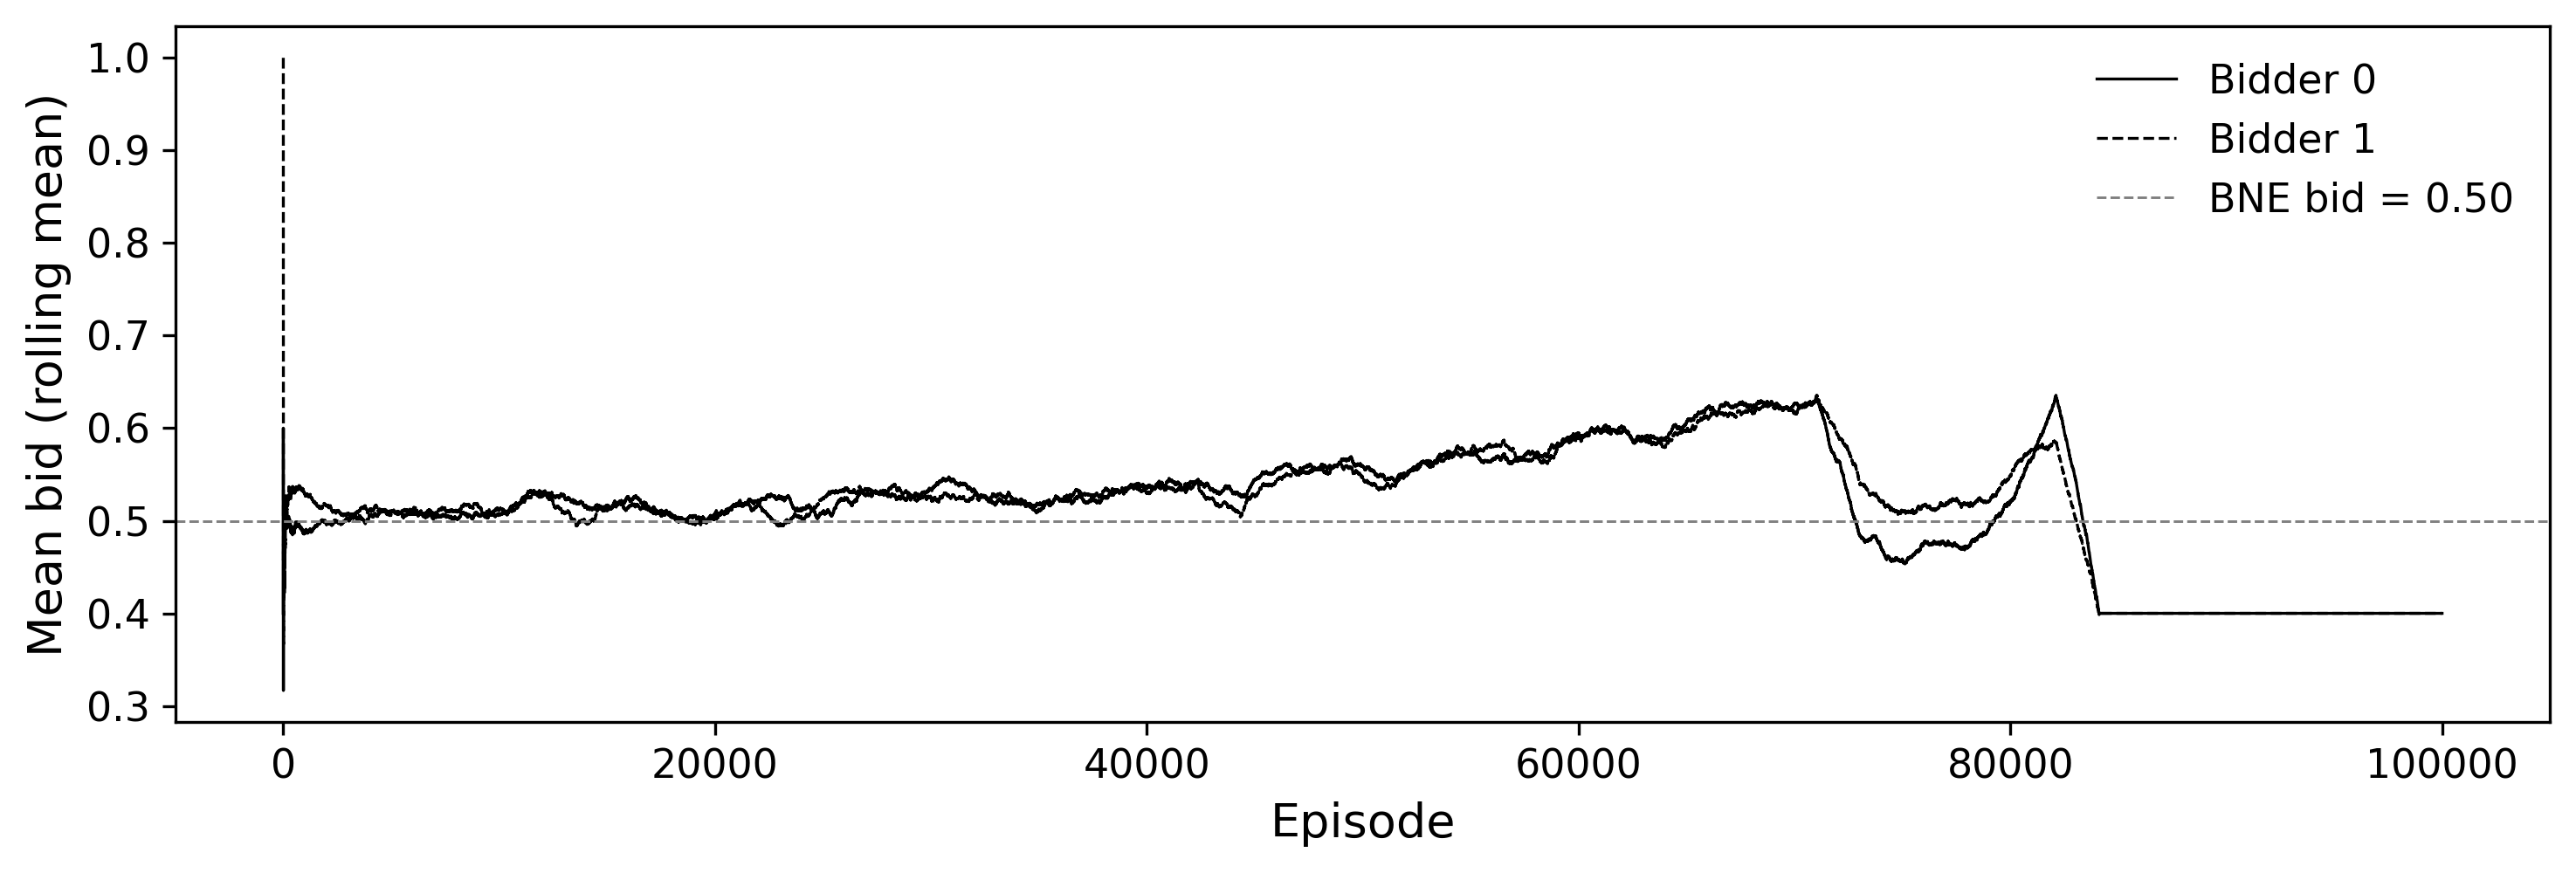
\includegraphics[width=0.75\textwidth]{e1a_trace}
\caption{Representative learning trajectory for a single Experiment~1a trial with a first-price auction, two bidders, and Boltzmann exploration. Per-bidder mean bids (rolling 200-episode mean) converge towards competitive levels over the 10{,}000 episodes shown.}
\label{fig:e1a_trace}
\end{figure}

\subsection{Factorial Analysis of Revenue}

The number of bidders is the dominant factor for end-state revenue, with $|t| = \ExpOneARevFactorTOne$. The shift from two to four bidders raises revenue by \ExpOneARevTopPctEffect{} percent of the grand mean, which is roughly \ExpOneARevTopVsAuctionRatio{} times larger than the effect of auction format. The discount factor $\gamma$ ranks second ($|t| = \ExpOneARevFactorTTwo$) and update mode third ($|t| = \ExpOneARevFactorTThree$). \Cref{tab:exp1a_ranked_rev} lists all significant effects ordered by absolute $t$-statistic.

\begin{table}[H]
\centering
\caption{Experiment 1a: Significant effects for average revenue ($p < 0.05$), ranked by $|t|$.}
\label{tab:exp1a_ranked_rev}
\begin{tabular}{lrrl}
\toprule
\textbf{Effect} & \textbf{Coeff.} & \textbf{$|t|$} & \textbf{Direction} \\
\midrule
Number of bidders & 0.0871 & 17.75 & + \\
Discount factor ($\gamma$) & -0.0453 & 9.23 & $-$ \\
Update mode & 0.0366 & 7.45 & + \\
Discount factor ($\gamma$) $\times$ Number of bidders & 0.0298 & 6.09 & + \\
Auction format $\times$ Number of bidders & -0.0276 & 5.63 & $-$ \\
Reserve price & 0.0250 & 5.10 & + \\
Reserve price $\times$ Information feedback & -0.0219 & 4.47 & $-$ \\
Auction format $\times$ Discount factor ($\gamma$) & -0.0215 & 4.38 & $-$ \\
Auction format $\times$ Update mode & -0.0193 & 3.94 & $-$ \\
Information feedback & 0.0182 & 3.71 & + \\
\bottomrule
\end{tabular}
\end{table}


Auction format has no significant main effect on end-state revenue ($|t| = \ExpOneARevAuctionT$, $p \ExpOneARevAuctionPFmt$). Mean revenue under first-price (\ExpOneARevMeanFPA) is within one percentage point of mean revenue under second-price (\ExpOneARevMeanSPA). This null result is consistent with revenue equivalence and provides the baseline against which the later experiments depart.

Format is not entirely inert. It interacts significantly with the number of bidders ($|t| = \ExpOneARevAuctionxNbidAbsT$) and with the discount factor ($|t| = \ExpOneARevAuctionxGammaAbsT$), meaning that the direction of the format effect depends on competitive thickness and on how patient the bidders are. The format gap is wider in thin markets than in thick markets, and wider when agents discount future payoffs less heavily. \Cref{fig:e1a_int_rev} visualises these two interactions.

\begin{figure}[H]
\centering
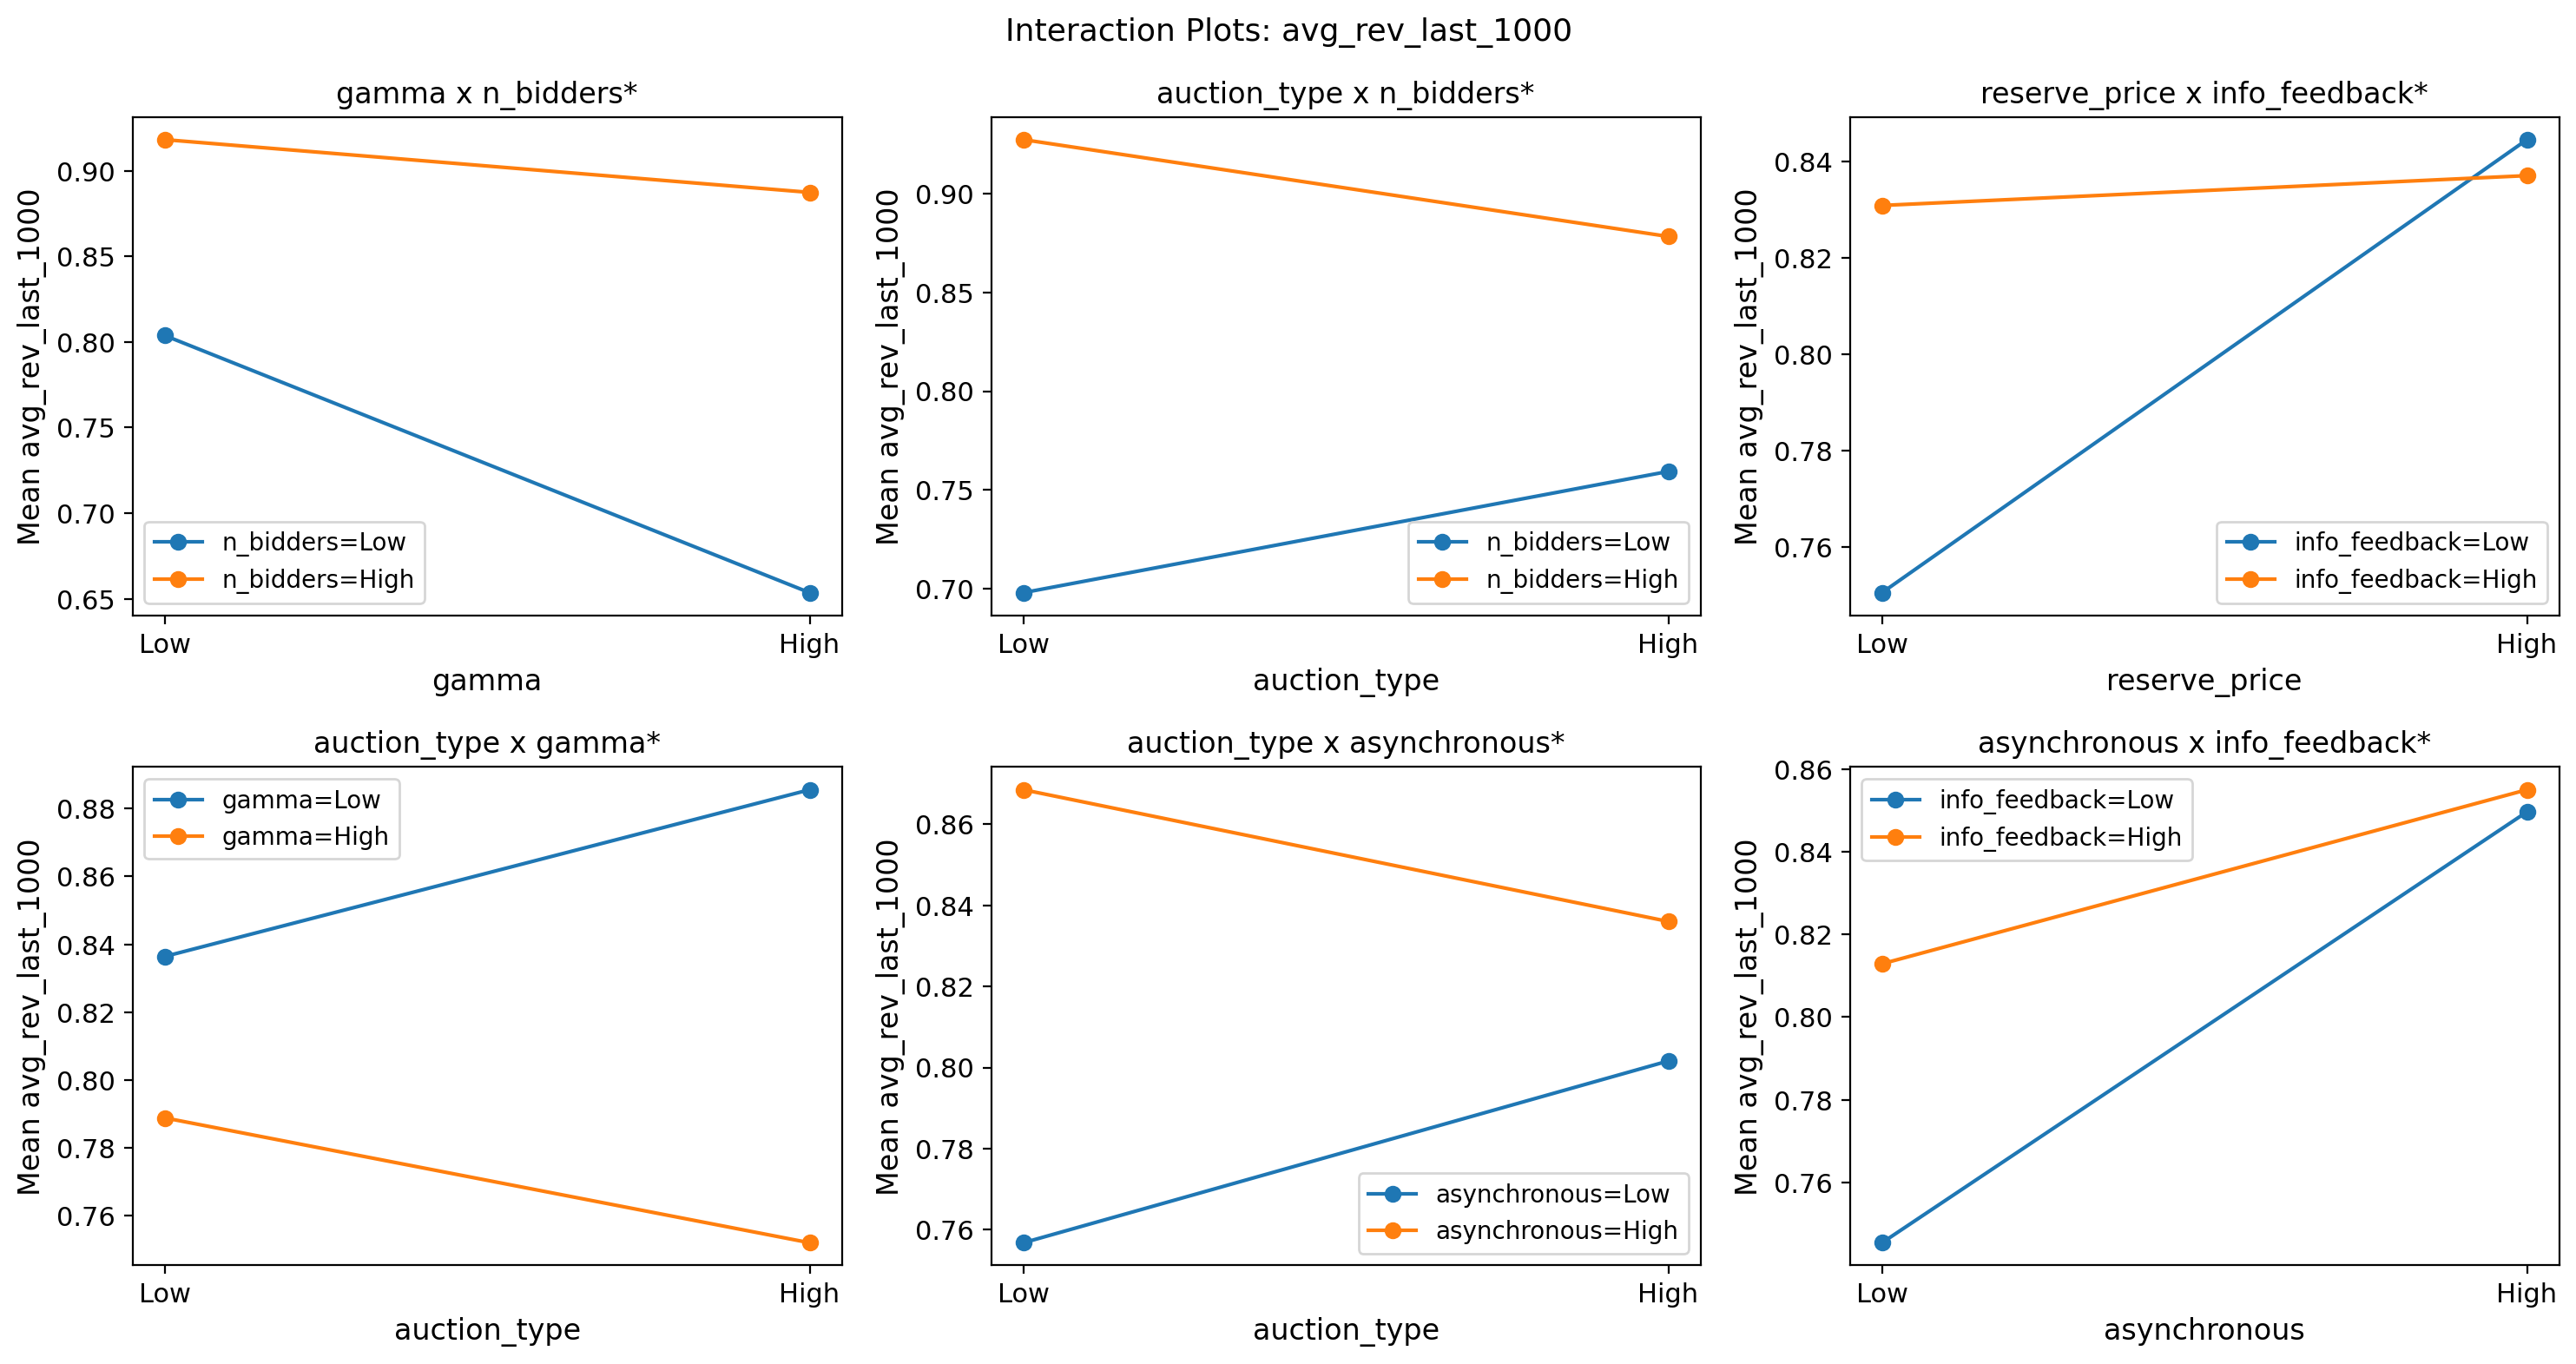
\includegraphics[width=0.75\textwidth]{e1a_int_rev}
\caption{Experiment~1a two-way interactions for end-state revenue. Non-parallel lines indicate that the effect of one factor depends on the level of the other.}
\label{fig:e1a_int_rev}
\end{figure}

\subsection{Summary of Experiment~1a}

Under constant valuations, the headline finding is that competitive thickness dominates every algorithmic design choice. Auction format has a negligible main effect but interacts with the number of bidders and the discount factor, so the choice of format matters in thin markets and under patient learning. Robustness checks reported in Appendix~\ref{ch:robustness} confirm that this ranking of factor effects survives multiple-testing correction, nonparametric model comparison, and quantile regression.

\section{Affiliated Valuations}
\label{sec:exp1b_results}

Experiment~1b keeps Q-learning but replaces constant valuations with the affiliated-signal model of \Cref{sec:env}. Each bidder draws a private signal $s_i$ uniformly from the eleven-point grid, and her valuation depends on her own signal and on the average of other bidders' signals via the affiliation parameter $\eta \in \{0, 0.5, 1\}$. The design is a $3 \times 2^3$ mixed-level factorial with 24 cells and 8 replicates, yielding 192 observations. Q-learning hyperparameters are fixed at the best-performing levels identified in Experiment~1a, specifically $\alpha = 0.10$, $\gamma = 0.95$, asynchronous updates, and $\varepsilon$-greedy exploration. \Cref{fig:e1b_trace} shows a representative trajectory.

\begin{figure}[H]
\centering
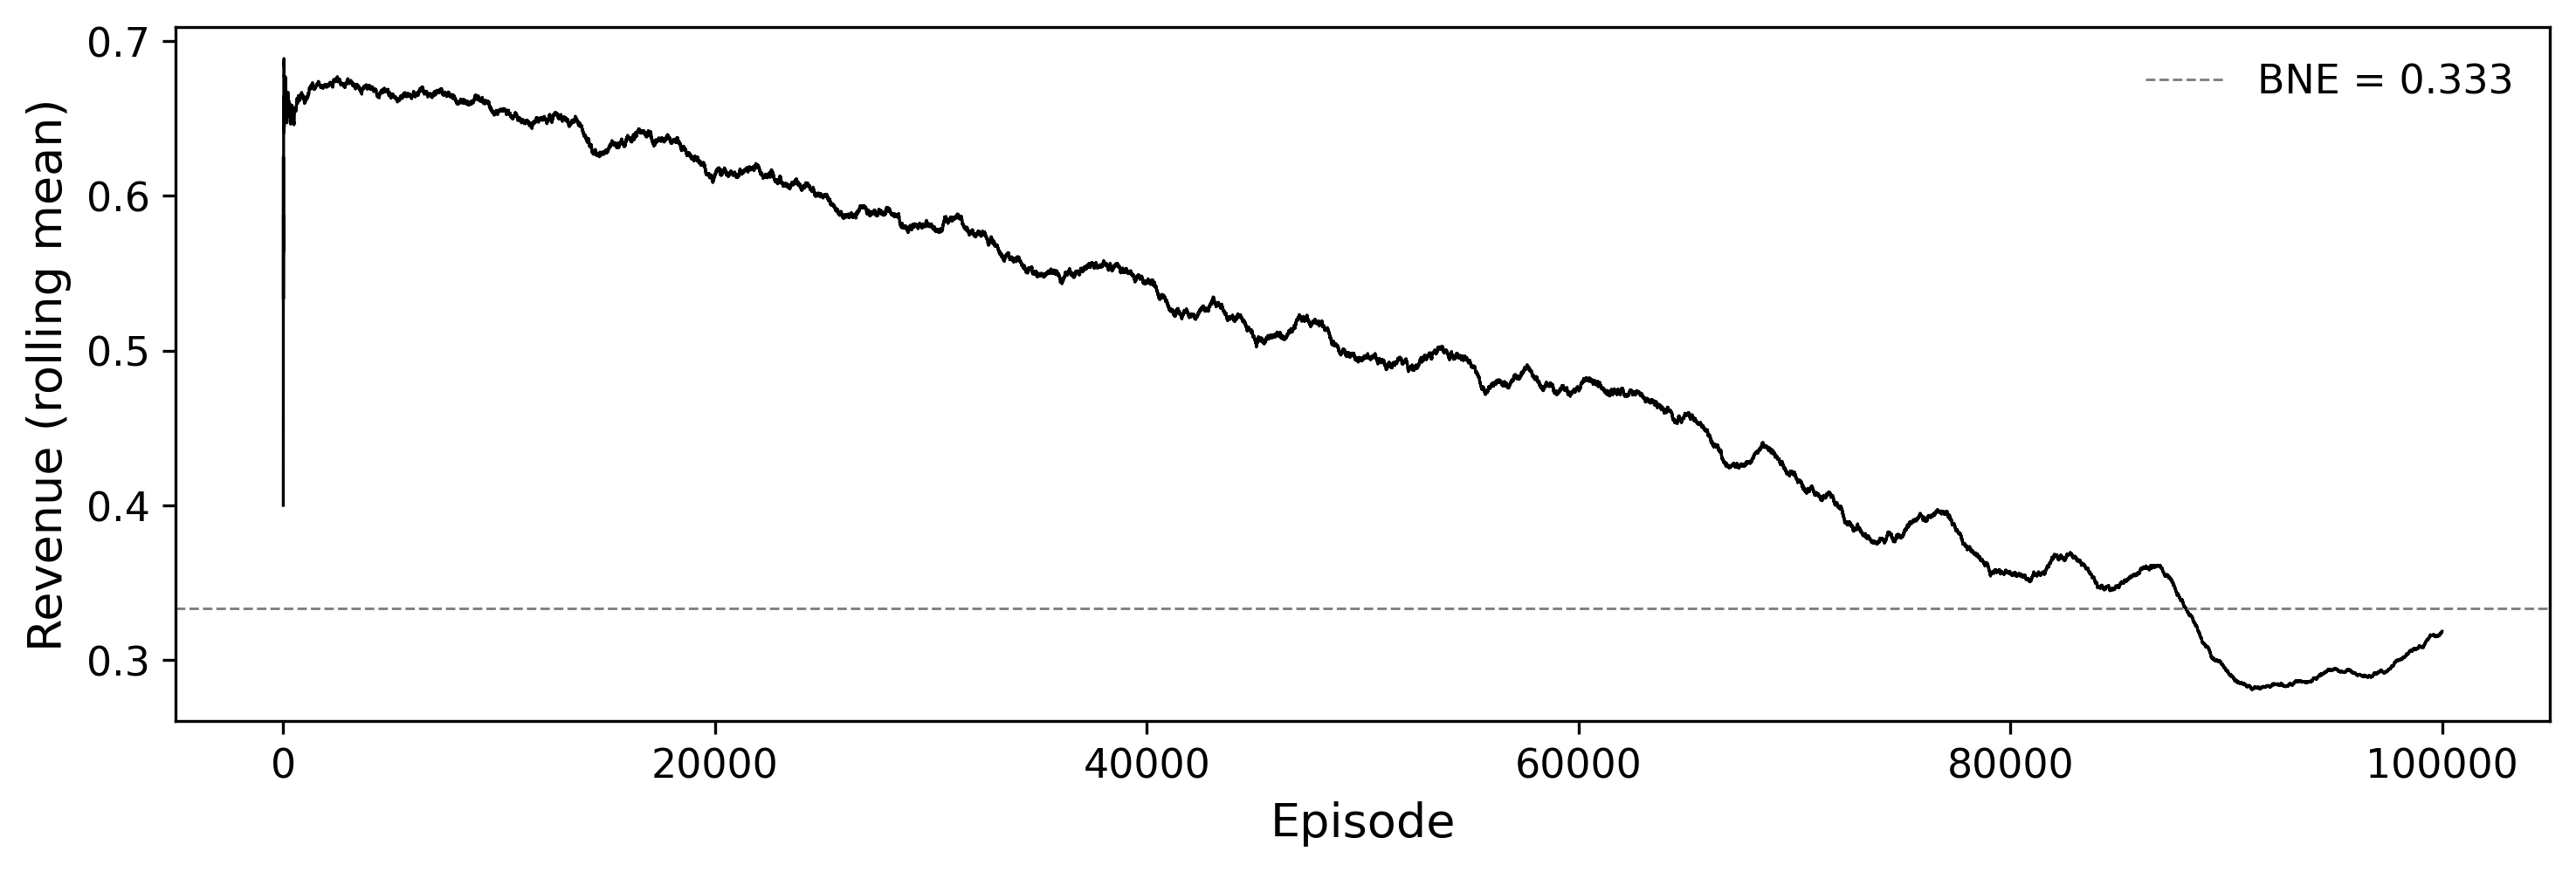
\includegraphics[width=0.75\textwidth]{e1b_trace}
\caption{Representative learning trajectory for a single Experiment~1b trial with a first-price auction, two bidders, and affiliation $\eta = 0.5$. Rolling-mean revenue stabilises within 10{,}000 episodes.}
\label{fig:e1b_trace}
\end{figure}

\subsection{Factorial Analysis of Revenue}

The number of bidders remains the dominant factor ($|t| = \ExpOneBRevNbidAbsT$), with the low-to-high shift raising revenue by \ExpOneBRevTopPctEffect{} percent of the grand mean. Auction format is now statistically significant but economically modest ($|t| = \ExpOneBRevAuctionT$, $p \ExpOneBRevAuctionPFmt$); first-price auctions generate lower end-state revenue, with mean \ExpOneBRevMeanFPA{} versus \ExpOneBRevMeanSPA{} under second-price. \Cref{tab:exp1b_ranked_rev} lists all significant effects.

\begin{table}[H]
\centering
\caption[Experiment 1b: significant effects for average revenue ($p < 0.05$), ranked by $|t|$]{\textbf{Experiment 1b: significant effects for average revenue ($p < 0.05$), ranked by $|t|$.}}
\label{tab:exp1b_ranked_rev}
\begin{tabular}{lrrl}
\toprule
\textbf{Effect} & \textbf{Coeff.} & \textbf{$|t|$} & \textbf{Direction} \\
\midrule
Number of bidders & 0.0552 & 6.53 & + \\
State information & -0.0495 & 5.85 & $-$ \\
Auction format $\times$ Number of bidders & -0.0285 & 3.38 & $-$ \\
Auction format & -0.0268 & 3.17 & $-$ \\
Number of bidders $\times$ State information & -0.0263 & 3.11 & $-$ \\
\bottomrule
\end{tabular}
\end{table}


The affiliation parameter $\eta$ has no significant effect on any primary outcome, despite spanning the full range from independent private values to near-common values. Revenue equivalence holds under this signal model because signals are drawn independently, so theory predicts no affiliation effect at equilibrium; the Q-learning agents reproduce this prediction even though they do not compute equilibrium bids directly.

The number of bidders moderates the auction-format effect. \Cref{fig:e1b_int_rev} shows the interaction plot for revenue. The first-price revenue penalty is larger in thin markets and shrinks in thicker markets, so the format gap and the competitive-thickness effect partially offset when many bidders compete.

\begin{figure}[H]
\centering
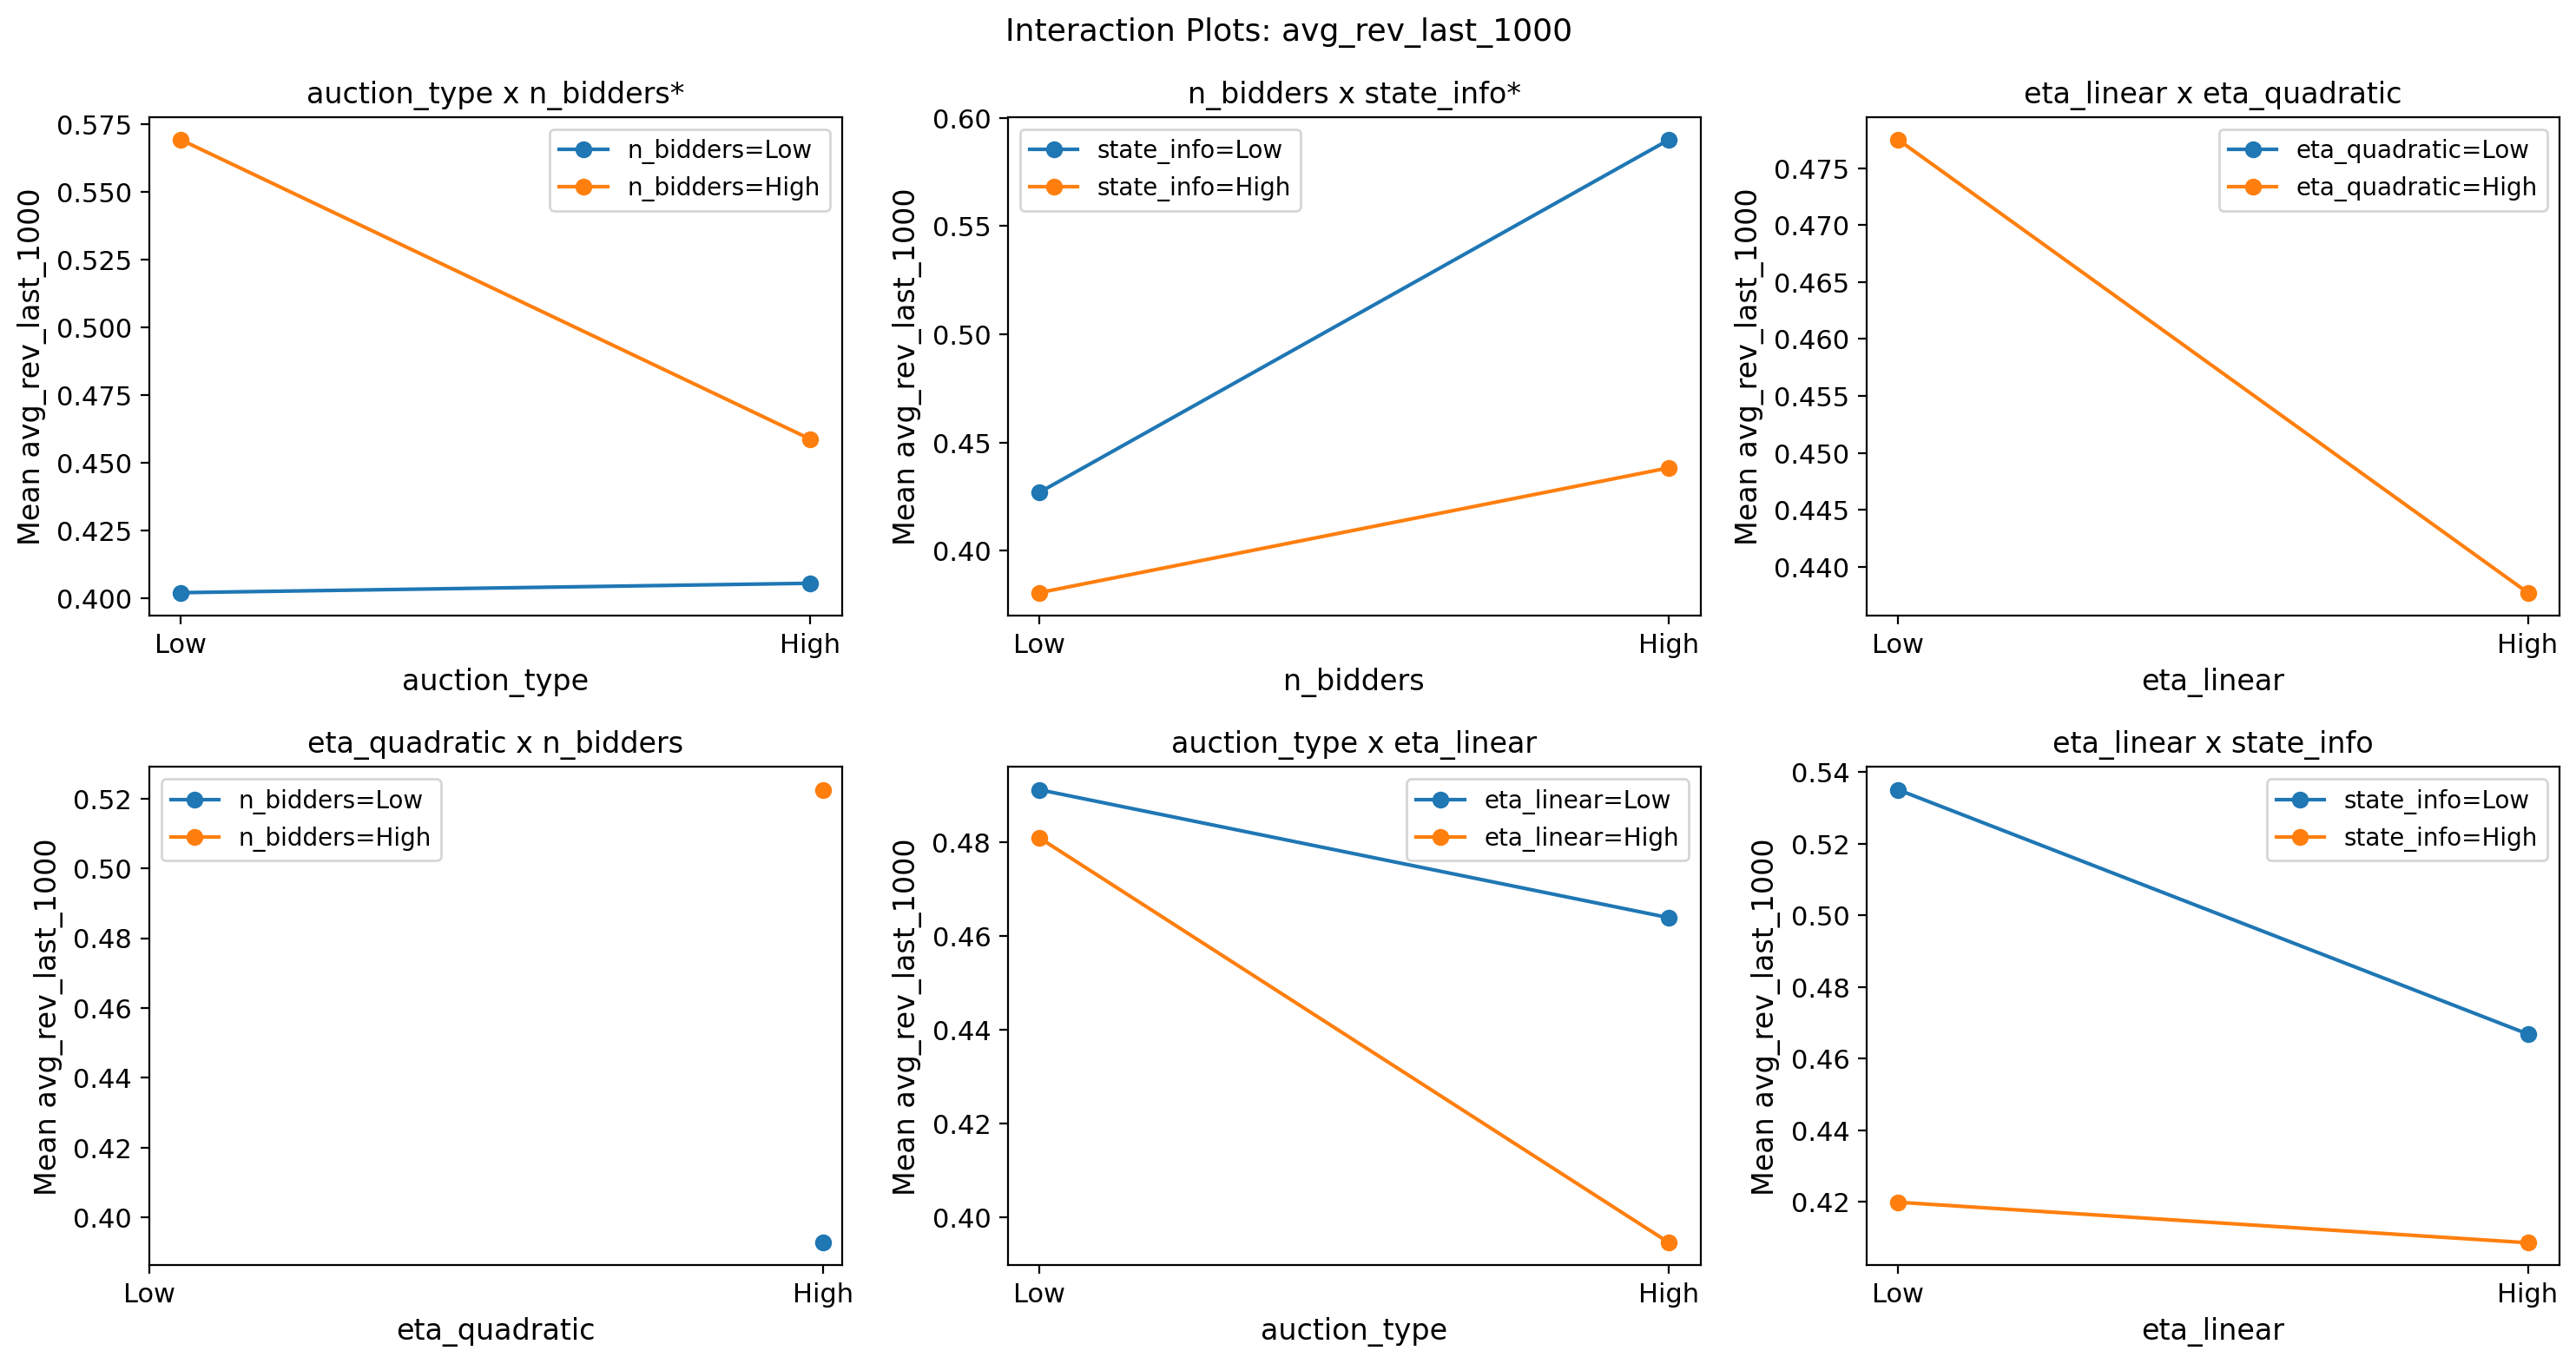
\includegraphics[width=0.75\textwidth]{e1b_int_rev}
\caption{Experiment~1b two-way interactions for end-state revenue. The auction-format-by-number-of-bidders and auction-format-by-state-information interactions are the strongest non-additive effects.}
\label{fig:e1b_int_rev}
\end{figure}

\subsection{Learning Phase versus Steady State}

End-state and lifetime revenue reveal different patterns. Both formats generate higher revenue during the learning phase than after convergence, but first-price auctions earn a learning-phase premium roughly three times larger than second-price.\footnote{Measured as the difference between mean lifetime revenue and mean end-state revenue. First-price: \ExpOneBAllMeanFPA{} lifetime versus \ExpOneBEndMeanFPA{} end-state, for a premium of \ExpOneBFPAPremium. Second-price: \ExpOneBAllMeanSPA{} versus \ExpOneBEndMeanSPA, for a premium of \ExpOneBSPAPremium.} When revenue is averaged over the full trajectory rather than the final 1{,}000 episodes, the auction-format main effect loses significance ($|t| = \ExpOneBAllRevAuctionAbsT$, $p \ExpOneBAllRevAuctionPFmt$), so the two formats become statistically indistinguishable on lifetime revenue. The auction-format-by-number-of-bidders interaction survives both measures and in fact reverses sign. With two bidders, first-price auctions yield higher lifetime revenue, while with four bidders, second-price auctions yield higher lifetime revenue.

\subsection{Summary of Experiment~1b}

Under affiliated valuations, the ranking of factors is stable. The number of bidders remains dominant, first-price auctions generate modestly lower end-state revenue than second-price, and affiliation itself has no measurable effect on any outcome. The lifetime-versus-end-state comparison shows that first-price auctions pass through a period of higher revenue during learning before settling at a lower steady state, which partially offsets the convergence gap. As in Experiment~1a, robustness checks in Appendix~\ref{ch:robustness} confirm these rankings.

\section{What Q-Learning Establishes}
\label{sec:qlearning_summary}

Across both sub-experiments, the number of bidders is the strongest determinant of seller outcomes, the discount factor is second most important where varied, and auction format is either inert (Experiment~1a) or modest (Experiment~1b). Affiliation does not matter at all under Q-learning, which stands in tension with the \citet{MilgromWeber1982} prediction that affiliated signals should favour second-price auctions. I do not speculate about which feature of Q-learning blunts the affiliation effect; the finding is simply that the algorithms I study do not track this aspect of the signal structure. Experiments~2a and~2b in the next chapter test whether more sophisticated contextual-bandit learners recover the classical pattern.

\chapter{Contextual Bandit Experiments}
\label{ch:bandits}

This chapter reports the two contextual-bandit sub-experiments. Experiment~2a replaces Q-learning with LinUCB (linear upper confidence bound) under the affiliated-signal model of Experiment~1b, and Experiment~2b replaces LinUCB with Thompson Sampling. The motivation is that contextual bandits can in principle use the signal context to refine their bids, which raises the question of whether more sophisticated learners recover the classical affiliation-based revenue ranking that Q-learning failed to produce. Both algorithms are defined in Chapter~\ref{ch:auctions_and_algorithms}; the present chapter focuses on the factorial analysis of their outputs.

\section{LinUCB}
\label{sec:exp2a_results}

Experiment~2a uses a mixed-level factorial that crosses seven binary factors with the three-level affiliation parameter (the $3 \times 2^7$ structure from Chapter~\ref{ch:design_and_inference}). The factors are auction format, number of bidders, reserve price, bandit exploration intensity, context richness, regularisation $\lambda$, memory decay $\delta$, and affiliation $\eta$. The design has 384 cells, replicated twice for \ExpTwoANobs{} observations. \Cref{tab:exp2_params_summary} summarises the factors.

\begin{table}[H]
\centering
\caption{Experiment~2a and 2b factor levels. Memory decay and regularisation are used only in Experiment~2a because preliminary screening found them negligible for Thompson Sampling.}
\label{tab:exp2_params_summary}
\begin{tabular}{l l l}
\toprule
\textbf{Factor} & \textbf{Low} ($-1$) & \textbf{High} ($+1$)\\
\midrule
Auction format & Second-price & First-price \\
Number of bidders $n$ & 2 & 4 \\
Reserve price $r$ & 0.0 & 0.3 \\
Exploration intensity & Low & High \\
Context richness & Signal only & Signal plus winner \\
Regularisation $\lambda$ (2a only) & 0.1 & 5.0 \\
Memory decay $\delta$ (2a only) & 1.0 & 0.999 \\
Affiliation $\eta$ & \multicolumn{2}{l}{three levels: 0, 0.5, 1} \\
\bottomrule
\end{tabular}
\end{table}

Each run lasts 100{,}000 rounds. \Cref{fig:e2a_trace} shows a representative bid function late in training, plotted against the theoretical bid function.

\begin{figure}[H]
\centering
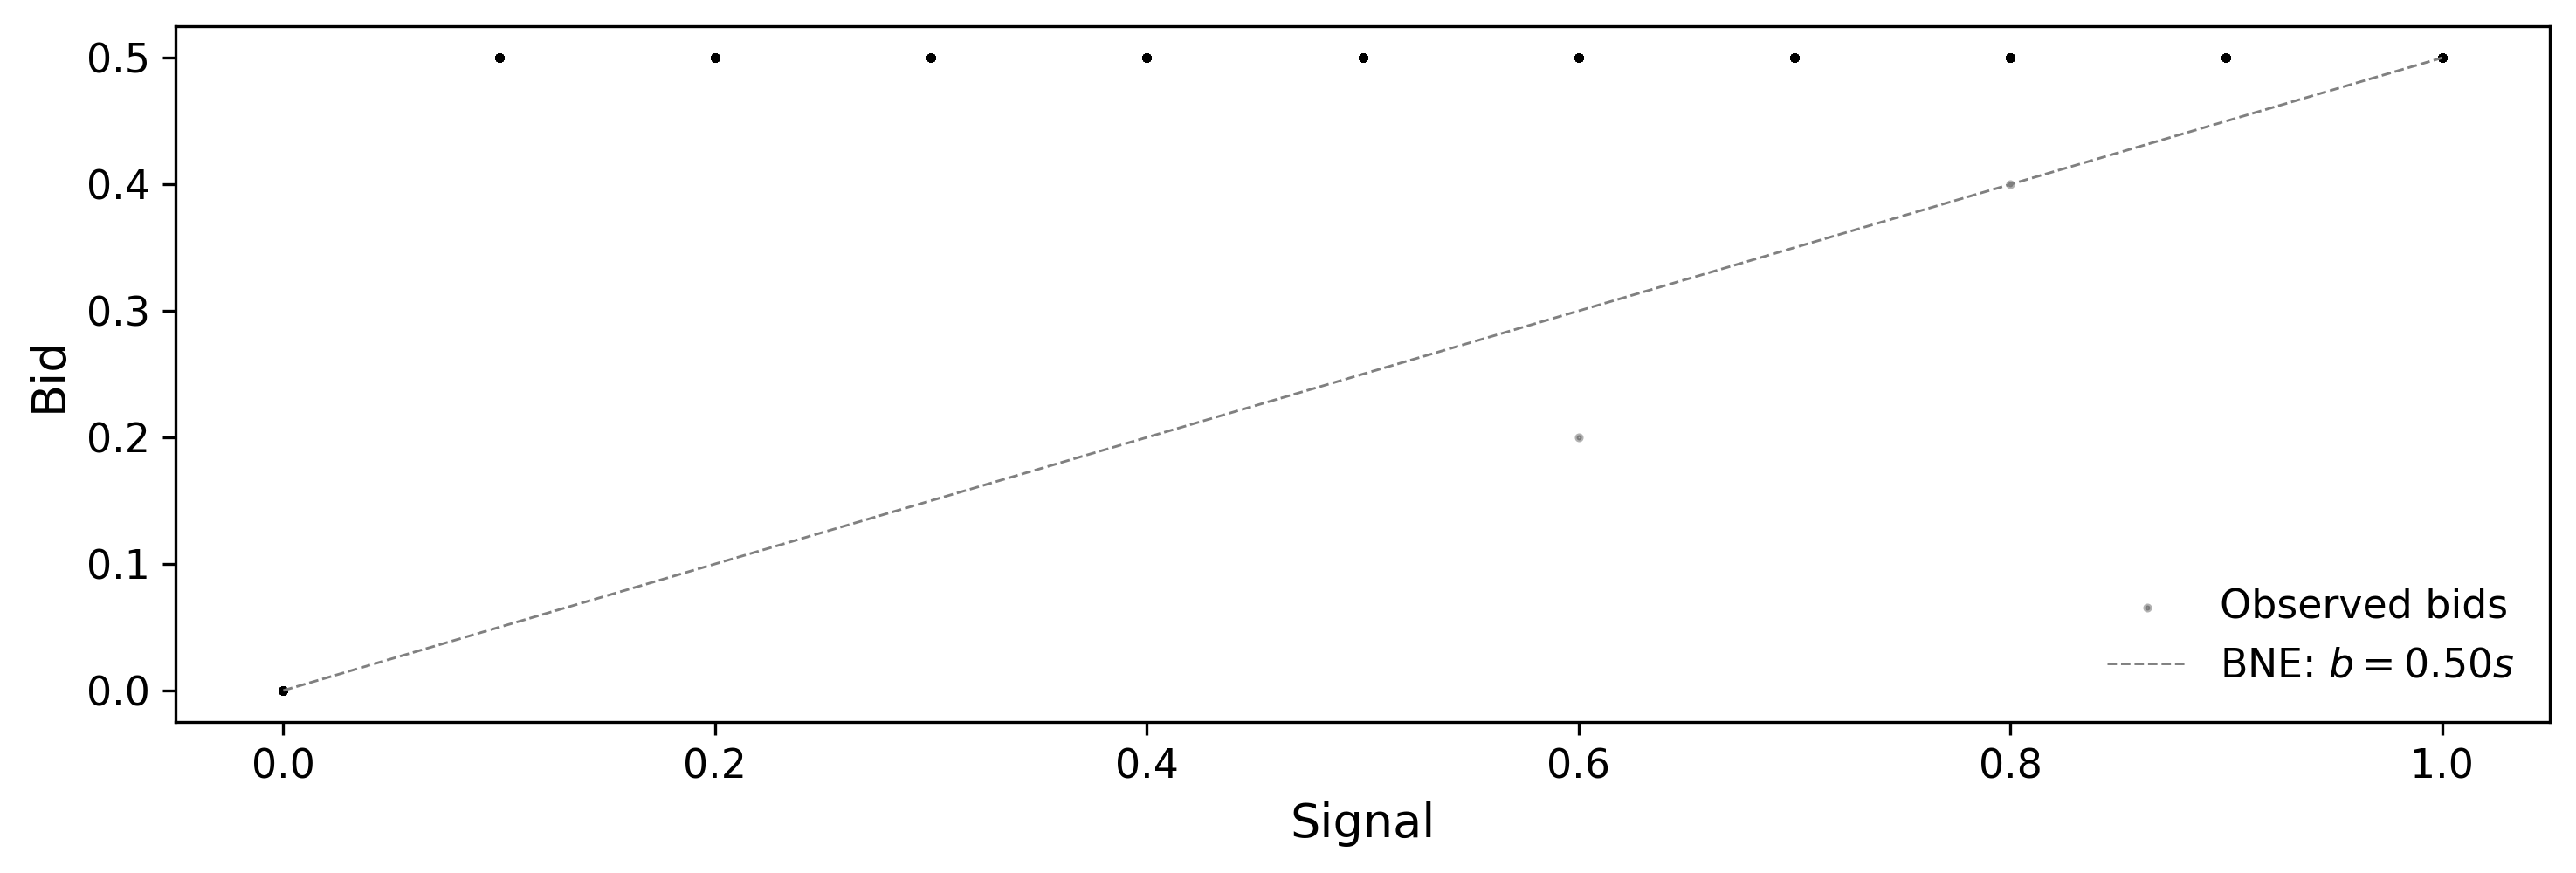
\includegraphics[width=0.75\textwidth]{e2a_trace}
\caption{Representative LinUCB bid function from a single Experiment~2a trial with a first-price auction, two bidders, and affiliation $\eta = 0.5$. Points show bids versus signals in the final 1{,}000 rounds; the reference line shows the symmetric Bayes-Nash bid function.}
\label{fig:e2a_trace}
\end{figure}

\subsection{Factorial Analysis of Revenue}

The number of bidders dominates ($|t| = \ExpTwoARevFactorTOne$), producing its largest effect of any experiment in the thesis. The shift from two to four bidders raises revenue by \ExpTwoARevTopPctEffect{} percent of the grand mean, roughly \ExpTwoARevTopVsAuctionRatio{} times the effect of auction format. \Cref{tab:exp2a_ranked_rev} ranks all significant effects.

\begin{table}[H]
\centering
\caption{Experiment 2a: Significant effects for average revenue ($p < 0.05$), ranked by $|t|$.}
\label{tab:exp2a_ranked_rev}
\begin{tabular}{lrrl}
\toprule
\textbf{Effect} & \textbf{Coeff.} & \textbf{$|t|$} & \textbf{Direction} \\
\midrule
Number of bidders & 0.1308 & 33.90 & + \\
Auction format & -0.0482 & 12.49 & $-$ \\
Number of bidders $\times$ Reserve price & -0.0400 & 10.36 & $-$ \\
Auction format $\times$ Number of bidders & -0.0245 & 6.35 & $-$ \\
Reserve price $\times$ Context richness & -0.0223 & 5.78 & $-$ \\
Affiliation (linear) & -0.0135 & 5.71 & $-$ \\
Affiliation (linear) $\times$ Affiliation (quadratic) & -0.0135 & 5.71 & $-$ \\
Exploration intensity & -0.0168 & 4.37 & $-$ \\
Auction format $\times$ Reserve price & 0.0150 & 3.88 & + \\
Exploration intensity $\times$ Context richness & 0.0137 & 3.54 & + \\
\bottomrule
\end{tabular}
\end{table}


Auction format is significant and negative ($|t| = \ExpTwoARevAuctionT$, $p \ExpTwoARevAuctionPFmt$), meaning first-price auctions reduce revenue. Mean revenue under first-price is \ExpTwoARevMeanFPA{} versus \ExpTwoARevMeanSPA{} under second-price, a gap of roughly 19 percent in favour of second-price. The direction of this effect matches the revenue ranking that \citet{MilgromWeber1982} derive for affiliated signals. I do not claim that LinUCB is recovering the exact equilibrium bid function; I report only that LinUCB produces revenue outcomes that are directionally aligned with the classical affiliation result, a pattern absent under Q-learning.

Interactions carry much of the remaining structure. \Cref{fig:e2a_int_rev} shows the strongest two-way interactions. Exploration intensity moderates the auction-format effect, and the number of bidders moderates the exploration effect, so the joint effect of competitive pressure and algorithm configuration is larger than the sum of the two main effects.

\begin{figure}[H]
\centering
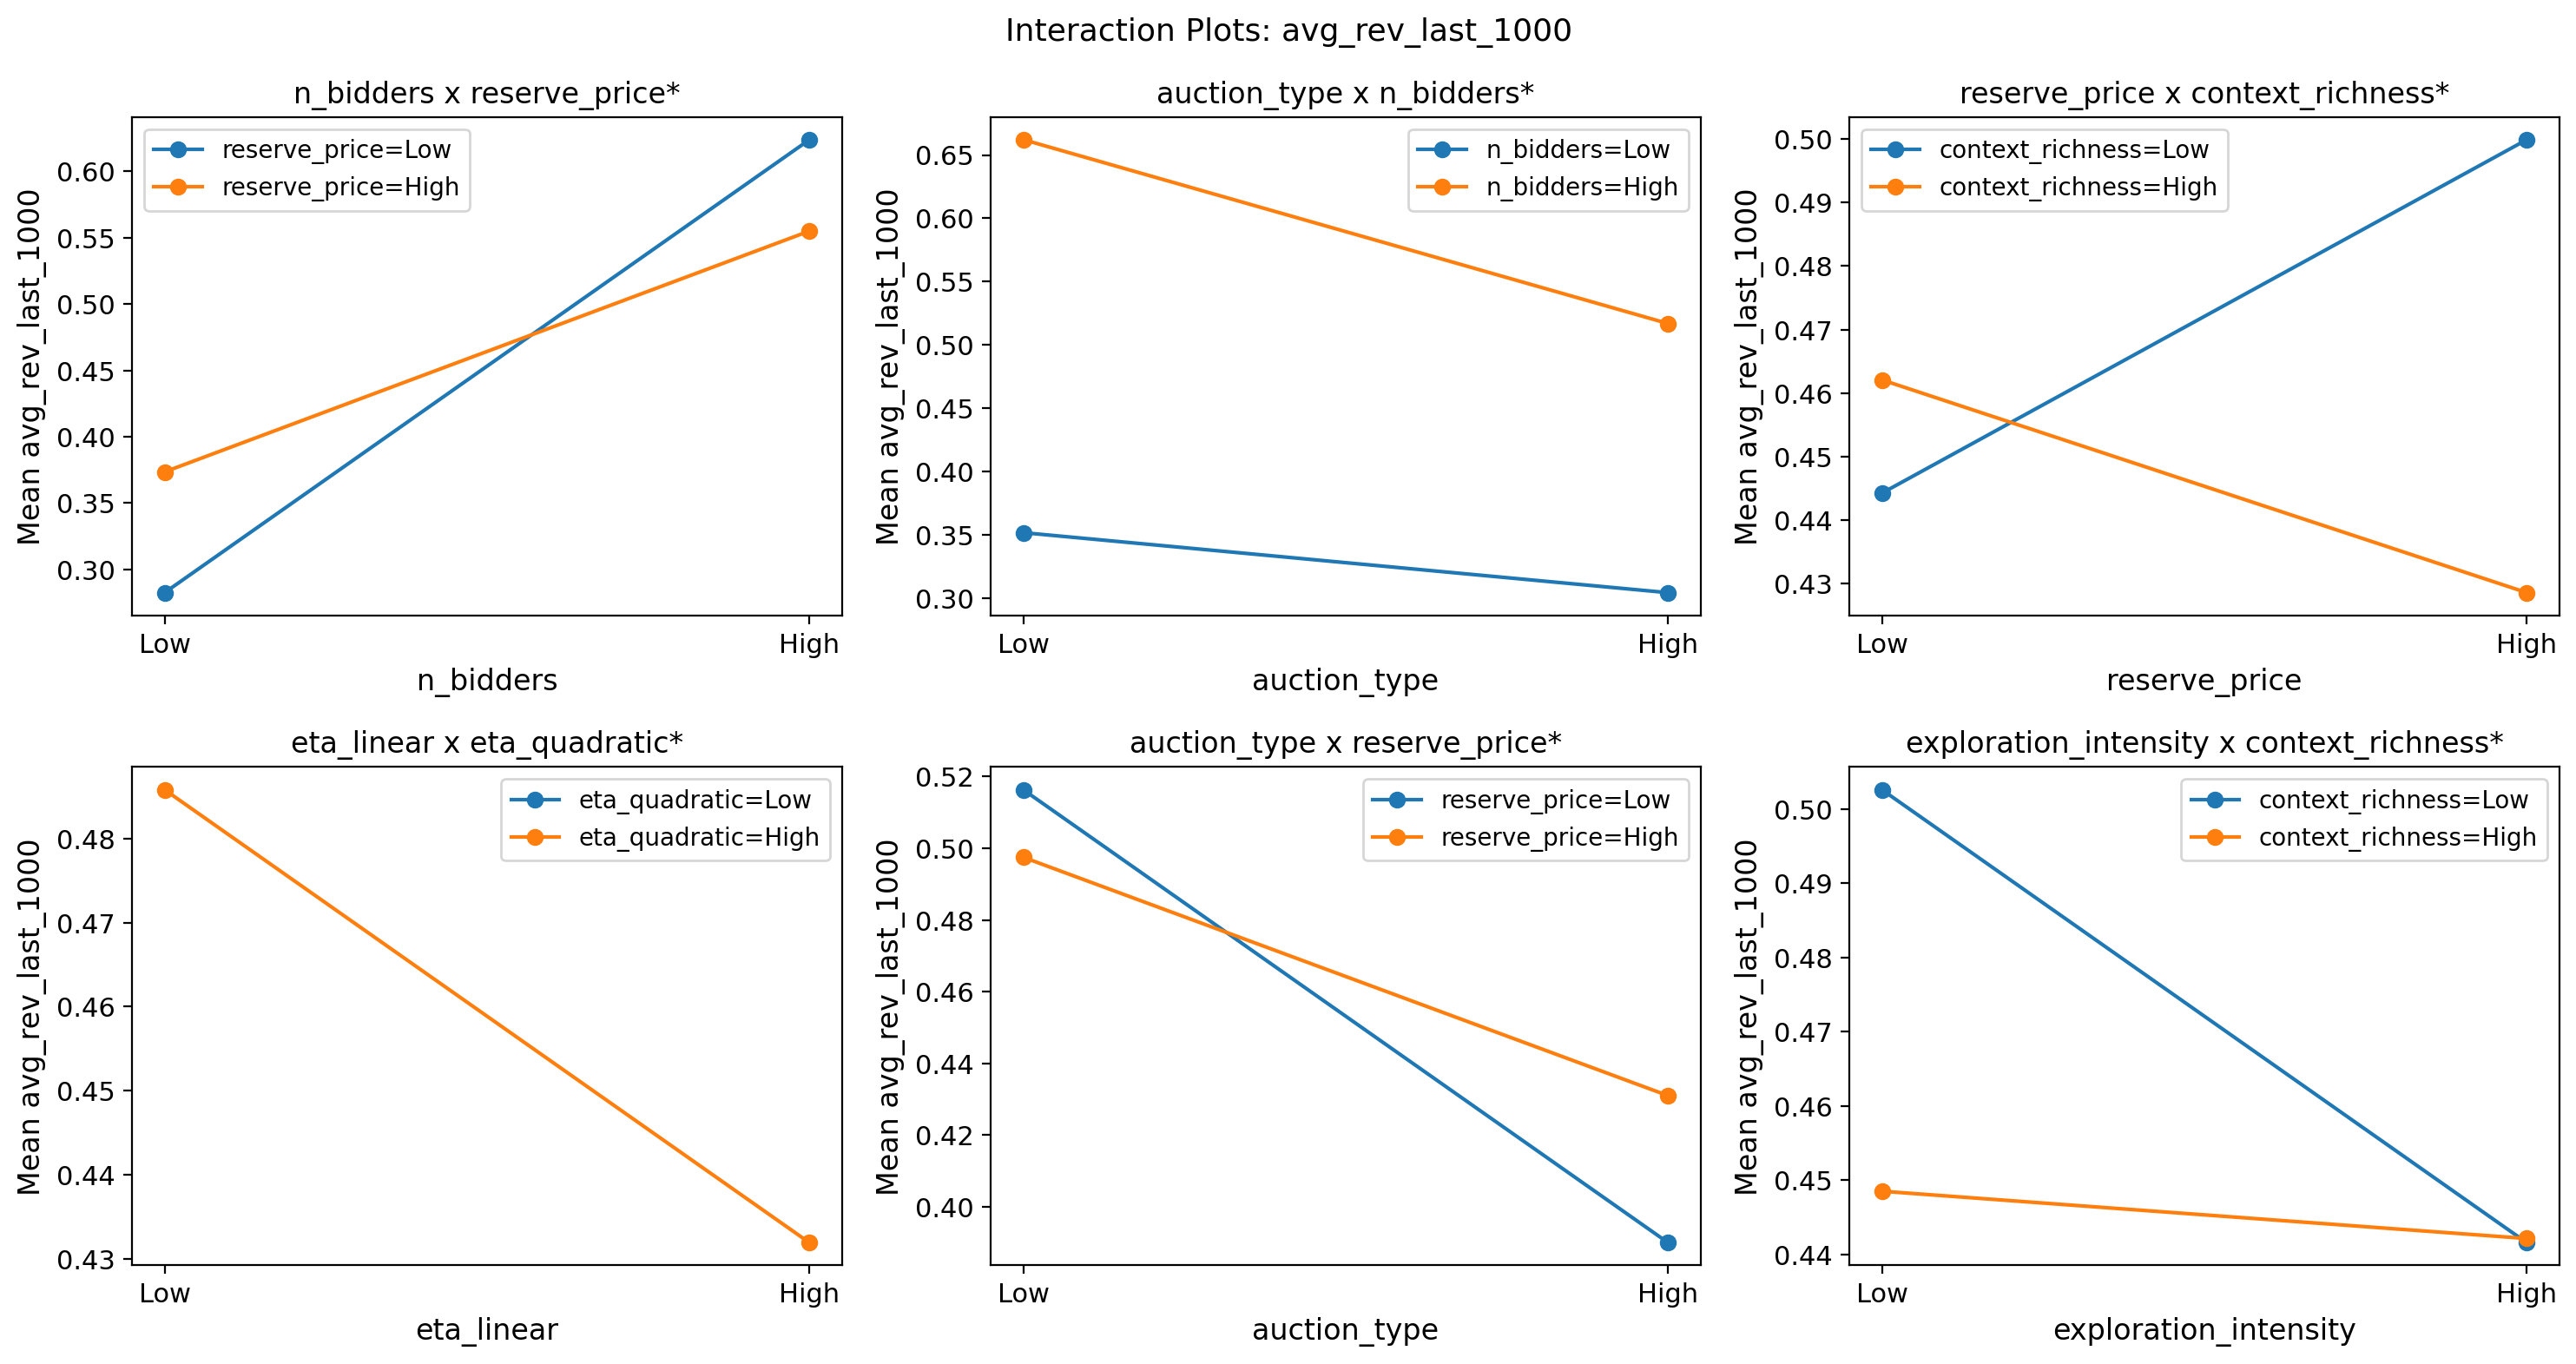
\includegraphics[width=0.75\textwidth]{e2a_int_rev}
\caption{Experiment~2a two-way interactions for end-state revenue under LinUCB.}
\label{fig:e2a_int_rev}
\end{figure}

Tuning parameters are essentially inert. Regularisation $\lambda$ and memory decay $\delta$ both fail to produce significant main effects on revenue, even though they shape the LinUCB update rule directly. This is consistent with the Sobol decomposition reported in \Cref{sec:bandits_summary}, where algorithmic parameters collectively explain less than four percent of revenue variance.

\section{Thompson Sampling}
\label{sec:exp2b_results}

Experiment~2b replaces LinUCB with contextual Thompson Sampling under the same valuation model. Because Thompson Sampling explores through posterior sampling rather than an optimism bonus, regularisation and memory decay no longer enter as meaningful design levers, and the design shrinks to a mixed-level factorial with five binary factors and the three-level affiliation parameter (the $3 \times 2^5$ structure), for 96 cells replicated twice and \ExpTwoBNobs{} total observations. \Cref{fig:e2b_trace} shows a representative bid function.

\begin{figure}[H]
\centering
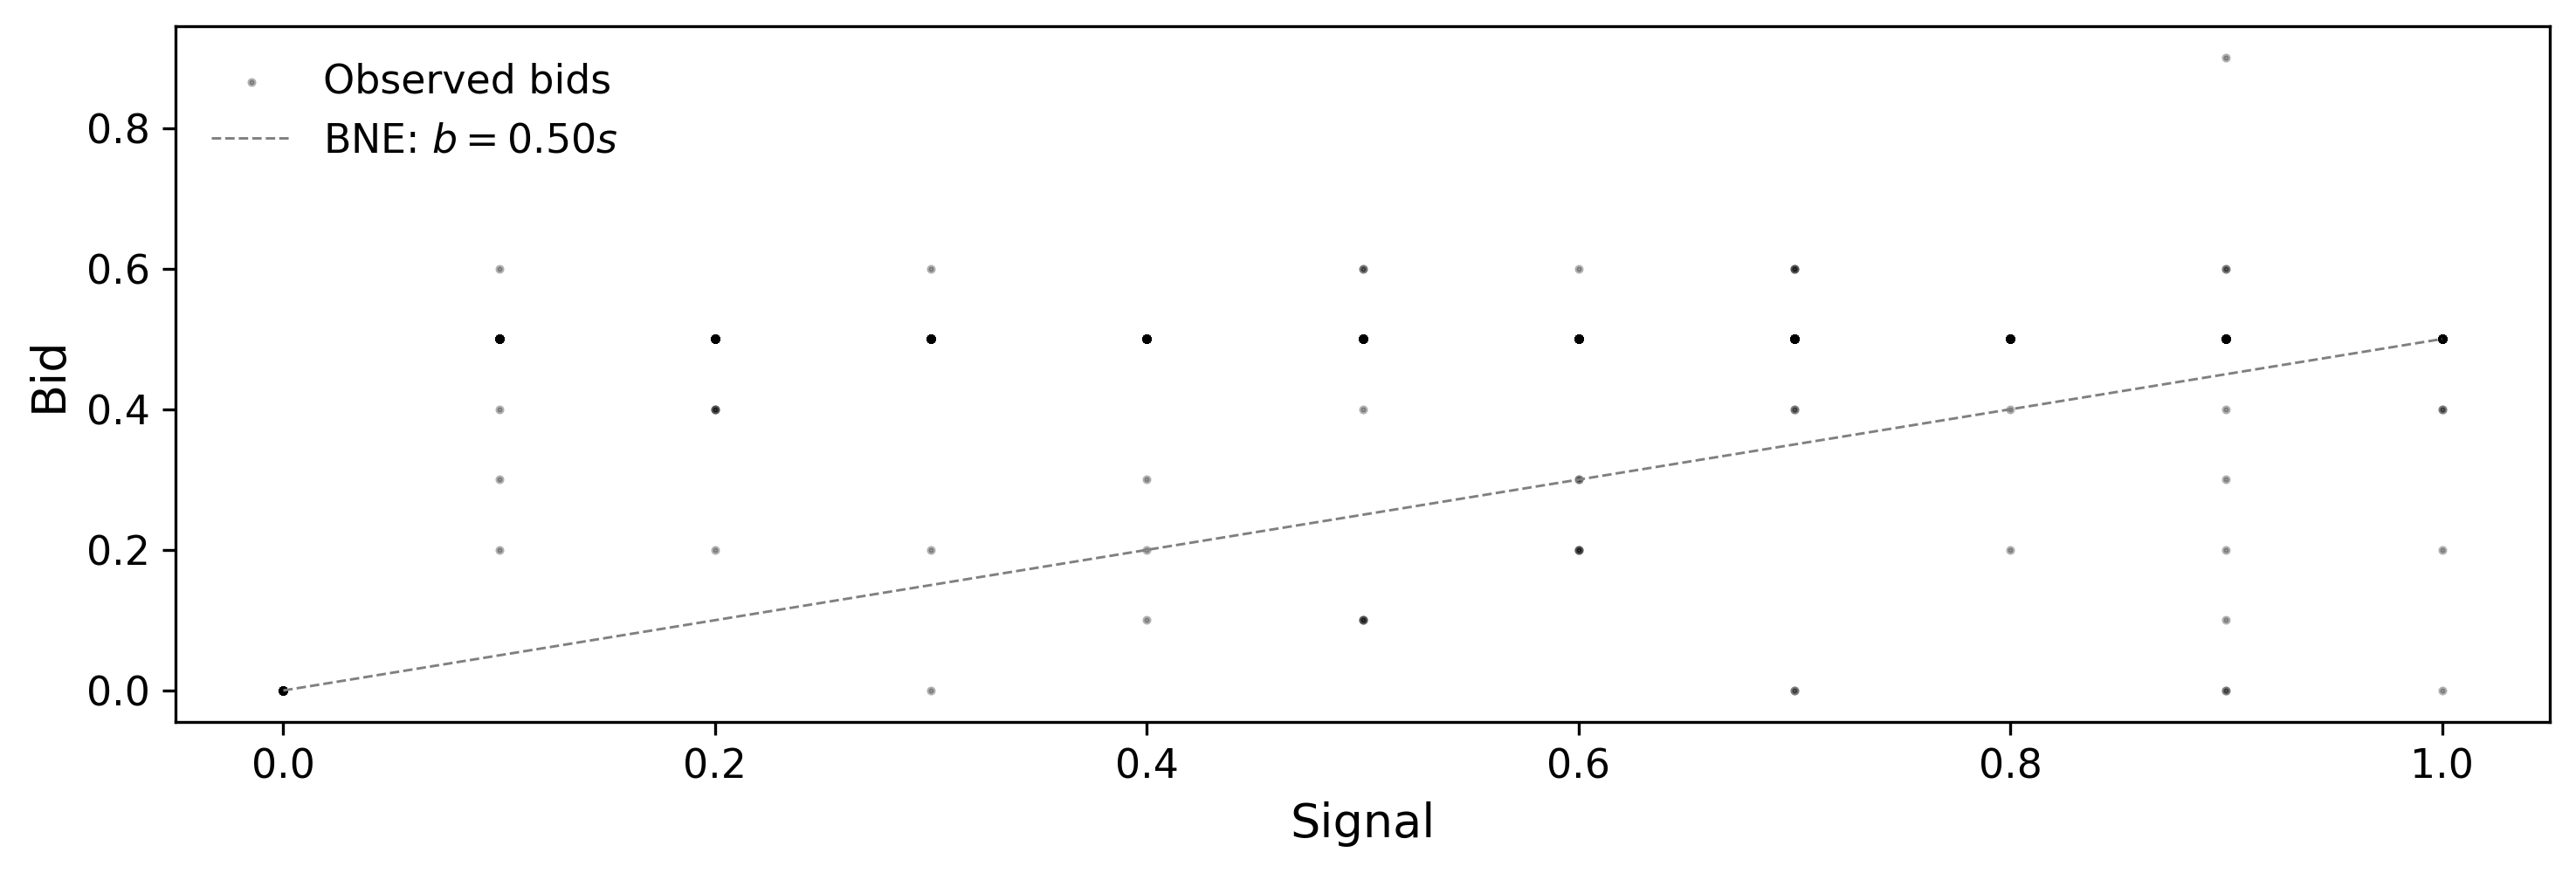
\includegraphics[width=0.75\textwidth]{e2b_trace}
\caption{Representative Thompson Sampling bid function from a single Experiment~2b trial with a first-price auction, two bidders, and affiliation $\eta = 0.5$.}
\label{fig:e2b_trace}
\end{figure}

\subsection{Factorial Analysis of Revenue}

The number of bidders is again the top factor ($|t| = \ExpTwoBRevFactorTOne$), followed by reserve price ($|t| = \ExpTwoBRevFactorTTwo$). \Cref{tab:exp2b_ranked_rev} lists all significant effects.

\begin{table}[H]
\centering
\caption[Experiment 2b: significant effects for average revenue ($p < 0.05$), ranked by $|t|$]{\textbf{Experiment 2b: significant effects for average revenue ($p < 0.05$), ranked by $|t|$.}}
\label{tab:exp2b_ranked_rev}
\begin{tabular}{lrrl}
\toprule
\textbf{Effect} & \textbf{Coeff.} & \textbf{$|t|$} & \textbf{Direction} \\
\midrule
Number of bidders & 0.0525 & 8.69 & + \\
Reserve price & -0.0480 & 7.95 & $-$ \\
Number of bidders $\times$ Context richness & 0.0284 & 4.71 & + \\
Auction format $\times$ Number of bidders & -0.0245 & 4.07 & $-$ \\
Auction format & -0.0231 & 3.83 & $-$ \\
Exploration intensity & -0.0204 & 3.38 & $-$ \\
Affiliation (linear) $\times$ Affiliation (quadratic) & -0.0117 & 3.18 & $-$ \\
Affiliation (linear) & -0.0117 & 3.18 & $-$ \\
Context richness & -0.0175 & 2.89 & $-$ \\
Number of bidders $\times$ Reserve price & -0.0174 & 2.88 & $-$ \\
\bottomrule
\end{tabular}
\end{table}


Auction format is significant and negative ($|t| = \ExpTwoBRevAuctionT$, $p \ExpTwoBRevAuctionPFmt$), with first-price yielding \ExpTwoBRevMeanFPA{} against \ExpTwoBRevMeanSPA{} for second-price. The format gap is smaller than under LinUCB, roughly \ExpTwoBRevGapPct{} percent versus \ExpTwoARevGapPct{} percent, but the direction is the same. \Cref{fig:e2b_int_rev} shows the strongest interactions.

\begin{figure}[H]
\centering
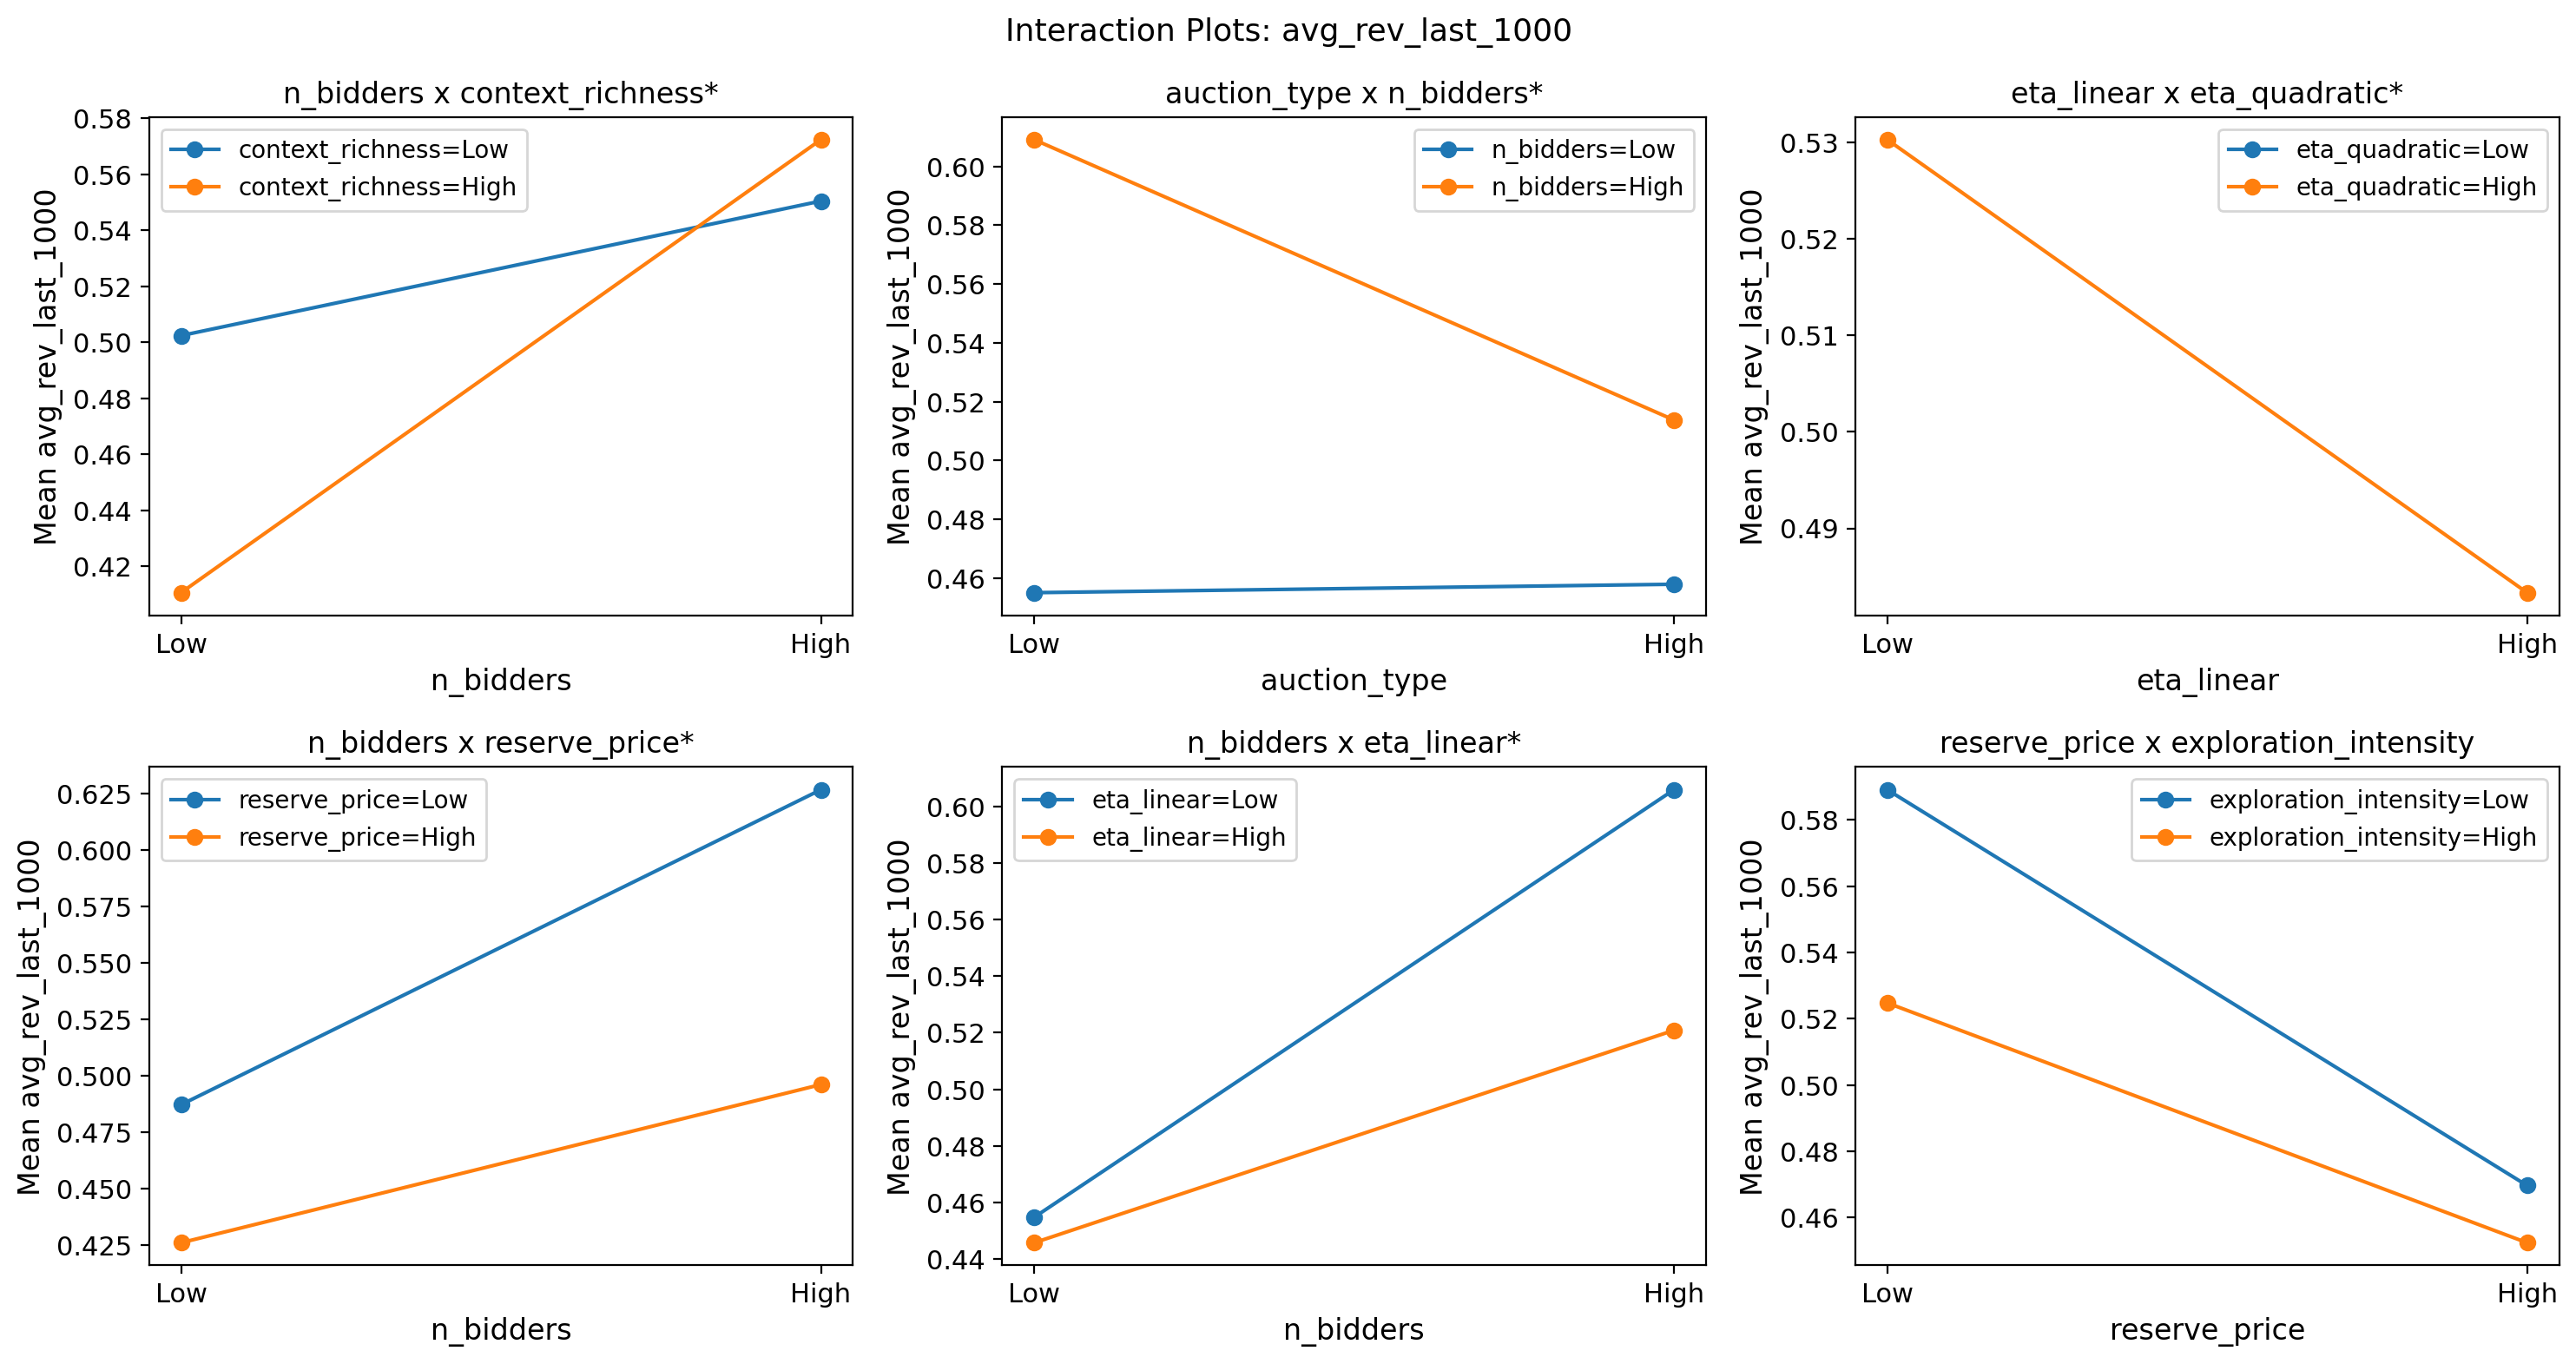
\includegraphics[width=0.75\textwidth]{e2b_int_rev}
\caption{Experiment~2b two-way interactions for end-state revenue under Thompson Sampling.}
\label{fig:e2b_int_rev}
\end{figure}

Unlike LinUCB, Thompson Sampling produces a more diffuse factor hierarchy. No single factor accounts for the lion's share of revenue variance, and several factors contribute in similar measure. This is consistent with the fact that posterior sampling injects randomness into exploration at every round, which tends to wash out the differences between factors that an optimism bonus would amplify. I emphasise that this is an observation about the input-output map, not a mechanistic claim.

\section{What Contextual Bandits Establish}
\label{sec:bandits_summary}

Two findings carry across both bandit sub-experiments. First, the number of bidders remains the dominant factor for revenue, and algorithmic hyperparameters are collectively inert. The Sobol variance decomposition reported in Appendix~\ref{ch:robustness} gives the number of bidders a total-order index of roughly 0.55 under LinUCB and 0.31 under Thompson Sampling, with algorithmic parameters all below 0.04. Second, and differently from Q-learning, auction format now has a clearly negative main effect on revenue. First-price auctions generate lower revenue under both bandit algorithms, which is directionally consistent with the \citet{MilgromWeber1982} revenue ranking for affiliated signals. The emergence of a non-trivial format effect under bandits, but not under tabular Q-learning, is the first piece of evidence that revenue consequences of auction design depend on the bidding technology.

Neither contextual-bandit algorithm improves seller welfare relative to Q-learning. Both generate slightly lower end-state revenue than Q-learning on average, and neither produces a competitive bid function that tracks the Bayes-Nash benchmark in absolute terms. The main shift from Q-learning to bandits is that the format-versus-affiliation comparison becomes informative rather than inert.

\chapter{Budget-Constrained Pacing Experiments}
\label{ch:pacing}

This chapter reports the two pacing sub-experiments. Experiment~3a studies bidders using multiplicative dual pacing in the spirit of \citet{Balseiro2019Learning}, and Experiment~3b replaces the dual update with a proportional-integral controller. Both experiments shift from unconstrained learning to budget-constrained bidding, the setting that dominates modern online advertising auctions. Two central questions structure the chapter. First, does the auction-format pattern observed under learning algorithms survive the move to pacing? Second, does the choice of pacing control law change the factor hierarchy?

\section{Shared Environment}
\label{sec:pacing_env}

Both experiments use the same auction environment. Each of $n \in \{2, 4\}$ advertisers participates in $D = 100$ episodes of $T = 1{,}000$ single-item auctions. Between episodes, budgets regenerate to their initial level while the control variables ($\mu$ for dual pacing, $\lambda$ for the PI controller) persist across episode boundaries, reflecting how daily ad-budget cycles work in practice. Valuations follow a log-normal model with bidder-specific asymmetry; each bidder draws a mean $\mu_i$ uniformly from $[0.5, 1.5]$ once per seed, and in each round the valuation is $v_{it} \sim \mathrm{LogNormal}(\mu_i, \sigma)$. Budgets per episode are $B_i = m \cdot \mathbb{E}[v_{it}] \cdot T$, where $m$ is the budget multiplier factor.

Both experiments use a full factorial in six binary factors (the $2^6$ design from Chapter~\ref{ch:design_and_inference}), which gives 64 cells replicated across eight random seeds for 512 observations. The factors common to both experiments are auction format, number of bidders $n$, budget multiplier $m$, reserve price $r$, and value dispersion $\sigma$. The sixth factor differs between the two experiments. Experiment~3a varies bidder objective (value-maximising versus utility-maximising), which determines whether the agent bids $v / \mu$ or $v / (1 + \mu)$. Experiment~3b varies controller aggressiveness, which scales the proportional and integral gains of the feedback rule by a factor of ten (from $a = 0.3$ to $a = 3.0$).

The factorial model explains a large share of revenue variance in both experiments, with $R^2 = \ExpThreeARevRsq$ for dual pacing and $R^2 = \ExpThreeBRevRsq$ for PI pacing. These $R^2$ values are a descriptive statement about model fit, not a claim that the estimated effects are identified in the econometric sense. The factorial design orthogonalises the inputs by construction, so the OLS coefficients unambiguously recover the partial-derivative effects of each input on the output of the simulator. What they do not recover is any causal parameter of an underlying economic model, since the simulator is the object of study and the black-box framing of the thesis treats it as such.

\section{Dual Pacing}
\label{sec:exp3a_results}

Experiment~3a uses multiplicative dual pacing. \Cref{fig:e3a_trace} shows a representative trajectory of the bid-to-value ratio across episodes. The bid-to-value ratio is the bid an agent submits divided by the valuation she draws in that round. A ratio below one means the agent shades her bid below her value. A ratio equal to one means she bids her full value, and a ratio above one means she overbids.

\begin{figure}[H]
\centering

\includegraphics[width=0.75\textwidth]{e3a_trace}
\caption{Representative Experiment~3a trajectory. The plot shows the mean bid-to-value ratio per episode for a single trial with a first-price auction, value-maximising objective, and two bidders.}
\label{fig:e3a_trace}
\end{figure}

\subsection{Revenue}

The budget multiplier dominates platform revenue with $|t| = \ExpThreeARevFactorTOne$, shifting revenue by \ExpThreeARevTopPctEffect{} percent of the grand mean. This is the largest main effect recorded in any experiment in the thesis. Within the range of factor levels I study, tight budgets are associated with systematically lower bids and loose budgets with higher bids, and the pattern holds across every combination of the other five factors in the design. Bidder objective ranks second ($|t| = \ExpThreeARevFactorTTwo$), followed by the objective-by-budget interaction ($|t| = \ExpThreeARevFactorTThree$), then the number of bidders ($|t| = \ExpThreeARevNbidAbsT$), and finally auction format ($|t| = \ExpThreeARevAuctionT$). \Cref{tab:exp3a_ranked_rev} lists all significant effects.

\begin{table}[H]
\centering
\caption{Experiment 3a: Significant effects for average revenue ($p < 0.05$), ranked by $|t|$.}
\label{tab:exp3a_ranked_rev}
\begin{tabular}{lrrl}
\toprule
\textbf{Effect} & \textbf{Coeff.} & \textbf{$|t|$} & \textbf{Direction} \\
\midrule
Budget multiplier & 2006.6019 & 39.44 & + \\
Bidder objective & -1428.0108 & 28.07 & $-$ \\
Bidder objective $\times$ Budget multiplier & -1387.4815 & 27.27 & $-$ \\
Number of bidders & 1158.2655 & 22.76 & + \\
Bidder objective $\times$ Number of bidders & -629.6958 & 12.38 & $-$ \\
Number of bidders $\times$ Budget multiplier & 448.9495 & 8.82 & + \\
Value dispersion ($\sigma$) & 356.7849 & 7.01 & + \\
Auction format & 184.0336 & 3.62 & + \\
Auction format $\times$ Bidder objective & 182.7252 & 3.59 & + \\
Auction format $\times$ Budget multiplier & 140.8645 & 2.77 & + \\
\bottomrule
\end{tabular}
\end{table}


The auction-format effect reverses sign compared with the learning experiments. First-price auctions now generate higher revenue than second-price, with mean revenue \ExpThreeARevMeanFPA{} under FPA versus \ExpThreeARevMeanSPA{} under SPA, a gap of \ExpThreeARevGapPct{} percent in favour of first-price. Recall that under LinUCB the gap was roughly nineteen percent in favour of second-price and under Thompson Sampling roughly nine percent in favour of second-price. The same structural comparison therefore flips when the bidding technology moves from unconstrained learning to budget-constrained pacing.

\Cref{fig:e3a_int_rev} shows the strongest two-way interactions for revenue. The budget-by-number-of-bidders and objective-by-budget interactions are the largest, and both indicate that the slope of the budget-multiplier effect varies with the other factor: the revenue response to loosening budgets is steeper when there are more bidders, and steeper again when the bidders are value-maximisers rather than utility-maximisers.

\begin{figure}[H]
\centering
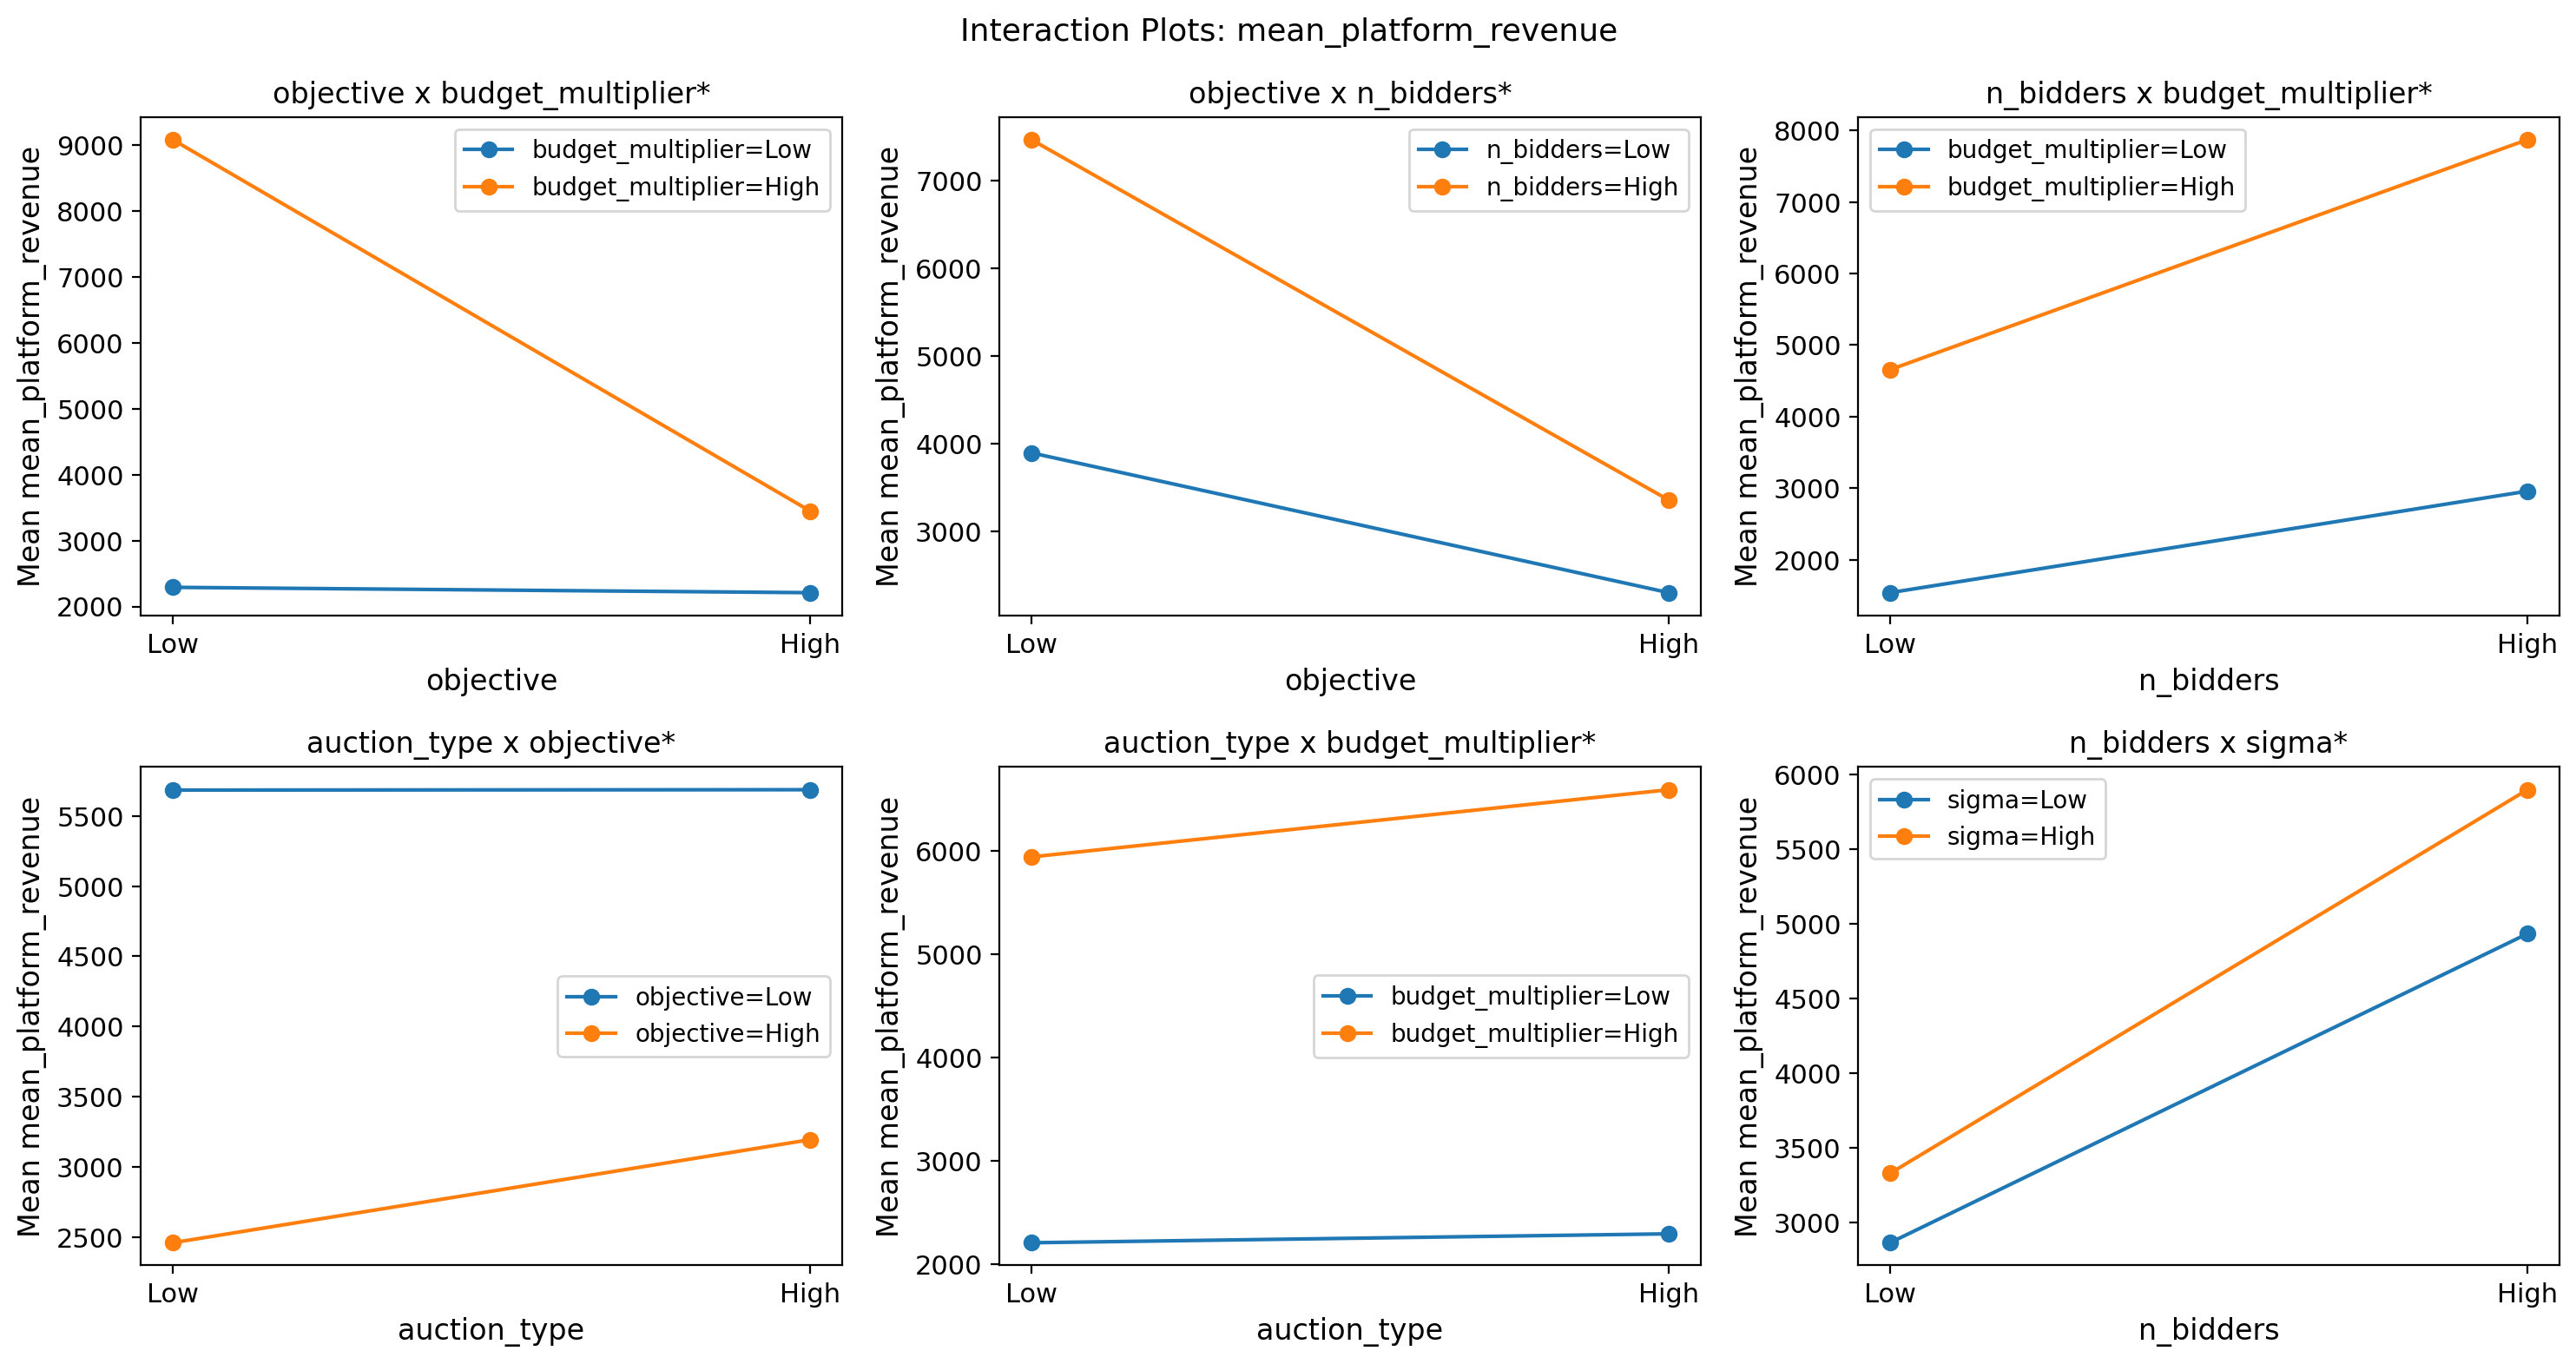
\includegraphics[width=0.75\textwidth]{e3a_int_rev}
\caption{Experiment~3a two-way interactions for platform revenue. The budget multiplier interacts strongly with bidder objective and the number of bidders.}
\label{fig:e3a_int_rev}
\end{figure}

\subsection{Price of Anarchy}

The factorial model for effective Price of Anarchy achieves $R^2 = \ExpThreeAPoaRsq$. \Cref{tab:exp3a_ranked_poa} lists the significant effects.

\begin{table}[H]
\centering
\caption{Experiment 3a: Significant effects for effective Price of Anarchy ($p < 0.05$), ranked by $|t|$.}
\label{tab:exp3a_ranked_poa}
\begin{tabular}{lrrl}
\toprule
\textbf{Effect} & \textbf{Coeff.} & \textbf{$|t|$} & \textbf{Direction} \\
\midrule
Bidder objective $\times$ Budget multiplier & -0.0301 & 17.59 & $-$ \\
Bidder objective & -0.0205 & 12.01 & $-$ \\
Number of bidders & 0.0201 & 11.76 & + \\
Value dispersion ($\sigma$) & -0.0182 & 10.63 & $-$ \\
Budget multiplier & 0.0149 & 8.69 & + \\
Number of bidders $\times$ Value dispersion ($\sigma$) & -0.0142 & 8.28 & $-$ \\
Bidder objective $\times$ Number of bidders & -0.0042 & 2.48 & $-$ \\
Bidder objective $\times$ Value dispersion ($\sigma$) & 0.0039 & 2.29 & + \\
\bottomrule
\end{tabular}
\end{table}


Every observed Price of Anarchy value remains within the theoretical bound $\mathrm{PoA} \leq 2$ derived by \citet{Aggarwal2019} and \citet{Gaitonde2023}. This is a non-trivial confirmation, since the theoretical bound covers worst-case instances and could fail in practice if the pacing dynamics hit a pathological corner of the design space. Auction format does not have a significant main effect on the Price of Anarchy in Experiment~3a, even though it does affect revenue. The pattern that appears in the data is therefore that first-price auctions yield lower seller revenue relative to second-price without a corresponding change in measured allocative efficiency. I report this co-occurrence and do not claim that the one causes the other, since the black-box framing of the thesis does not permit statements about mechanism.

\subsection{Cross-Episode Drift}

\citet{PaesLeme2024} conjecture that dual-based pacing produces progressive bid suppression across campaign cycles. I test this by estimating the slope of the bid-to-value ratio across post-burn-in episodes and relating it to the factorial design. The drift model is statistically significant with an $F$-test $p$-value $\ExpThreeADriftFPFmt$, but the $R^2$ is only $\ExpThreeADriftRsq$ and all cell-level drift estimates remain near zero. The data therefore do not support the direction of the \citet{PaesLeme2024} prediction in this specific discrete-time environment with finite horizons. I do not speculate about whether the theoretical prediction would be recovered under different simulation parameters.

\subsection{Summary of Experiment~3a}

Budget tightness dominates every aspect of dual pacing. The auction-format effect flips sign relative to the learning experiments, though it remains of secondary magnitude. The Price of Anarchy bound holds uniformly. Robustness checks reported in Appendix~\ref{ch:robustness} confirm these findings across all thirteen diagnostic tests.

\section{PI Controller Pacing}
\label{sec:exp3b_results}

Experiment~3b replaces the multiplicative dual update with a PI controller. The agent tracks the cumulative spending error and adjusts its bid-scaling multiplier $\lambda$ through proportional and integral terms; the derivative term is omitted. Aggressiveness is the sixth design factor and controls how reactive the controller is to spending error. \Cref{fig:e3b_trace} shows a representative trajectory.

\begin{figure}[H]
\centering
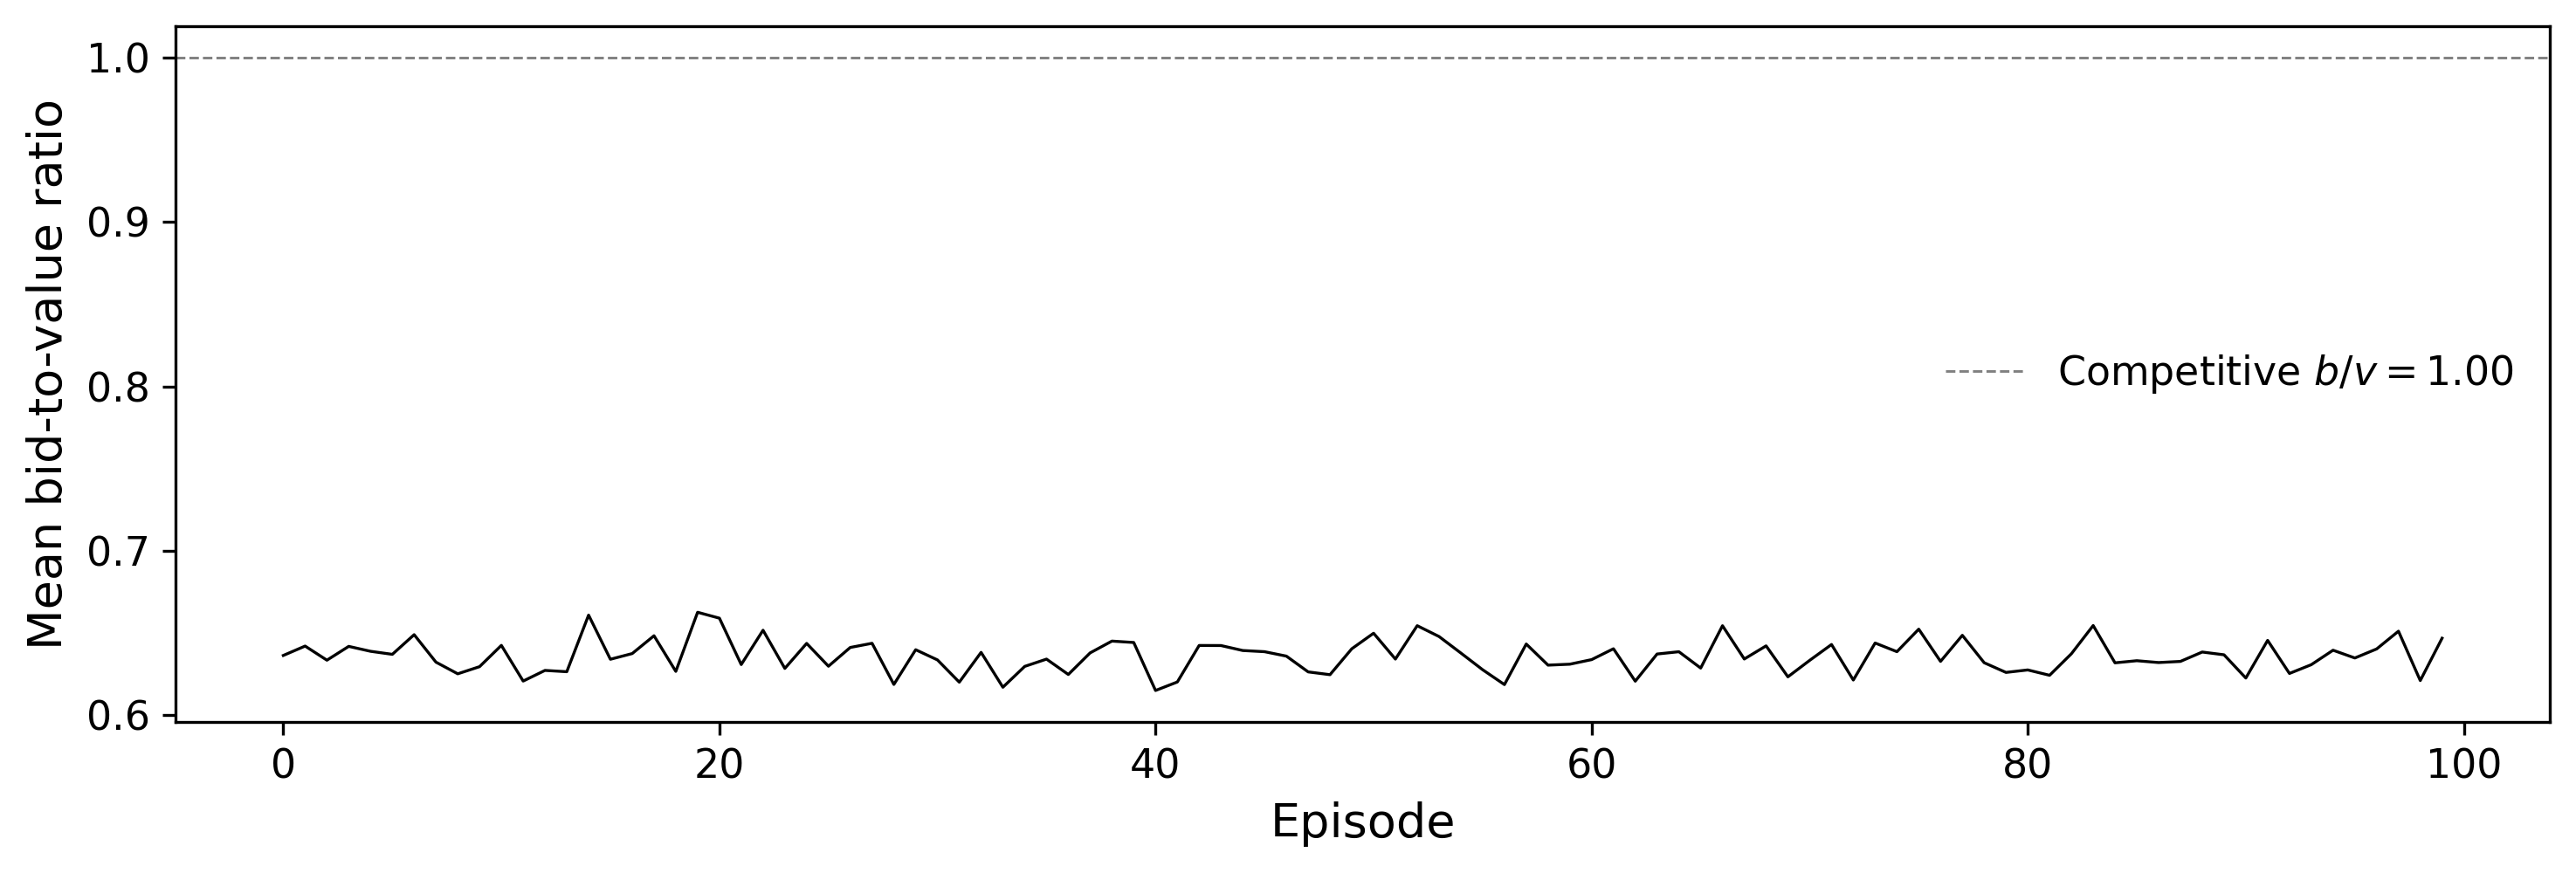
\includegraphics[width=0.75\textwidth]{e3b_trace}
\caption{Representative Experiment~3b trajectory. The plot shows the mean bid-to-value ratio per episode for a single trial with a first-price auction, default aggressiveness, and two bidders.}
\label{fig:e3b_trace}
\end{figure}

\subsection{Revenue}

The budget multiplier again dominates with $|t| = \ExpThreeBRevFactorTOne$ and an effect of \ExpThreeBRevTopPctEffect{} percent of the grand mean. \Cref{tab:exp3b_ranked_rev} lists the significant effects.

\begin{table}[H]
\centering
\caption{Experiment 3b: Significant effects for average revenue ($p < 0.05$), ranked by $|t|$.}
\label{tab:exp3b_ranked_rev}
\begin{tabular}{lrrl}
\toprule
\textbf{Effect} & \textbf{Coeff.} & \textbf{$|t|$} & \textbf{Direction} \\
\midrule
Budget multiplier & 1316.1821 & 31.68 & + \\
Number of bidders & 667.7779 & 16.07 & + \\
Auction format & 458.3301 & 11.03 & + \\
Auction format $\times$ Budget multiplier & 393.6340 & 9.47 & + \\
Value dispersion ($\sigma$) & 360.6121 & 8.68 & + \\
Auction format $\times$ Value dispersion ($\sigma$) & 233.6535 & 5.62 & + \\
Budget multiplier $\times$ Value dispersion ($\sigma$) & 175.0143 & 4.21 & + \\
Number of bidders $\times$ Value dispersion ($\sigma$) & 146.9008 & 3.54 & + \\
\bottomrule
\end{tabular}
\end{table}


Auction format is the second-most important main effect ($|t| = \ExpThreeBRevAuctionAbsT$) and remains positive for first-price, so first-price auctions generate higher revenue than second-price under the PI controller as well. The first-price revenue gap is proportionally larger in Experiment~3b than in Experiment~3a. I report this as a between-experiment comparison, since the two experiments differ only in the pacing control law and share every other design feature; I do not claim that any particular agent "switches" control laws.

The auction-format-by-budget interaction is the largest interaction term ($|t| = 9.5$). The first-price revenue advantage is concentrated in loose-budget settings and narrows to near zero when budgets are tight. I report this as an empirical pattern. A plausible reading is that tight budgets leave little room for the format choice to matter because both formats deliver similar outcomes once the budget constraint binds, but I do not test this mechanistic reading. The auction-format-by-value-dispersion interaction ($|t| = 5.6$) shows that higher value dispersion also widens the first-price advantage. \Cref{fig:e3b_int_rev} shows these interactions.

\begin{figure}[H]
\centering

\includegraphics[width=0.75\textwidth]{e3b_int_rev}
\caption{Experiment~3b two-way interactions for platform revenue. Auction format interacts most strongly with the budget multiplier and with value dispersion.}
\label{fig:e3b_int_rev}
\end{figure}

\subsection{Price of Anarchy}

\begin{table}[H]
\centering
\caption[Experiment 3b: Significant effects for effective price of anarchy ($p < 0.05$), ranked by $|t|$]{\textbf{Experiment 3b: Significant effects for effective price of anarchy ($p < 0.05$), ranked by $|t|$.}}
\label{tab:exp3b_ranked_poa}
\begin{tabular}{lrrl}
\toprule
\textbf{Effect} & \textbf{Coeff.} & \textbf{$|t|$} & \textbf{Direction} \\
\midrule
Auction format & 0.0141 & 10.69 & + \\
Number of bidders $\times$ Budget multiplier & -0.0130 & 9.87 & $-$ \\
Auction format $\times$ Budget multiplier & 0.0073 & 5.56 & + \\
Value dispersion ($\sigma$) & -0.0064 & 4.84 & $-$ \\
Number of bidders & 0.0039 & 2.93 & + \\
Auction format $\times$ Reserve price & 0.0036 & 2.73 & + \\
Number of bidders $\times$ Reserve price & 0.0031 & 2.35 & + \\
Number of bidders $\times$ Value dispersion ($\sigma$) & -0.0029 & 2.21 & $-$ \\
Budget multiplier $\times$ Reserve price & -0.0029 & 2.18 & $-$ \\
Reserve price $\times$ Value dispersion ($\sigma$) & 0.0029 & 2.16 & + \\
\bottomrule
\end{tabular}
\end{table}


Under the PI controller, auction format becomes the dominant main effect on the Price of Anarchy ($|t| \approx 10.7$), with first-price auctions yielding higher Price-of-Anarchy values, that is, lower measured allocative efficiency, than second-price. This is the opposite pattern from dual pacing, where auction format had no significant main effect on the Price of Anarchy. Since the two experiments share every other design feature, the between-experiment difference is associated with the change in control law rather than with any of the other factors. I state this as a descriptive empirical observation rather than a causal property of the control law itself. As in Experiment~3a, every observed Price of Anarchy remains within the theoretical bound of~2.

\subsection{Summary of Experiment~3b}

The budget multiplier remains the dominant revenue driver under PI control. Auction format has a stronger main effect than under dual pacing and also moves the Price of Anarchy significantly, whereas dual pacing insulated allocative efficiency from the choice of format. Controller aggressiveness has a negligible main effect on revenue, which is consistent with the broader finding that algorithmic tuning parameters matter less than structural market conditions. Robustness checks in Appendix~\ref{ch:robustness} confirm all these effects.

\section{What Budget-Constrained Pacing Establishes}
\label{sec:pacing_summary}

Three patterns carry across both pacing sub-experiments. First, the budget multiplier dominates revenue in both 3a and 3b, with total-order Sobol indices above 0.5 in both cases. Tight budgets lower bids uniformly, while loose budgets let the other design factors matter. Second, the number of bidders continues to matter but is no longer the dominant factor. Competitive thickness still pushes revenue up, but its share of explained variance drops well below what it achieved in the learning experiments. Third, and most consequentially, the auction-format effect on revenue reverses sign. Both pacing experiments report first-price auctions generating strictly higher revenue than second-price, a pattern that contradicts the direction observed under LinUCB and Thompson Sampling.

The reversal is not a small margin. Under LinUCB, first-price revenue is about 19 percent below second-price. Under dual pacing, first-price revenue is about 9 percent above second-price. Under PI pacing, the first-price advantage is larger still and interacts more strongly with budget tightness. No single recommendation about auction format generalises across the algorithm families studied in this thesis. I report the pattern without assigning it a mechanism. The black-box approach of this thesis stops at the observation that different bidding technologies respond differently to the format choice. Chapter~\ref{ch:discussion} returns to this reversal and discusses its implications for platform design.

\chapter{Discussion and Conclusion}
\label{ch:discussion}

This chapter synthesises findings across the six sub-experiments, draws out implications for platform design and competition policy, and closes with the main limitations and a short list of directions for future work. I treat every simulation output as a black-box observation. The discussion therefore compares the observed patterns to theoretical predictions and prior empirical work but does not assign mechanistic explanations to the simulation findings.

\section{Synthesis Across Experiments}
\label{sec:synthesis}

\Cref{tab:cross_exp_summary} gathers the top three revenue drivers, the mean revenue by auction format, and the format gap for each of the six sub-experiments. Two cross-cutting patterns stand out.

\begin{table}[H]
\centering
\caption[Cross-experiment summary of revenue drivers and format effects]{\textbf{Cross-experiment summary of revenue drivers and format effects.} For each experiment, the table reports the top three factors by absolute $t$-statistic on platform revenue, the mean revenue under first-price and second-price formats, and the percentage gap between them defined as $(\mathrm{FPA} - \mathrm{SPA}) / \mathrm{SPA}$.}
\label{tab:cross_exp_summary}
\resizebox{\textwidth}{!}{%
\begin{tabular}{l l l l l c c c}
\toprule
& & \multicolumn{3}{c}{\textbf{Top revenue drivers} ($|t|$)} & \multicolumn{3}{c}{\textbf{Revenue by format}} \\
\cmidrule(lr){3-5} \cmidrule(lr){6-8}
\textbf{Exp} & \textbf{Algorithm} & \textbf{Rank 1} & \textbf{Rank 2} & \textbf{Rank 3} & \textbf{FPA} & \textbf{SPA} & \textbf{Gap (\%)} \\
\midrule
1a & Q-learning constant & \ExpOneARevFactorOne{} (\ExpOneARevFactorTOne) & \ExpOneARevFactorTwo{} (\ExpOneARevFactorTTwo) & \ExpOneARevFactorThree{} (\ExpOneARevFactorTThree) & \ExpOneARevMeanFPA & \ExpOneARevMeanSPA & $\ExpOneARevGapPct$ \\
1b & Q-learning affil.\ & \ExpOneBRevFactorOne{} (\ExpOneBRevFactorTOne) & \ExpOneBRevFactorTwo{} (\ExpOneBRevFactorTTwo) & \ExpOneBRevFactorThree{} (\ExpOneBRevFactorTThree) & \ExpOneBRevMeanFPA & \ExpOneBRevMeanSPA & $\ExpOneBRevGapPct$ \\
2a & LinUCB & \ExpTwoARevFactorOne{} (\ExpTwoARevFactorTOne) & \ExpTwoARevFactorTwo{} (\ExpTwoARevFactorTTwo) & \ExpTwoARevFactorThree{} (\ExpTwoARevFactorTThree) & \ExpTwoARevMeanFPA & \ExpTwoARevMeanSPA & $\ExpTwoARevGapPct$ \\
2b & Thompson & \ExpTwoBRevFactorOne{} (\ExpTwoBRevFactorTOne) & \ExpTwoBRevFactorTwo{} (\ExpTwoBRevFactorTTwo) & \ExpTwoBRevFactorThree{} (\ExpTwoBRevFactorTThree) & \ExpTwoBRevMeanFPA & \ExpTwoBRevMeanSPA & $\ExpTwoBRevGapPct$ \\
3a & Dual pacing & \ExpThreeARevFactorOne{} (\ExpThreeARevFactorTOne) & \ExpThreeARevFactorTwo{} (\ExpThreeARevFactorTTwo) & \ExpThreeARevFactorThree{} (\ExpThreeARevFactorTThree) & \ExpThreeARevMeanFPA & \ExpThreeARevMeanSPA & $\ExpThreeARevGapPct$ \\
3b & PI pacing & \ExpThreeBRevFactorOne{} (\ExpThreeBRevFactorTOne) & \ExpThreeBRevFactorTwo{} (\ExpThreeBRevFactorTTwo) & \ExpThreeBRevFactorThree{} (\ExpThreeBRevFactorTThree) & \ExpThreeBRevMeanFPA & \ExpThreeBRevMeanSPA & $\ExpThreeBRevGapPct$ \\
\bottomrule
\end{tabular}}
\end{table}

The first pattern is that structural market parameters rank above algorithmic hyperparameters in every experiment. In the four unconstrained learning experiments, the number of bidders is the top factor for revenue in every case. In the two pacing experiments, the budget multiplier replaces it as the top factor, and the number of bidders drops to third or fourth place. Within each family, learning rates, discount factors, regularisation, memory decay, exploration intensity, and controller aggressiveness all fail to produce significant main effects on revenue at the magnitudes reached by competitive pressure or budget tightness. This empirical ranking points in the same direction as the classical result of \citet{BulowKlemperer1996}, who argue that adding one more bidder matters more than mechanism optimisation in static auctions. I stop short of claiming the two findings are equivalent, since their setting is a one-shot auction with rational bidders and mine is a repeated auction with algorithms, but the directional agreement is worth noting.

The second pattern is that the sign of the auction-format effect on revenue differs between the learning family and the pacing family. Under Q-learning with constant valuations, the two formats generate nearly identical revenue. Under Q-learning with affiliated valuations and under both contextual-bandit experiments, second-price auctions generate higher revenue, with format gaps of roughly 11, 19, and 9 percent respectively. Under both pacing experiments, first-price auctions generate higher revenue, with format gaps of roughly 9 percent under dual pacing and a larger positive gap under PI pacing. The between-family sign difference is not a small margin, and it holds under every robustness check reported in \cref{ch:robustness}. The format ranking that \citet{BanchioSkrzypacz2022} report from Q-learning experiments, in which first-price auctions appear more vulnerable to bid suppression than second-price, does not carry over to the pacing family in my simulations, where the opposite direction holds.

The two patterns combine into a single message for auction designers. A platform asking whether it should use first-price or second-price formats cannot read a universal recommendation off the economic-theory shelf, nor off the reinforcement-learning literature, nor off the autobidding literature. The ordering depends on the bidding technology the agents actually use. If a platform's advertisers deploy budget-constrained pacing systems similar to the ones I study, my simulation output would recommend first-price formats; if they run unconstrained learning algorithms with affiliated signals similar to mine, it would recommend second-price. Platforms running both kinds of agents face a trade-off that my experiments cannot resolve on their own, since the thesis studies each algorithm family in isolation and does not simulate mixed populations.

\section{Policy Implications}
\label{sec:policy}

Two implications follow for competition policy, subject to the caveat that both are drawn from simulation output and depend on the external validity of the laboratory. The first is that the factor with the largest measured effect on seller revenue, in every experiment of this thesis, is structural. The number-of-bidders factor ranks first in every learning experiment, and the budget multiplier ranks first in every pacing experiment. Algorithmic tuning factors never match their magnitudes. If that ranking carries over to real markets, interventions that raise the number of active bidders or that loosen budget constraints would do more for revenue than any of the algorithmic or format-based interventions I vary in the factorial designs. The corresponding policy ideas, lowering barriers to entry, preventing excessive buyer concentration, and avoiding restrictive spend caps, are ordinary structural remedies and my results give them the same directional support they already have in classical auction theory \citep{BulowKlemperer1996}.

The second implication is that format-based regulation faces a heterogeneity problem. A rule that mandates one auction format as safer than the other requires that the format ranking be stable across the bidding technologies regulators will actually encounter. My findings in \crefrange{ch:qlearning}{ch:pacing} show that, within the settings I study, it is not. A rule favouring second-price auctions on the basis of the Q-learning literature would misfire in markets where pacing bidders predominate, and a rule favouring first-price auctions on the basis of the pacing literature would misfire in markets dominated by unconstrained learners. Regulators who wish to address algorithmic bid suppression would need to condition their recommendations on the bidding technology they audit, which is harder than issuing a blanket rule. Outcome-based monitoring, in which the regulator looks at realised revenue shortfalls rather than the choice of format, sits more comfortably with this heterogeneity. \citet{Hartline2024} propose regret auditing in the same spirit, where algorithmic bidders are evaluated against the performance they could have achieved with the best fixed action rather than against claims about intent.

A related implication concerns the evidentiary threshold for antitrust liability. Both United States antitrust law and European competition law require evidence of agreement or concerted practice to establish liability for horizontal coordination, and no jurisdiction has yet sanctioned purely autonomous tacit collusion by independent learning algorithms \citep{EzrachiStucke2017, Mehra2016}. The factorial laboratory supplies one ingredient that such sanctions would need, which is a transparent and reproducible ranking of the design factors associated with revenue shortfalls, along with direction, magnitude, and statistical significance. A regulator could in principle require platforms to run standardized factorial experiments on their own bidding systems and report the ranked effects, or could construct a parallel laboratory independently. The ranked-effects tables and Sobol decompositions in this thesis illustrate the kind of output that such a compliance exercise would deliver. Whether any jurisdiction would in fact adopt this approach is a separate question that my experiments do not address.

\section{Limitations}
\label{sec:limitations}

The experiments are stylised. The bidder populations are small, symmetric, and drawn from a handful of value models. The algorithms are tabular Q-learning, linear contextual bandits, and two pacing variants; they do not include deep reinforcement learning, transformer-based bidders, or large-language-model agents. There is no explicit communication channel between bidders, no combinatorial allocation, no auction-revenue feedback into bidder populations, and no entry or exit dynamics. Episode lengths are fixed and burn-in periods are standardised. The log-normal valuation model in the pacing experiments is specifically chosen to mirror the stylised setting of the autobidding literature and is not calibrated to any real exchange. External validity to a specific market requires empirical validation with proprietary auction data, which I do not have.

The black-box framing is both a strength and a limitation. It disciplines the interpretation of results, since I report only what the input-output map shows, but it leaves unanswered the mechanistic question of why the observed patterns arise. I cannot tell whether the auction-format reversal under pacing is driven by the dual-update dynamics, the budget cap, the pacing feedback loop, or some interaction among these features. Mechanistic investigations using either analytical pacing theory or targeted ablations would complement the black-box diagnosis.

Finally, the factorial design spans a fixed set of factor levels. The rankings are valid within the ranges tested. Extreme misconfigurations, such as near-zero learning rates, implausibly large budgets, or a single dominant bidder with monopsony power, could change the ordering, but those cases are unlikely to represent any real market of economic interest.

\section{Future Directions}
\label{sec:future}

Three extensions seem particularly worthwhile. The first is to apply the same factorial framework to deep reinforcement-learning agents (neural networks trained to bid by trial and error) and to large-language-model bidders (systems that receive prompts and return bid decisions), since these are the technologies most likely to be deployed in newly developed auction markets. A replication of the format-reversal result with these algorithm families would considerably strengthen its policy relevance. The second is to move from screening designs, which identify which factors matter, to response-surface designs, which trace out the functional relationship between the factors that matter and the outcome. Knowing the shape of the relationship between the number of bidders, the budget multiplier, and revenue would allow a platform to set quantitative targets rather than simply prefer one direction to another. The third is to seek empirical validation on real auction data. Several major advertising exchanges run internal shadow experiments and factor tests, and cooperation with such a platform would let the black-box framework confront real bidding populations and check whether the laboratory rankings replicate in production.

The computational laboratory developed in this thesis offers a standardised pipeline for auction platforms and antitrust regulators who want to diagnose algorithmic behaviour without committing themselves to any particular theory of how the algorithms generate their outputs. The pipeline is portable, the analysis is mechanical, and the outputs are transparent. I hope it proves useful beyond the specific experiments reported here.

\section{A Short Plain-Language Summary}
\label{sec:plain_summary}

If I had to summarise the thesis in three sentences for a reader who wanted the economic point without the statistical machinery, they would be the following. When bidders are algorithms rather than humans, the auctioneer's revenue is shaped far more by the market's structural features (how many bidders compete and how tight their budgets are) than by the choices the algorithms' designers make about learning rates, exploration schedules, or update rules. The choice between first-price and second-price auctions does not have a universal ranking. Second-price formats raise more revenue when bidders are unconstrained learners, and first-price formats raise more revenue when bidders are budget-constrained pacers. A policy recommendation that works well for one class of algorithms can therefore be the wrong recommendation for another, and regulators, platforms, and auction designers should condition their choices on the bidding technology that actually populates the market.


\bibliographystyle{plainnat}
\bibliography{references}

\appendix
\chapter{Equilibrium Benchmarks}
\label{ch:equilibria}

This appendix derives the rational-bidder equilibrium benchmarks that the results chapters compare against. The derivations are standard and are collected here to keep the main text focused on the experimental findings.

\section{Constant Valuations}
\label{sec:eq_constant}

Experiment~1a uses constant valuations $v_i = 1$ with the discrete bid grid $\mathcal{B} = \{0, 0.1, \ldots, 1.0\}$. In a first-price auction with $n$ bidders, a symmetric profile in which every bidder bids $b$ yields each bidder an expected payoff of $(1 - b) / n$, since ties are broken uniformly at random. A unilateral upward deviation to $b + 0.1$ (provided $b + 0.1 \leq 1$) yields a payoff of $1 - (b + 0.1)$. No upward deviation is profitable when
\[
1 - (b + 0.1) \;\leq\; \frac{1 - b}{n},
\]
which after rearrangement gives
\[
b \;\geq\; \frac{0.9\,n - 1}{n - 1}.
\]
For any $b$ at or above this threshold and bounded by the grid, the symmetric profile is a pure-strategy Nash equilibrium. With $n = 2$ the threshold is $0.8$, and with $n = 4$ the threshold is approximately $0.87$.

In a second-price auction with identical valuations, bidding $v_i = 1$ is weakly dominant, since the winner pays the second-highest bid regardless of her own bid. Any profile in which at least one bidder bids $1$ is a Nash equilibrium, and the expected revenue to the seller is $1$. Under revenue equivalence \citep{Vickrey1961} the two formats deliver the same expected revenue, so the first-price equilibrium threshold derivation above pins down the minimum symmetric bid consistent with non-dominated play.

\section{Affiliated Valuations}
\label{sec:eq_affiliated}

Experiments~1b, 2a, and 2b use the linear-affiliation model of \Cref{sec:env}. Each bidder draws a signal $s_i$ uniformly on $\{0, 0.1, \ldots, 1.0\}$, and her valuation is
\[
v_i \;=\; \alpha \, s_i \;+\; \beta \sum_{j \neq i} s_j,
\qquad
\alpha = 1 - \frac{\eta}{2},
\qquad
\beta = \frac{\eta}{2 (n - 1)},
\]
with $\eta \in \{0, 0.5, 1\}$. Signals are drawn independently across bidders and rounds. The symmetric Bayes-Nash equilibrium in both formats features a linear bid function.

\subsection{Bid Functions}

In the second-price auction with independent private values, each bidder has a dominant strategy to bid her expected valuation conditional on the event that she ties for the highest bid. Under the linear model above, the resulting symmetric bid function is
\[
b^{\mathrm{SPA}}(s) \;=\; \Big(\alpha + \frac{n \beta}{2}\Big) s.
\]
The derivation conditions on the highest rival signal equalling the bidder's own signal. Her own signal contributes $\alpha s$, the tying rival contributes $\beta s$, and each of the remaining $n - 2$ rivals contributes $\beta \, \mathbb{E}[s_j \mid s_j \leq s] = \beta s / 2$. Summing across the $n - 1$ rival contributions gives $\beta (1 + (n-2)/2) s = \beta (n/2) s$, which yields the formula above.

In the first-price auction under independent uniform signals, the standard envelope argument produces
\[
b^{\mathrm{FPA}}(s) \;=\; \frac{n - 1}{n} \Big(\alpha + \frac{n \beta}{2}\Big) s.
\]
The bid function is linear in the signal, with a shading factor $(n - 1)/n$ that captures the first-price markdown.

\subsection{Expected Revenue}

Let $\phi = \alpha + n \beta / 2$. Under independent uniform signals on $[0, 1]$, the highest signal has expected value $n / (n + 1)$ and the second-highest signal has expected value $(n - 1) / (n + 1)$. Expected revenue in each format is the bid slope times the relevant order statistic, which gives
\[
R^{\mathrm{SPA}} \;=\; \phi \cdot \frac{n - 1}{n + 1},
\qquad
R^{\mathrm{FPA}} \;=\; \frac{n - 1}{n} \cdot \phi \cdot \frac{n}{n + 1} \;=\; \phi \cdot \frac{n - 1}{n + 1}.
\]
The two expressions coincide, so revenue equivalence holds for every affiliation level $\eta$ in this model. The equivalence holds because signals are drawn independently, which is why the classical \citet{MilgromWeber1982} ranking in favour of second-price formats does not apply here; their ranking requires positively affiliated signals in the strict technical sense. The linear-affiliation function I use creates interdependent valuations but preserves signal independence.

\subsection{Efficient Benchmark}

The expected value of the highest valuation is
\[
\mathbb{E}[v_{(1)}] \;=\; (\alpha - \beta) \, \mathbb{E}[s_{(1:n)}] \;+\; \beta \, \mathbb{E}[S],
\]
where $s_{(1:n)}$ is the maximum of $n$ independent uniform signals and $S = \sum_i s_i$. Substituting $\mathbb{E}[s_{(1:n)}] = n / (n + 1)$ and $\mathbb{E}[S] = n / 2$, the expression simplifies to
\[
\mathbb{E}[v_{(1)}] \;=\; (\alpha - \beta) \cdot \frac{n}{n + 1} \;+\; \beta \cdot \frac{n}{2}.
\]
This is the efficient first-best benchmark. The factorial analysis in Chapter~\ref{ch:qlearning} reports realised revenues rather than welfare, so the efficient benchmark enters the discussion only for comparison with the Price of Anarchy analysis in Chapter~\ref{ch:pacing}.

\section{Numerical Verification}
\label{sec:eq_numerical}

The analytical equilibria above are verified by numerical simulation. The deviation check fixes a grid of signal types and computes the expected payoff from multiplicative deviations around the predicted equilibrium bid. \Cref{tab:bne_deviation} reports the maximal gain from deviating for each $(\eta, n)$ pair; values at numerical zero indicate that the proposed bid is a best response at the reported precision.

\begin{table}[H]
  \centering
  \small
  \caption{Maximum payoff gain from unilateral deviation. Values near zero confirm BNE optimality (200K MC draws per configuration).}
  \label{tab:bne_deviation}
  \begin{tabular}{ccccc}
    \toprule
    $\eta$ & $N$ & Auction & Bid slope & Max Gain \\
    \midrule
    0.0 & 2 & FIRST & 0.5000 & 0.000000 \\
    0.0 & 2 & SECOND & 1.0000 & 0.000000 \\
    0.0 & 3 & FIRST & 0.6667 & 0.000129 \\
    0.0 & 3 & SECOND & 1.0000 & 0.000000 \\
    0.0 & 6 & FIRST & 0.8333 & 0.000002 \\
    0.0 & 6 & SECOND & 1.0000 & 0.000000 \\
    0.5 & 2 & FIRST & 0.5000 & 0.000034 \\
    0.5 & 2 & SECOND & 1.0000 & 0.000000 \\
    0.5 & 3 & FIRST & 0.6250 & 0.000024 \\
    0.5 & 3 & SECOND & 0.9375 & 0.000001 \\
    0.5 & 6 & FIRST & 0.7500 & 0.000000 \\
    0.5 & 6 & SECOND & 0.9000 & 0.000000 \\
    1.0 & 2 & FIRST & 0.5000 & 0.000084 \\
    1.0 & 2 & SECOND & 1.0000 & 0.000000 \\
    1.0 & 3 & FIRST & 0.5833 & 0.000020 \\
    1.0 & 3 & SECOND & 0.8750 & 0.000002 \\
    1.0 & 6 & FIRST & 0.6667 & 0.000003 \\
    1.0 & 6 & SECOND & 0.8000 & 0.000000 \\
    \bottomrule
  \end{tabular}
\end{table}

The revenue check runs Monte Carlo simulations at the equilibrium bids and compares realised mean revenue to the closed-form prediction $R^{\mathrm{BNE}} = \phi \cdot (n - 1)/(n + 1)$ for both formats. \Cref{tab:bne_revenue_match} reports the results.

\begin{table}[H]
  \centering
  \small
  \caption[Revenue formula validation: Analytical vs.\ Monte Carlo (500K draws)]{\textbf{Revenue formula validation: Analytical vs.\ Monte Carlo (500K draws).} Revenue equivalence holds under iid signals.}
  \label{tab:bne_revenue_match}
  \begin{tabular}{cccccc}
    \toprule
    $\eta$ & $N$ & $R^{\text{analytical}}$ & $R^{\text{FPA}}_{\text{MC}}$ & $R^{\text{SPA}}_{\text{MC}}$ & $|R^{\text{FPA}} - R^{\text{SPA}}|$ \\
    \midrule
    0.0 & 2 & 0.3333 & 0.3330 & 0.3337 & 0.0007 \\
    0.0 & 3 & 0.5000 & 0.5000 & 0.4997 & 0.0003 \\
    0.0 & 6 & 0.7143 & 0.7145 & 0.7145 & 0.0000 \\
    0.5 & 2 & 0.3333 & 0.3330 & 0.3337 & 0.0007 \\
    0.5 & 3 & 0.4688 & 0.4688 & 0.4685 & 0.0003 \\
    0.5 & 6 & 0.6429 & 0.6431 & 0.6430 & 0.0000 \\
    1.0 & 2 & 0.3333 & 0.3330 & 0.3337 & 0.0007 \\
    1.0 & 3 & 0.4375 & 0.4375 & 0.4372 & 0.0003 \\
    1.0 & 6 & 0.5714 & 0.5716 & 0.5716 & 0.0000 \\
    \bottomrule
  \end{tabular}
\end{table}

The Monte Carlo means match the closed-form predictions within tight confidence intervals, and the first-price and second-price revenues coincide within sampling error, confirming revenue equivalence.

\section{Pacing Equilibrium}
\label{sec:eq_pacing}

The pacing experiments in Chapter~\ref{ch:pacing} do not admit a closed-form Bayes-Nash benchmark, because budget constraints couple the bidder's choices across rounds. Instead, the relevant equilibrium concept is the first-price pacing equilibrium introduced by \citet{Conitzer2022FPPE}, which is unique under mild regularity conditions and computable via the Eisenberg-Gale convex programme. The welfare benchmark is the liquid welfare optimum defined in \Cref{sec:welfare}, and the efficiency benchmark is the Price of Anarchy bound of $\mathrm{PoA} \leq 2$ derived by \citet{Aggarwal2019} and \citet{Gaitonde2023}. I do not rederive these results here; the reader is referred to the original sources for the full constructions.

\chapter{Robustness and Model Adequacy}
\label{ch:robustness}

This appendix collects the robustness and model-adequacy diagnostics that support the findings reported in the results chapters. I group the checks by what they test rather than parade them one by one. The main body reports that the dominant factor rankings survive all of these diagnostics; this appendix provides the supporting detail.

\section{Model Adequacy}
\label{sec:app_adequacy}

Model adequacy is assessed by four complementary diagnostics. Each addresses a distinct failure mode of the linear main-effects-plus-two-way-interactions specification.

The first diagnostic is the in-sample $R^2$ of the OLS model. Across all six sub-experiments, the $R^2$ for platform revenue ranges from $\ExpOneBRevRsq$ in Experiment~1b to $\ExpThreeARevRsq$ in Experiment~3a. The highest $R^2$ values are recorded under pacing, where the outcome is more tightly determined by the budget and design structure; the lowest are recorded under contextual bandits and Q-learning with affiliated signals, where additional seed-level variability enters through the stochastic exploration mechanism.

The second diagnostic is the out-of-sample $R^2$ computed via the predicted residual error sum of squares (PRESS) statistic. PRESS is a closed-form way to compute leave-one-out cross-validation for an OLS regression. It uses the hat matrix of the fit rather than actually refitting the model after removing each observation, so the answer is identical to leave-one-out cross-validation but cheaper. The gap between in-sample $R^2$ and leave-one-out cross-validated $R^2$ is below 0.10 for every response variable in every sub-experiment, with the largest gap recorded in Experiment~1b ($\ExpOneBRevPRESSGap$) and the smallest in Experiment~3a ($\ExpThreeARevPRESSGap$). A gap below 0.10 indicates that the linear model generalises cleanly and does not overfit the design.

The third diagnostic benchmarks the linear model against a gradient-boosted tree ensemble (LightGBM) fit with five-fold cross-validation. LightGBM can approximate arbitrary nonlinear interactions given enough data, so its cross-validated $R^2$ provides a nonparametric upper bound on how much signal the data contain. In Experiments~1b, 2b, 3a, and 3b, LightGBM's cross-validated $R^2$ is comparable to or lower than OLS $R^2$, which means the linear specification captures essentially all the signal. In Experiments~1a and~2a, LightGBM's cross-validated $R^2$ modestly exceeds OLS $R^2$ for one or two responses, indicating mild nonlinearity that the linear model does not capture. The dominant factor rankings are unchanged when the analysis is rerun with a LightGBM feature-importance ranking.

The fourth diagnostic is a lack-of-fit $F$-test. The test exploits the within-cell replication of the factorial designs to decompose the residual sum of squares into two pieces: pure error (the variance of replicate runs within the same design cell) and lack of fit (the deviation of cell means from the model's predicted cell means). If the second piece is large relative to the first, the linear model is missing systematic structure. Lack of fit is detectable but small for all experiments, and the dominant effects retain their ranking when the model is extended to include three-way interactions.

\section{Multiple Testing}
\label{sec:app_multiple_testing}

Each experiment reports many effect estimates simultaneously, so I apply two multiple-testing corrections. The Holm step-down procedure controls the family-wise error rate at $\alpha = 0.05$, and the Benjamini-Hochberg procedure controls the false-discovery rate at the same level. Rademacher wild-bootstrap $p$-values are also computed for the top ten effects of each response variable to guard against distributional misspecification, with 1000 iterations per test.

Across all six sub-experiments, the effects I report as significant in the main text survive both Holm and Benjamini-Hochberg. The fraction of effects surviving Benjamini-Hochberg varies across experiments, ranging from $\ExpOneBBHPct$ percent in Experiment~1b to $\ExpThreeABHPct$ percent in Experiment~3a. Wild-bootstrap $p$-values align closely with asymptotic HC3 $p$-values, with differences below 0.01 in every case. HC3 heteroskedasticity-consistent standard errors change the significance status of at most 2.1 percent of effects (recorded in Experiment~2b) across the six sub-experiments, so the conclusions are not driven by the choice between classical OLS and HC3 standard errors.

\section{Quantile Regression}
\label{sec:app_quantile}

The OLS analysis conditions on the mean of the response. Some factors may have effects that are concentrated in the tails of the outcome distribution and are therefore invisible to mean regression. I fit quantile regressions at the 10th, 25th, 50th, 75th, and 90th percentiles for platform revenue in each sub-experiment, using the Holm step-down correction across the full family of factor-by-quantile tests.

The most striking quantile finding is in Experiment~1a, where the auction-format coefficient reverses sign across quantiles. At the 10th percentile of revenue, first-price auctions raise revenue by roughly $+0.033$, and at the 90th percentile they lower it by roughly $-0.047$, with the crossover between the median and the 75th percentile. Both tails are significant under Holm correction, and both effects disappear when averaged into the OLS mean regression. First-price auctions therefore compress the revenue distribution, raising the floor and lowering the ceiling, even though they have no significant main effect on the conditional mean. This sign reversal is a distributional pattern that OLS masks by construction.

In Experiments~2b, 3a, and 3b, the auction-format effect grows monotonically towards the upper tail of the revenue distribution rather than reversing sign. The first-price penalty under Thompson Sampling nearly doubles from the 10th percentile to the 90th, and the first-price advantage under PI pacing nearly doubles in the same direction. The best-performing configurations are the most sensitive to the choice of auction format in both directions. The number-of-bidders effect is stable across quantiles in every experiment, confirming that market thickness benefits revenue uniformly.

\section{LASSO Variable Selection}
\label{sec:app_lasso}

The LASSO estimator of \citet{Tibshirani1996} simultaneously estimates coefficients and selects variables through an $L_1$ penalty that shrinks small coefficients exactly to zero. I fit LASSO models for each response variable in each experiment, with the regularisation parameter $\lambda$ chosen by five-fold cross-validation to minimise mean squared error. I then check whether the LASSO-surviving variables match the OLS-significant variables.

LASSO retains auction format and the number of bidders in every sub-experiment. No interaction survives LASSO whose parent main effects were dropped, so the LASSO fit respects the effect-heredity principle that interactions should only be retained when their constituent main effects are also present. The LASSO-selected variables are a subset of the OLS-significant effects in every case, with LASSO being more conservative as expected under the $L_1$ penalty.

\section{Discretisation and Budget Sensitivity}
\label{sec:app_sensitivity}

Two external sensitivity checks probe whether the findings depend on specific parameter choices. The first is a discretisation sensitivity analysis for Experiments~1a through 2b. I rerun a representative subset of factorial cells at bid-grid sizes of 6, 11, and 21 discrete levels. The dominant factor rankings are stable across grid sizes, and the relative ordering of the top effects is preserved at every granularity. Mean response values shift modestly as the grid coarsens, consistent with approximation error proportional to the grid spacing, but no effect changes sign or significance.

The second is a budget sensitivity analysis for Experiment~3a. I rerun the pacing design with budget multipliers $m \in \{0.25, 0.5, 1.0\}$. Tighter budgets amplify the bidder-objective effect on revenue, while looser budgets reduce the auction-format effect because the pacing constraint becomes less binding. The number of bidders remains the dominant factor at every budget level. The auction-format reversal between pacing and learning experiments survives across all three budget levels.

\section{Sobol Sensitivity Methods}
\label{sec:app_sobol}

The analytical Sobol decomposition in \Cref{sec:sensitivity_main} is supplemented by six alternative sensitivity methods. Random-forest permutation importance measures how much the test-set accuracy of a random-forest fit drops when a given factor is randomly shuffled. SHAP (Shapley additive explanation) values decompose the prediction of a machine-learning model into an additive contribution from each feature, using a weighting drawn from cooperative game theory. Morris elementary effects average the finite-difference contribution of each factor along randomised one-step perturbation paths through the design space. Monte Carlo Sobol indices estimate the same variance decomposition as the analytical indices, but by sampling from surrogate models (I use a neural network, the gradient-boosted tree ensemble, and a Kriging interpolator, which is a Gaussian-process regression model named after the mining engineer D.\ G.\ Krige). FAST (Fourier amplitude sensitivity test) uses Fourier analysis to separate the contribution of each factor to output variance. Borgonovo's $\delta$ measure is a moment-independent sensitivity indicator that captures how much the distribution of the output shifts when a factor is fixed at its mean. Each method returns an importance score per factor, and I compute the pairwise Spearman rank correlation between methods within each experiment and response to assess concordance.

Cross-method concordance is strong in the experiments with clear dominant factors and large sample sizes. Experiment~1a records a mean Spearman correlation of 0.87 across all methods and responses, and Experiments~3a and~3b record correlations of 0.72 and 0.77 respectively. Concordance is weaker in Experiments~2a and~2b, where many factors have similar importance and the methods disagree on the ordering of minor effects, though the identity of the top one or two factors remains consistent across methods.

\section{Summary}
\label{sec:app_summary}

The robustness analysis supports three claims that recur throughout the results chapters. First, the dominant factor rankings are stable under multiple-testing correction, distributional-assumption-free inference, quantile regression at five percentiles, LASSO variable selection, discretisation sensitivity, budget sensitivity, and six alternative sensitivity methods. Second, model adequacy is high across the board, with linear $R^2$ close to the nonparametric benchmark and leave-one-out cross-validated gaps below 0.10 in every experiment. Third, distributional heterogeneity exists for the auction-format effect and is invisible to standard OLS at the conditional mean; quantile regression uncovers it in Experiment~1a as a sign reversal across percentiles, and in Experiments~2b, 3a, and 3b as a monotone growth towards the upper tail.

\chapter{Ranked-Effects Tables}
\label{ch:ranked_tables}

This appendix collects the ranked-effects tables for all six sub-experiments, listing significant effects ordered by absolute $t$-statistic for each primary response variable. The main text summarises the key patterns; the full coefficient rankings appear below.

\section{Q-Learning Experiments}

\subsection{Experiment~1a: Constant Valuations}

\begin{table}[H]
\centering
\caption{Experiment 1a: Significant effects for average revenue ($p < 0.05$), ranked by $|t|$.}
\label{tab:exp1a_ranked_rev}
\begin{tabular}{lrrl}
\toprule
\textbf{Effect} & \textbf{Coeff.} & \textbf{$|t|$} & \textbf{Direction} \\
\midrule
Number of bidders & 0.0871 & 17.75 & + \\
Discount factor ($\gamma$) & -0.0453 & 9.23 & $-$ \\
Update mode & 0.0366 & 7.45 & + \\
Discount factor ($\gamma$) $\times$ Number of bidders & 0.0298 & 6.09 & + \\
Auction format $\times$ Number of bidders & -0.0276 & 5.63 & $-$ \\
Reserve price & 0.0250 & 5.10 & + \\
Reserve price $\times$ Information feedback & -0.0219 & 4.47 & $-$ \\
Auction format $\times$ Discount factor ($\gamma$) & -0.0215 & 4.38 & $-$ \\
Auction format $\times$ Update mode & -0.0193 & 3.94 & $-$ \\
Information feedback & 0.0182 & 3.71 & + \\
\bottomrule
\end{tabular}
\end{table}


\subsection{Experiment~1b: Affiliated Valuations}

\begin{table}[H]
\centering
\caption[Experiment 1b: significant effects for average revenue ($p < 0.05$), ranked by $|t|$]{\textbf{Experiment 1b: significant effects for average revenue ($p < 0.05$), ranked by $|t|$.}}
\label{tab:exp1b_ranked_rev}
\begin{tabular}{lrrl}
\toprule
\textbf{Effect} & \textbf{Coeff.} & \textbf{$|t|$} & \textbf{Direction} \\
\midrule
Number of bidders & 0.0552 & 6.53 & + \\
State information & -0.0495 & 5.85 & $-$ \\
Auction format $\times$ Number of bidders & -0.0285 & 3.38 & $-$ \\
Auction format & -0.0268 & 3.17 & $-$ \\
Number of bidders $\times$ State information & -0.0263 & 3.11 & $-$ \\
\bottomrule
\end{tabular}
\end{table}


\section{Contextual Bandit Experiments}

\subsection{Experiment~2a: LinUCB}

\begin{table}[H]
\centering
\caption{Experiment 2a: Significant effects for average revenue ($p < 0.05$), ranked by $|t|$.}
\label{tab:exp2a_ranked_rev}
\begin{tabular}{lrrl}
\toprule
\textbf{Effect} & \textbf{Coeff.} & \textbf{$|t|$} & \textbf{Direction} \\
\midrule
Number of bidders & 0.1308 & 33.90 & + \\
Auction format & -0.0482 & 12.49 & $-$ \\
Number of bidders $\times$ Reserve price & -0.0400 & 10.36 & $-$ \\
Auction format $\times$ Number of bidders & -0.0245 & 6.35 & $-$ \\
Reserve price $\times$ Context richness & -0.0223 & 5.78 & $-$ \\
Affiliation (linear) & -0.0135 & 5.71 & $-$ \\
Affiliation (linear) $\times$ Affiliation (quadratic) & -0.0135 & 5.71 & $-$ \\
Exploration intensity & -0.0168 & 4.37 & $-$ \\
Auction format $\times$ Reserve price & 0.0150 & 3.88 & + \\
Exploration intensity $\times$ Context richness & 0.0137 & 3.54 & + \\
\bottomrule
\end{tabular}
\end{table}


\subsection{Experiment~2b: Thompson Sampling}

\begin{table}[H]
\centering
\caption[Experiment 2b: significant effects for average revenue ($p < 0.05$), ranked by $|t|$]{\textbf{Experiment 2b: significant effects for average revenue ($p < 0.05$), ranked by $|t|$.}}
\label{tab:exp2b_ranked_rev}
\begin{tabular}{lrrl}
\toprule
\textbf{Effect} & \textbf{Coeff.} & \textbf{$|t|$} & \textbf{Direction} \\
\midrule
Number of bidders & 0.0525 & 8.69 & + \\
Reserve price & -0.0480 & 7.95 & $-$ \\
Number of bidders $\times$ Context richness & 0.0284 & 4.71 & + \\
Auction format $\times$ Number of bidders & -0.0245 & 4.07 & $-$ \\
Auction format & -0.0231 & 3.83 & $-$ \\
Exploration intensity & -0.0204 & 3.38 & $-$ \\
Affiliation (linear) $\times$ Affiliation (quadratic) & -0.0117 & 3.18 & $-$ \\
Affiliation (linear) & -0.0117 & 3.18 & $-$ \\
Context richness & -0.0175 & 2.89 & $-$ \\
Number of bidders $\times$ Reserve price & -0.0174 & 2.88 & $-$ \\
\bottomrule
\end{tabular}
\end{table}


\section{Budget-Constrained Pacing Experiments}

\subsection{Experiment~3a: Dual Pacing}

\begin{table}[H]
\centering
\caption{Experiment 3a: Significant effects for average revenue ($p < 0.05$), ranked by $|t|$.}
\label{tab:exp3a_ranked_rev}
\begin{tabular}{lrrl}
\toprule
\textbf{Effect} & \textbf{Coeff.} & \textbf{$|t|$} & \textbf{Direction} \\
\midrule
Budget multiplier & 2006.6019 & 39.44 & + \\
Bidder objective & -1428.0108 & 28.07 & $-$ \\
Bidder objective $\times$ Budget multiplier & -1387.4815 & 27.27 & $-$ \\
Number of bidders & 1158.2655 & 22.76 & + \\
Bidder objective $\times$ Number of bidders & -629.6958 & 12.38 & $-$ \\
Number of bidders $\times$ Budget multiplier & 448.9495 & 8.82 & + \\
Value dispersion ($\sigma$) & 356.7849 & 7.01 & + \\
Auction format & 184.0336 & 3.62 & + \\
Auction format $\times$ Bidder objective & 182.7252 & 3.59 & + \\
Auction format $\times$ Budget multiplier & 140.8645 & 2.77 & + \\
\bottomrule
\end{tabular}
\end{table}


\begin{table}[H]
\centering
\caption{Experiment 3a: Significant effects for effective Price of Anarchy ($p < 0.05$), ranked by $|t|$.}
\label{tab:exp3a_ranked_poa}
\begin{tabular}{lrrl}
\toprule
\textbf{Effect} & \textbf{Coeff.} & \textbf{$|t|$} & \textbf{Direction} \\
\midrule
Bidder objective $\times$ Budget multiplier & -0.0301 & 17.59 & $-$ \\
Bidder objective & -0.0205 & 12.01 & $-$ \\
Number of bidders & 0.0201 & 11.76 & + \\
Value dispersion ($\sigma$) & -0.0182 & 10.63 & $-$ \\
Budget multiplier & 0.0149 & 8.69 & + \\
Number of bidders $\times$ Value dispersion ($\sigma$) & -0.0142 & 8.28 & $-$ \\
Bidder objective $\times$ Number of bidders & -0.0042 & 2.48 & $-$ \\
Bidder objective $\times$ Value dispersion ($\sigma$) & 0.0039 & 2.29 & + \\
\bottomrule
\end{tabular}
\end{table}


\subsection{Experiment~3b: PI Controller}

\begin{table}[H]
\centering
\caption{Experiment 3b: Significant effects for average revenue ($p < 0.05$), ranked by $|t|$.}
\label{tab:exp3b_ranked_rev}
\begin{tabular}{lrrl}
\toprule
\textbf{Effect} & \textbf{Coeff.} & \textbf{$|t|$} & \textbf{Direction} \\
\midrule
Budget multiplier & 1316.1821 & 31.68 & + \\
Number of bidders & 667.7779 & 16.07 & + \\
Auction format & 458.3301 & 11.03 & + \\
Auction format $\times$ Budget multiplier & 393.6340 & 9.47 & + \\
Value dispersion ($\sigma$) & 360.6121 & 8.68 & + \\
Auction format $\times$ Value dispersion ($\sigma$) & 233.6535 & 5.62 & + \\
Budget multiplier $\times$ Value dispersion ($\sigma$) & 175.0143 & 4.21 & + \\
Number of bidders $\times$ Value dispersion ($\sigma$) & 146.9008 & 3.54 & + \\
\bottomrule
\end{tabular}
\end{table}


\begin{table}[H]
\centering
\caption[Experiment 3b: Significant effects for effective price of anarchy ($p < 0.05$), ranked by $|t|$]{\textbf{Experiment 3b: Significant effects for effective price of anarchy ($p < 0.05$), ranked by $|t|$.}}
\label{tab:exp3b_ranked_poa}
\begin{tabular}{lrrl}
\toprule
\textbf{Effect} & \textbf{Coeff.} & \textbf{$|t|$} & \textbf{Direction} \\
\midrule
Auction format & 0.0141 & 10.69 & + \\
Number of bidders $\times$ Budget multiplier & -0.0130 & 9.87 & $-$ \\
Auction format $\times$ Budget multiplier & 0.0073 & 5.56 & + \\
Value dispersion ($\sigma$) & -0.0064 & 4.84 & $-$ \\
Number of bidders & 0.0039 & 2.93 & + \\
Auction format $\times$ Reserve price & 0.0036 & 2.73 & + \\
Number of bidders $\times$ Reserve price & 0.0031 & 2.35 & + \\
Number of bidders $\times$ Value dispersion ($\sigma$) & -0.0029 & 2.21 & $-$ \\
Budget multiplier $\times$ Reserve price & -0.0029 & 2.18 & $-$ \\
Reserve price $\times$ Value dispersion ($\sigma$) & 0.0029 & 2.16 & + \\
\bottomrule
\end{tabular}
\end{table}



\end{document}
